% --------------------------
% ---- DECLARE PACKAGES ----
% --------------------------
\documentclass[a4paper, oneside, openright]{book}
\usepackage[T1]{fontenc} % Font encoding, T1 = it
\usepackage{lmodern}
\usepackage{multicol} % Per il frontespizio
\usepackage[utf8]{inputenc} % Input encoding - per caratteri particolari
\usepackage[english]{babel} % Lingua principale italiano, con parti in inglese
\usepackage{blindtext} % Per la generazione di paragrafi lorem ipsum
\usepackage{graphicx} % Per includere immagini esterne
\usepackage[a4paper,top=2.5cm,bottom=2.5cm,left=3cm,right=3cm]{geometry} %impaginazione e margini documento
\usepackage[fontsize=12pt]{scrextend} %dimensione font
\usepackage{graphicx}
\usepackage[parfill]{parskip} % Disabilita l'indentazione dopo essere andati a capo
% \usepackage[hang,flushmargin]{footmisc} % Disabilita l'indentazione nelle footnotes
\usepackage{titlesec}
\usepackage{float}
\usepackage[font=scriptsize, skip=5pt]{caption} % Spazio tra la caption e l'immagine
\usepackage[backend=biber, style=numeric, backref=true,defernumbers=true]{biblatex}
\usepackage[immediate]{silence}
\WarningFilter[temp]{latex}{Command} % silence the warning
\usepackage{sectsty}
\DeactivateWarningFilters[temp] % So nothing unrelated gets silenced
\usepackage{hyperref} % Rende l'indice cliccabile
\usepackage[justification=centering]{caption} % Per centrare le captions
\usepackage[bottom]{footmisc} % Posiziona le footnotes alla fine della pagina
\usepackage{tikz}
\usepackage{tabularx}
\usepackage{multicol}
\usepackage{multirow}
\usepackage{lastpage}
\usetikzlibrary{positioning, quotes, arrows.meta, calc}
\usepackage{enumerate, mdwlist}
\usepackage{fancyhdr}
\usepackage{amsthm}
\newtheorem{definition}{Definition}
\newtheorem{lemma}{Lemma}
\newtheorem{claim}{Claim}
\newtheorem{theorem}{Theorem}
\usepackage{amsmath,amssymb}
\usepackage{minted}
\usepackage{verbatim}

% Algorithms
\usepackage{algorithm}
\usepackage{algpseudocode}

\usepackage{csquotes} % Dipendenza di babel

% \usepackage{todonotes}

\newcommand{\draft}[1]{{\color{red}{#1}}}
\newcommand{\alessio}[1]{{\color[HTML]{34aa15}{\bf{Alessio:}} #1}}
\newcommand{\davide}[1]{{\color{blue}{\bf{Davide T.:}} #1}}
% ------------------------
% ---- DOCUMENT SETUP ----
% ------------------------
\pagestyle{plain}
\setlength{\headheight}{20pt}

\raggedbottom % Se la pagina non è completa, lascia lo spazio alla fine

\titleformat{\chapter}[display]
    {\normalfont\huge\bfseries}{\chaptertitlename\ \thechapter}{10pt}{\LARGE}
\titlespacing*{\chapter}{0pt}{0pt}{20pt}
\chaptertitlefont{\fontsize{22pt}{30pt}\selectfont}

\hypersetup{ % Setup dell'aspetto dei link
    colorlinks,
    citecolor=black,
    filecolor=black,
    linkcolor=black,
    urlcolor=black
}

% \renewcommand{\footnoterule}{ % Rende la linea delle footnotes larga tutta la pagina
%   \kern -3pt
%   \hrule width \textwidth height 1pt
%   \kern 2pt
% } 
\renewcommand{\footnotesize}{\fontsize{11pt}{13pt}\selectfont} % Imposta la dimensione del testo delle footnotes
\setlength{\footnotesep}{0.5cm} % Imposta lo spazio fra e singole footnotes
\setlength{\skip\footins}{1.5cm} % Imposta lo spazio fra il corpo e le footnotes

\usepackage[normalem]{ulem}


\DeclareUnicodeCharacter{02BC}{}

% ------------------------
% ---- DOCUMENT START ----
% ------------------------
\addbibresource{bibliography.bib} % Importiamo la bibliografia
\begin{document}
\pagenumbering{roman} 
\begin{titlepage}
\begin{figure}[!htb]
    % \centering
    
\includegraphics[width=4cm]{Immagini/logo 2 unive.png}
\end{figure}

\begin{center}
    % \Large{\textbf{UNIVERSITÀ CA' FOSCARI DI VENEZIA}}
    % \vspace{3mm}
    % \\ \normalsize{DIPARTIMENTO DI SCIENZE AMBIENTALI, INFORMATICA E STATISTICA}
    % \vspace{6mm}
    \vspace{13mm}
    \normalsize{\textbf{Artificial Intelligence and Data Engineering}}
    \vspace{13mm}
    \\ \normalsize{Algorithms for Massive Data}
\end{center}

\vspace{10mm}
\begin{center}
    \LARGE{Project: \textbf{The XBW-Transform for Labeled Trees}}
\end{center}

\vspace*{\fill}

\begin{minipage}[t]{1\textwidth}
    {\normalsize{\textbf{Professor}}{\normalsize\vspace{1mm}
    \\ \normalsize{Nicola Prezza }}} \\ 
        
    {\normalsize{\textbf{Author}}{\normalsize\vspace{1mm}
    \\ \normalsize{Davide Tonetto}\\
    \normalsize{Student ID 884585 }}} \\
\end{minipage}

\begin{flushleft}
    {\normalsize{\textbf{Academic year}}{\normalsize\vspace{1mm}
    \\ \normalsize{2024/2025}}}  
\end{flushleft}

\end{titlepage}
 % PAGINA FRONTESPIZIO
\newpage
\
\newpage
\chapter*{Abstract}
\addcontentsline{toc}{chapter}{Abstract}
 % PAGINA ABSTRACT
\newpage
\

\tableofcontents  % Genera l'indice
% \addcontentsline{toc}{chapter}{\listfigurename}
% \listoffigures
\newpage % Nuova pagna

\fancypagestyle{IHA-fancy-style}{%
  \fancyhf{}% Clear header and footer
  %\fancyhead[LE,RO]{\slshape \rightmark}
  \fancyhead[R]{\slshape \leftmark}
  \fancyfoot[C]{\thepage\ of \pageref{LastPage}}% Custom footer
  \renewcommand{\headrulewidth}{0.4pt}% Line at the header visible
  %\renewcommand{\footrulewidth}{0.4pt}% Line at the footer visible
}

% Redefine the plain page style
\fancypagestyle{plain}{%
  \fancyhf{}%
  \fancyfoot[C]{\thepage\ of \pageref{LastPage}}%
  \renewcommand{\headrulewidth}{0pt}% Line at the header invisible
  \renewcommand{\footrulewidth}{0pt}% Line at the footer visible
}

\pagestyle{IHA-fancy-style}

\pagenumbering{arabic} % Riabilita la numerazione in modo che cominci dal primo capitolo
\setcounter{chapter}{0} % Fa risultare l'introduzione come capitolo 0
% ------------------
% ---- CHAPTERS ----
% ------------------
\chapter{Introduction} \label{chp:introduction}
The problem of compressing large sets of strings, or finite languages, is a fundamental challenge in computer science with applications in areas like bioinformatics, natural language processing, and data indexing. A finite language can be naturally represented by an acyclic deterministic finite automaton (ADFA), commonly known as a trie. In this representation, each string in the language corresponds to a unique path from the root to a final state. Compressing the language is therefore equivalent to compressing its corresponding trie structure.

Traditional compression algorithms often fail to exploit the inherent structural properties of tries. To address this, specialized techniques have been developed. Among the most prominent is the \textit{Extended Burrows-Wheeler Transform (XBWT)} \cite{ferragina2009compressing}, which extends the classical Burrows-Wheeler Transform \cite{burrows1994block} to labeled trees and can be applied to tries to achieve significant compression by capturing their structural regularities.

However, existing techniques may not be optimal when dealing with tries that exhibit a high degree of repetitiveness. Such is the case for languages containing many strings with shared substrings, leading to tries with large, identical subtrees. Many real-world datasets, such as genomic databases or dictionaries of related terms, generate such highly repetitive structures. This thesis introduces and analyzes a novel compression technique specifically designed to exploit these repetitions. The core idea is to identify and merge identical subtrees by reducing the trie to its minimal deterministic finite automaton (DFA) representation. We implement this method and evaluate its performance against state-of-the-art approaches like XBWT, assessing its effectiveness on various datasets.

\section{Challenges and Contributions}
The primary goal of this thesis is to develop a data structure that both compresses a given finite language and efficiently supports indexing queries, such as navigational and subpath queries (see \cref{def:tree_operations}). This challenge involves navigating a fundamental trade-off between compression and indexability, which we explore in detail in \cref{sec:wheeler_and_psortable_graphs}. Two straightforward approaches highlight the extremes of this spectrum:

\begin{itemize}
    \item \textbf{Full Compression, Difficult Indexing:} One could minimize the input trie into the smallest possible equivalent DFA using an algorithm like Revuz's \cite{revuz1992minimisation}. While this yields optimal compression through DAG compression (see \cref{sec:notation}), indexing the resulting general DFA is a notoriously difficult problem. As shown by Equi et al. \cite{equiGraphsCannotBe2023}, pattern matching on general DFAs requires super-polynomial time unless the Strong Exponential Time Hypothesis (SETH) fails, making this approach unsuitable for most indexing purposes.
    
    \item \textbf{Full Indexability, No Compression:} At the other extreme, the input trie itself can be used as an index. Tries are Wheeler graphs \cite{gagie2017wheeler}, specifically 1-sortable automata (\cref{def:wheeler_automaton}), a property that makes them highly amenable to efficient indexing \cite{cotumaccio2023co}. While this provides excellent query performance through the co-lexicographic ordering of states (see \cref{def:colex_order_on_automaton}), it offers no compression, as even highly repetitive subtrees are stored explicitly.
\end{itemize}

This thesis proposes a novel algorithm that finds a sweet spot in this trade-off, which we develop throughout \cref{chp:tree_compression}. The central idea is to partially minimize the input trie while ensuring the resulting automaton remains efficiently indexable. We achieve this by leveraging the theory of $p$-sortable graphs (see \cref{sec:wheeler_and_psortable_graphs}), developing a method that strategically increases the sortability parameter $p$ just enough to enable significant compression. The motivation for this approach is rooted in the observation that a small increase in $p$ can lead to substantial compression. As noted by Policriti et al. \cite{manziniRationalConstructionWheeler2024}, there are cases where increasing $p$ from 1 to 2 allows for an exponential reduction in the automaton's size, a phenomenon we explore in detail in \cref{sec:wheeler_and_psortable_graphs}.

Our compression scheme, presented in \cref{chp:tree_compression}, works by partitioning the trie's nodes into a predefined number $p$ of chains and then optimizing this partition to merge the maximum number of equivalent states while ensuring $p$-sortability. To make this optimization problem more concrete, we can frame it as a string partitioning problem. Consider the sequence of nodes in the trie, when read in co-lexicographic order (see \cref{def:colex_order_on_automaton}), as a single long string. The "character" corresponding to each node is its Myhill-Nerode equivalence class (see \cref{def:myhill-nerode}), which determines if it can be merged with other nodes. The task is to partition this string of nodes into $p$ subsequences such that the number of runs is minimized, where a run is a maximal sequence of consecutive nodes of the same equivalence class. For instance, a subsequence $AAABBA$ contains three runs ($AAA$, $BB$, $A$). Minimizing the number of runs directly corresponds to maximizing the number of merged states, yielding a compact $p$-sortable automaton.

In \cref{chp:tree_compression}, we prove that this optimization is equivalent to the Minimum Weight Perfect Bipartite Matching (MWPBM) problem, allowing us to use efficient, well-studied algorithms to find the optimal solution. The result is a compressed automaton that is $p$-sortable by construction and thus supports efficient queries using the data structure developed by Cotumaccio et al. \cite{cotumaccio2023co}. As our experimental results in \cref{chp:experiments} will show, this method is particularly effective for the highly repetitive datasets common in real-world applications, achieving a balance of compression and indexability that prior methods could not attain.

\section{Structure of The Thesis}

\newpage
\
\newpage
\section{Labeled Trees and Tries} \label{chp:thbg_labeled_tree}
Before delving into specific compression techniques, it is essential to establish a solid theoretical foundation regarding labeled trees and, in particular, tries.
These structures are fundamental for representing hierarchical data across diverse fields, from bioinformatics to document processing.
This chapter provides the necessary background, defining these two data structures, exploring their common applications, and introducing the core concepts behind their compression and indexing. 

\subsection{Definition}
\begin{definition}[Labeled tree] \label{def:labeled_tree}
    A \textbf{labeled tree} is a 5-tuple $T = (V, E, \Sigma, \lambda, r)$, where:
    \begin{itemize}
        \item $V$, $E$, and $r$ follow the same definition of the rooted tree (\cref{def:rooted_tree}),
        \item $\Sigma$ is a finite set of labels, called the alphabet.
        %\item $E \subseteq V \times V$ is the set of directed edges such that $(V,E)$ forms a rooted tree,
        \item $\lambda : E \to \Sigma$ is an edge-labeling function.
        %\item $r \in V$ is the root vertex.
    \end{itemize}
\end{definition}
In the case of \emph{ordered} labeled trees, the children of each node are totally ordered, while the degree and shape of the tree, as well as the size of the alphabet $\Sigma$, are unconstrained.


While labeled trees encompass a broad class of hierarchical structures, this thesis focuses specifically on tries.
Tries are a special case of DFAs, restricted to a tree-shaped structure, and are therefore widely used in Computer Science for representing finite sets of strings.
% \alessio{What do you think about making the definition more similar to the DFA? So transition function, etc...}
\begin{definition}[Trie] \label{def:trie}
    A \textbf{trie} is a 6-tuple $T = (V, E, \Sigma, \lambda, r, F)$ where:
    \begin{itemize}
        \item $V$ is a finite set of vertices,
        \item $E \subseteq V \times V$ is a set of edges such that $(V,E)$ forms a rooted tree,
        \item $\Sigma$ is a finite set of labels, called the alphabet.
        \item $\lambda: E \to \Sigma$ is an edge-labeling function,
        \item $r \in V$ is the root vertex,
        \item $F \subseteq V$ is the set of final (accepting) vertices.
    \end{itemize}
\end{definition}
Notice that, when expressing a trie as a DFA, each node should have a child for each character of the alphabet $\Sigma$.
However, for ease of notation and representation, we will only consider nodes and edges that will eventually lead to a final state.
For this reason, our definition of trie is closer to the definition of labeled trees rather than DFAs.

Key properties of a trie include:
\begin{enumerate}
    \item \textbf{Determinism}: For every vertex $v \in V$ and every symbol $a \in \Sigma$, there is at most one edge $(v, u) \in E$ such that $\lambda((v, u)) = a$.
    \item \textbf{String Representation}: For any vertex $v \in V$, let $str(v)$ be the string obtained by concatenating the labels on the unique path from the root $r$ to $v$. We set $str(r) = \varepsilon$.
    \item \textbf{Language Correspondence}: The language represented by the trie is exactly $L$, i.e., $L = \{ str(v) \mid v \in F \}$.
    \item \textbf{Prefix Property}: The set of all prefixes of words in $L$ coincides with $\{ str(v) \mid v \in V \}$.
\end{enumerate}
These properties collectively make tries a powerful data structure. The \textbf{determinism} ensures that for any given string, there is only one path through the trie, making search operations efficient and unambiguous. The \textbf{string representation} and \textbf{language correspondence} properties formally establish the connection between the trie's structure and the set of strings it represents. Finally, the \textbf{prefix property} is fundamental to the trie's utility: it guarantees that every node corresponds to a prefix of at least one word in the language, which is the basis for autocomplete systems and is crucial for compression techniques that exploit shared prefixes.

This thesis addresses the problem of compressing repetitive collections of strings. Tries provide a natural data structure for this task, as compression can be achieved by merging their identical subtrees. Our approach, however, aims to produce not just a minimal automaton, but a $p$--sortable one (\cref{def:p-sorable-automaton}) that also supports efficient indexing. The formal basis for this compression still relies on identifying equivalent states by computing the Myhill--Nerode equivalence classes (see \cref{def:myhill-nerode}), a process related to DFA minimization.

Given that a trie is a special case of DFA, we can apply automaton minimization techniques to compress its structure. 
This process, known as \textbf{DAG compression} (see \cref{sec:hopcroft}) consists of transforming a tree into a directed acyclic graph (DAG) by identifying and merging its isomorphic subtrees. The result is the smallest possible automaton that recognizes the same language.

\subsection{Indexing} \label{compandindexinglabtree}
The goal of compressing and indexing labeled trees is to design a compressed storage scheme for a labeled tree $T$ with $t$ nodes that allows for efficient navigation operations in $T$, as well as fast search and retrieval of subtrees or paths within $T$. To be effective, the compressed representation should minimize the space required to store the tree while supporting a wide range of operations in optimal (i.e., $O(1)$) or (near-)optimal time.

We focus on the following operations on labeled trees, as they will be useful in future sections:
\begin{definition}[Tree Operations] \label{def:tree_operations}
Given a labeled tree $T = (V, E, \lambda, r)$, a node $u \in V$, and a symbol $s \in \Sigma$, we define the following fundamental operations:

\begin{itemize}
    \item \textbf{Navigational queries:} ask for the parent of $u$, the $i$-th child of $u$, or the label of $u$. The last two operations might be restricted to the children of $u$ with a specific label $s$.
    \item \textbf{Visualization queries:} retrieve the nodes in the subtree rooted at $u$ for a given order (such as depth-first).
    \item \textbf{Subpath queries:} given a word $\alpha \in \Sigma^*$, answer:
    %\nicola{Nota: le subpath queries erano tutte definite in modo sbagliato perché partivi sempre da $q_0$. Devi invece partire da un $q\in Q$ generico per catturare cammini arbitrari (che non iniziano necessariamente in $q_0$). Ricontrollare inconsistenze in tutta la tesi. }
    \begin{itemize}
        \item Existence: determine whether $\hat\delta(q,\alpha) \neq \emptyset$ for some $q\in Q$, i.e., check if there exists a path in $T$
        labeled with string $\alpha$.
        \item Counting: compute the size of $\bigcup_{q\in Q} \hat\delta(q,\alpha)$.
        \item Locating: return $\bigcup_{q\in Q} \hat\delta(q,\alpha)$.
    \end{itemize}
\end{itemize}
\end{definition}

A naive solution to index labeled trees is to store the tree as a list of nodes with their labels and parent-child relationships using pointers in $O(t \log t)$ bits. However, this representation is not space-efficient and does not support fast subpath query operations.
In order to implement fast, compressed tree indexes, we first have to understand the information-theoretic lower bounds for their lossless representation.
\begin{comment}
    \section{Succinct Data Structures for Trees}
    \alessio{Questa sezione non è ben collegata al resto. Serve questa parentesi sulle SDS? Dato che anche prima parli di minimizzare lo spazio e time optimality, potresti parlare direttamente dei lower bound. Il filo logico sarebbe: "vogliamo fare le cose il meglio possibile, ma quanto vale il meglio?"}
    In order to compress the index of labeled trees, we need to avoid the use of pointers and store the tree in a space-efficient manner. Succinct data structures are a class of compressed data structures that support efficient navigation and query operations on the compressed data. These structures are designed to use close to the information-theoretic lower bound on space while providing fast access to the original data. They were first introduced by Jacobson \cite{jacobson1989space} and have been applied to various problems in string processing, graph theory, and data compression.
\end{comment}
%\subsection{Information-Theoretic Lower Bound }
To do so, it is essential to understand the concept of \emph{worst-case entropy}, which is a formal measure of the minimum number of bits required to represent any object in a given set.
As detailed by Navarro\cite{navarro2016compact}, this is a fundamental concept in data structure design.

\begin{definition}[Worst-case entropy]
Let $U$ be a universe of combinatorial objects. The worst-case entropy of $U$ is 
$$ H_{wc}(|U|) = \lceil\log_2(|U|)\rceil $$
\end{definition}

This definition establishes that the theoretical minimum number of bits needed to uniquely identify any object in a set $U$ is the logarithm of the size of $U$, rounded up to the nearest integer. We now apply this principle to determine the lower bound for labeled trees.

\begin{lemma} \label{lem:info_theoretic_lower_bound}
The information-theoretic lower bound for storing an edge-labeled tree $T$ with $t$ nodes and $m$ edges over an alphabet $\Sigma$ is $2t + m \log_2 |\Sigma| - \Theta(\log t)$ bits.
\end{lemma}

\begin{proof}
The total information required to store a labeled tree can be decomposed into two components: the space needed to encode the tree's structure and the space needed to encode the labels on its nodes.

\textbf{1. Structural Information (Unlabeled Tree):}
The number of distinct unlabeled binary trees with $t$ nodes is given by the $t$-th Catalan number $C_t = \frac{1}{t+1} \binom{2t}{t}$. Using Stirling's approximation for factorials, the Catalan number can be approximated as:
$$C_t \leq \frac{4^t}{t^{3/2}\sqrt{\pi}} ~.$$
Then, the worst-case entropy to encode the structure of the tree is:
$$\log_2 C_t \leq \log_2\left(\frac{4^t}{t^{3/2}\sqrt{\pi}}\right) = \log_2(4^t) - \log_2(t^{3/2}\sqrt{\pi}) = 2t - \frac{3}{2}\log_2 t +\frac{1}{2}\log_2 \pi ~.$$
The lower-order terms can be expressed using big Theta notation as $\Theta(\log t)$. Therefore, the space required for the structure is $2t - \Theta(\log t)$ bits.

\textbf{2. Labeling Information:}
For a tree with $m$ edges and an alphabet $\Sigma$, each edge must be assigned a label. To distinguish between $|\Sigma|$ possible labels, a minimum of $\log_2 |\Sigma|$ bits is required for each edge. Consequently, the total space required to store the labels for all $m$ edges is:
$$m \log_2 |\Sigma| \text{ bits.}$$

Finally, by adding the space required for the structure and the labels, the total information-theoretic lower bound for storing a labeled tree is the sum of the two components is
$$ (2t - \Theta(\log t)) + (m \log_2 |\Sigma|) = 2t + m \log_2 |\Sigma| - \Theta(\log t) \text{ bits.} $$
\end{proof}


%\nicola{va anche detto che nella tua tesi ti focalizzi sui tries, mentre questo lower bound è per i trees. Dai un'occhiata a \url{https://arxiv.org/pdf/2507.02728}, menzionano questo bound (o chiedi direttamente a Carlo) }

\subsection{Indexing and Compressing Labeled Trees: State of The Art} \label{sec:state-of-the-art}

The field of tree indexing and compression has evolved through two main paradigms: succinct data structures that achieve space-optimal representations, and compression techniques that exploit structural repetitions. Neither paradigm has surpassed the other because they excel in different scenarios. 

Succinct data structures provide worst-case space guarantees, aiming to store the tree in a number of bits close to the information-theoretic lower bound. This makes them highly effective for arbitrary trees with little to no repetition. On the other hand, compression techniques that exploit structural repetitions—such as representing a trie as a Directed Acyclic Graph (DAG) by merging identical subtrees—can achieve significantly better compression on datasets with high redundancy. Their effectiveness, however, is entirely dependent on the repetitiveness of the input data, and they may provide little benefit for non-repetitive structures. The choice between them depends on the expected characteristics of the data.
As a consequence, many data structures have been proposed to compress and index labeled trees, each with its trade-offs in terms of space usage, query performance, and supported operations. 

In the realm of succinct tree structures, early work by Kosaraju~\cite{kosaraju1989efficient} proposed a method to index labeled trees by extending the concept of prefix sorting from strings to labeled trees using trie structures. He introduced the idea of constructing a suffix tree for a reversed trie, enabling subpath queries in $O(|P|\log|\Sigma|+ occ)$ time, where $occ$ is the number of occurrences of $P$ in $T$. However, this approach still required $O(t \log t)$ bits of space
% (where $t$ is the number of nodes of the tree)
and thus was not compressed. 

A significant advancement in this direction came with the Extended Burrows-Wheeler Transform (XBWT)~\cite{ferragina2009compressing}, a data structure designed for efficient compression and indexing of ordered node-labeled trees. 
The XBWT works by linearizing a labeled tree into two arrays, one capturing the structural properties of the tree and the other its labels. 
This transformation allows for a space-efficient representation, while being able to perform queries within (near-)optimal time bounds. 
%The key advantage of the XBWT lies in its ability to compress labeled trees while supporting a wide range of operations, such as navigation, visualization and subpath queries , within (near-)optimal time bounds and entropy-bounded space.
The XBWT provides significant improvements in both compression ratio and query performance compared to traditional compression schemes, making it a valuable resource for intensive applications.
We will study in detail this data structure in \cref{sec:XBWT}.

Complementing succinct approaches, tree compression has been extensively studied through different techniques that exploit structural repetitions in distinct ways. One of the classical approaches is \emph{DAG compression} (equivalent to DFA minimization by interpreting the tree as a Finite State Automaton), which represents a tree as a minimal DAG by identifying and merging identical rooted subtrees. 
Concretely, whenever two identical subtrees occur, only one copy is stored, and all other occurrences are represented as pointers to it. 
The resulting structure can be exponentially smaller than the original tree and can be computed in linear time. DAG compression is widely used in programming languages, binary decision diagrams, and XML representations~\cite{billeTreeCompressionTop2015}.

Another line of research extends the well-known LZ77 factorization from strings to trees. An LZ77 factorisation of a word $w$ is a representation $w = f_1f_2 \cdots f_\ell$, where each phrase $f_i$ is either a single letter or it has already occurred in the text. Formally, $f_i = w[j \dots j + |f_i| - 1]$ for some $j \le |f_1 \cdots f_{i-1}|$. If $j + |f_i| > |f_1 \cdots f_{i-1}|$, i.e.\ the whole phrase occurred earlier, the factorisation is called self-referencing; otherwise, it is non-self-referencing. Self-referencing factorisations can be more succinct, as with the string $a^k$. Each phrase $f_i$ can be represented as either a single letter or a pair $(j, |f_i|)$, yielding a compressed representation whose size is $\ell$. The smallest LZ77 factorisation of a text can be computed in linear time. This concept can be extended to trees. Here, the tree is decomposed into edge-disjoint fragments, where each fragment is either a single node or a copy of a fragment that appeared earlier in a breadth-first traversal. Each fragment is thus defined by a pointer to an earlier occurrence, much like in the string version of LZ77. This factorization uniquely determines the tree, and by minimizing the number of fragments, one obtains a compressed representation. Importantly, such factorizations can be computed in polynomial time (and in linear time for some restricted variants), yielding representations no larger than the smallest tree grammar, thus bridging block compression and grammar-based compression~\cite{gawrychowskiLZ77FactorisationTrees2016}.

More recently, top tree compression has been proposed as a method that combines the advantages of subtree sharing and grammar-like approaches. The key idea is to build a hierarchical top tree decomposition, where the input tree is recursively partitioned into clusters that capture connected patterns. These clusters are then merged following a restricted set of operations, producing a binary decomposition tree whose internal repetitions are turned into subtree repeats. Finally, this decomposition is compressed using standard DAG compression, resulting in a so-called top DAG. This approach achieves close-to-optimal worst-case bounds, can be exponentially more succinct than DAG compression, and crucially, supports a wide range of navigational queries (e.g., parent, child, depth, nearest common ancestor) in logarithmic time directly on the compressed representation~\cite{billeTreeCompressionTop2015}.

Another notable approach is Tree Re-Pair~\cite{lohrey2011tree}, a grammar-based compression technique adapted for tree structures. It extends the principles of the original Re-Pair algorithm~\cite{larsson2000off} to handle the hierarchical nature of trees by identifying and compactly representing frequently occurring patterns as non-terminal characters in the grammar decomposition.
The process involves the linearization of the tree and then the application of the Re-Pair logic, which finds the most frequent pair of adjacent elements (which could represent nodes, labels, or structural components, depending on the linearization) in the sequence, and replaces it with a new non-terminal symbol, and the corresponding production rule is added to the resulting grammar. 
All this process is then repeated until no more pairs occur frequently enough or some other stopping criterion is met. The final output is a relatively small grammar and a sequence of symbols (including the newly introduced non-terminals) that can be used to reconstruct the original tree. An application of Tree Re-Pair to XML documents can be found in~\cite{lohrey2013xml}.

In summary, DAG compression is efficient but limited to subtree repeats, LZ77 factorisation captures more general repetitions while relating closely to grammar-based methods such as Tree Re-Pair, and top tree compression strikes a balance by exploiting both subtree and pattern repeats while still enabling efficient query support.

This thesis focuses on developing a novel technique specifically tailored for highly repetitive tries. Our approach leverages the structural properties unique to tries and their repetitive patterns. Therefore, we use the XBWT as our primary benchmark for comparison, as it represents a well-established and high-performance baseline specifically designed for trie compression in the field.

\newpage
\
\newpage
\chapter{Extended Burrows-Wheeler Transform}
\section{Introduction} 

The Extended Burrows-Wheeler Transform (XBWT) is a data structure designed to efficiently compress and index labeled trees. A labeled tree is a data structure where each node is assigned a label from a given alphabet, and the tree can have an arbitrary shape and degree.

XBWT works by linearizing a labeled tree into two coordinated arrays: one capturing the structural properties of the tree and the other storing its labels. This transformation allows for efficient representation, navigation, and querying of the tree. The key advantage of XBWT lies in its ability to compress labeled trees while supporting a wide range of operations, such as parent-child navigation and sophisticated path-based searches, in (near-)optimal time and space.

One of the primary applications of XBWT is in the compression and indexing of hierarchical data formats, such as XML documents. It provides significant improvements in both compression ratio and query performance compared to traditional tools, making it an invaluable resource for data-intensive applications in fields like bioinformatics, information retrieval, and big data analytics.

This project aims to implement the XBWT data structure and explore its applications in the context of labeled trees. We will start by providing an overview of the theoretical foundations of the XBWT. Finally, we will describe and compare the algorithms for constructing the XBWT and demonstrate its use in compressing and indexing labeled trees.

Let's start with a quick overview of the XBWT and its theoretical foundations.


\subsubsection{How XBWT Works}
The transformation process of XBWT is as follows:
\begin{enumerate}
    \item \textbf{Path Sorting:} The labeled tree is linearized by sorting its nodes based on the \emph{paths} from each node's parent to the root. The resulting order groups nodes with similar upward paths together, clustering related labels.
    \item \textbf{Array Construction:} Two arrays, \( S_{\text{last}} \) and \( S_{\alpha} \), are generated:
    \begin{itemize}
        \item \( S_{\text{last}} \) stores structural information, such as whether a node is the last child of its parent. This encodes the tree’s structure without the need for explicit pointers.
        \item \( S_{\alpha} \) stores the labels of the nodes in the sorted order determined by their upward-path sorting.
    \end{itemize}
    \item \textbf{Compression:} Both \( S_{\text{last}} \) and \( S_{\alpha} \) are highly compressible due to the clustering of similar labels and structural redundancy.
\end{enumerate}

\subsubsection{Key Properties of XBWT}
The XBWT has several key properties that make it an effective tool for labeled tree compression and indexing:
\begin{itemize}
    \item \textbf{Succinctness:} The XBWT representation of a labeled tree uses space close to the \emph{information-theoretic lower bound}, which is \( 2t - \Theta(\log t) + t \log |\Sigma| \) bits for a tree with $t$ nodes and an alphabet of size $|\Sigma|$.
    \item \textbf{Efficient Querying:} XBWT supports a range of navigational operations, such as finding the parent, child, or subtree of a node in near-optimal time.
    \item \textbf{Scalability:} XBWT is particularly useful for large-scale hierarchical data, such as XML documents or phylogenetic trees, where both compression and fast querying are critical.
\end{itemize}

\subsection{Project implementation}

The XBWT data structure will be implemented in C++ using the Succinct Data Structure Library 2.0 (SDSL) for efficient representation and manipulation of compressed data structures. We will develop two algorithms for constructing the XBWT: one efficient linear-time recursive algorithm and one more straightforward iterative algorithm. Also, we will implement the necessary data structures and algorithms for navigating and querying the XBWT, such as parent-child navigation and path-based searches. 

The code is available on GitHub at \url{https://github.com/davide-tonetto-884585/XBWT}. The project will be structured as follows:

\begin{itemize}
    \item \textbf{XBWT.hpp}: File containing the class definition and implementation for the generic XBWT data structure.
    \item \textbf{LabeledTree.hpp}: File containing the class definition and implementation for the generic labeled tree data structure used to feed and test the XBWT.
    \item \textbf{main.cpp}: Main file containing the test cases and examples for the XBWT implementation.
    \item \textbf{experiments.cpp}: File containing the experiments and performance evaluation of the XBWT construction algorithms and compression efficiency.
    \item \textbf{CMakeLists.txt}: CMake configuration file for building the project.
\end{itemize}

The project will be developed and tested on a Linux environment using the GCC compiler and the CMake build system. 

\subsection{Definition}
The \textbf{Extended Burrows-Wheeler Transform} is a data structure designed to efficiently compress and index \emph{ordered node-labeled trees}. Inspired by the classical Burrows-Wheeler Transform (BWT) \cite{burrows1994block} for strings, the XBWT extends these principles to hierarchical structures, enabling efficient storage, navigation, and querying of trees. It is particularly effective for trees where each node has a label drawn from an alphabet $\Sigma$ and the tree structure has an arbitrary shape and degree.

\begin{definition} [Node informations]
    \label{def:node_informations}
    Let $T$ be an ordered node-labeled tree of arbitrary fan-out, depth, and shape, with $n$ internal nodes and $l$ leaves ($t$ nodes in total) and alphabet $\Sigma$. Let $u$ be a node in $T$, we define the following information:
    \begin{itemize}
        \item $last(u)$: a binary value that is 1 if $u$ is the last (rightmost) child of its parent, and 0 otherwise.
        \item $\alpha(u)$: denotes the label of node $u$ plus one bit that is 1 if $u$ is a leaf and 0 otherwise.
        \item $\pi(u)$: the string obtained by concatenating the labels of the nodes on the \textsc{upward path} from $u$'s parent to the root of $T$ (the root has an empty $\pi$ component). Note that $\pi(u) = \pi(u') \circ label(u')$ where $\circ$ is the concatenation operator.
    \end{itemize}
\end{definition}

The definition of the XBWT relies on a sorted multi-set $S$, which contains a triplet $(last(u), \alpha(u), \pi(u))$ for each node $u$ in the tree $T$.

The construction of $S$ is a two-step process. First, an intermediate multi-set is created by traversing the tree $T$ in pre-order and generating a triplet $(last(u), \alpha(u), \pi(u))$ for each node. Second, this multi-set is stably sorted according to the lexicographical order of the '$\pi$' component to produce the final multi-set $S$.

\begin{theorem}
    The XBWT of a labeled tree $T$ consists of two arrays, $S_{\text{last}}$ and $S_{\alpha}$. These are constructed from the sorted multi-set $S$ of triplets. Specifically, for each $i$ from 1 to $t$, $S_{\text{last}}[i]$ is the `$last$` component of the $i$-th triplet in $S$, and $S_{\alpha}[i]$ is the '$\alpha$' component. The total space required is $2t + t \log |\Sigma|$ bits.
\end{theorem}

$S_{\pi}$ (for each $i$ from 1 to $t$, $S_{\pi}[i]$ is the '$\pi$' component of the $i$-th triplet in $S$), therefore is not needed after the construction of the XBWT. However, in the following discussion, we will still refer to it as it possesses some important properties.

\subsection{Properties}
The XBWT's effectiveness as an indexing structure stems from a key property of the sorted multi-set $S$. This property, along with its consequences, arises directly from the transform's definition and the sorting process.

\subsubsection{Key Property: Grouping by Parent}

The fundamental property of the XBWT is that the children of any node $u$ in the tree $T$ form a contiguous block in the sorted multi-set $S$. Let $u_1, \dots, u_z$ be the children of node $u$ in their original order. Their corresponding triplets will appear consecutively in $S$ in that same order.
\begin{example}
    Consider the node $u$ in \cref{fig:example_tree}. Looking at \cref{tab:xbwt_example}, we can see that its children form a contiguous block in positions $[5, 6, 7]$ of the sorted multi-set $S$.
\end{example}

This grouping provides several important consequent properties:

\textbf{Unary Degree Encoding:} The subarray $S_{\text{last}}$ for the block of children $[u_1, \dots, u_z]$ encodes the degree of $u$ in unary. Specifically, $S_{\text{last}}[u_z] = 1$ and $S_{\text{last}}[u_i] = 0$ for $1 \leq i < z$. 
\begin{example}
    Consider the node $u$ in \cref{fig:example_tree}. Looking at \cref{tab:xbwt_example}, we can observe that $S_{\text{last}}[5 \dots 7] = \{0, 0, 1\}$, which encodes the degree 3 in unary notation, matching the number of children of node $u$.
\end{example}

\textbf{Preservation of Sibling Order:} If two nodes $u$ and $v$ have the same label, and the triplet for $u$ precedes the triplet for $v$ in $S$, then the entire block of children of $u$ will also precede the block of children of $v$.
\begin{example}
    Consider nodes $u$ and $v$ in \cref{fig:example_tree}. In \cref{tab:xbwt_example}, node $u$ appears at index 2 while node $v$ appears at index 4 in the sorted multi-set $S$. Following the preservation of sibling order property, all children of $u$ (occupying positions $[5, 6, 7]$) appear before the child of $v$ (at position $8$).
\end{example}

\textbf{Path-based Indexing:} This property extends to entire paths. For any label $c \in \Sigma$, all triplets whose $\pi$-components are prefixed by $c$ form a contiguous block in $S$. If $u$ is the $i$-th node with label $c$ in $S_{\alpha}$, its children's block is located within the larger block of all nodes with paths prefixed by $c$. This block is delimited by the $(i-1)$-th and $i$-th '1's in the corresponding section of $S_{\text{last}}$. \label{prop3}
\begin{example}
    Let's examine nodes $u$ and $v$ in \cref{fig:example_tree}, both labeled 'B'. In the sorted multi-set $S$ shown in \cref{tab:xbwt_example}, $u$ is the first node with label 'B' (at index 2), and $v$ is the second (at index 4).

    The children of all nodes labeled 'B' form a contiguous block in $S$. In this case, the children of both $u$ and $v$ are located in the range $[5, 8]$. We can distinguish between the children of $u$ and the children of $v$ using the $S_{\text{last}}$ array:
    \begin{itemize}
        \item The block of children for $u$ (the first 'B' node) starts at the beginning of the range (index 5) and ends at the position of the first '1' in $S_{\text{last}}[5\dots8]$.
        \item The block of children for $v$ (the second 'B' node) starts after the first '1' and ends at the position of the second '1' in $S_{\text{last}}[5\dots8]$.
    \end{itemize}
\end{example}

\subsubsection{Other Properties}
Additional properties of the XBWT components include:

\begin{itemize}
    \item The first triplet in $S$ always corresponds to the root of the tree $T$.
    \item $S_{\text{last}}$ contains $n$ ones (for internal nodes) and $l$ zeros (for leaves).
    \item $S_{\alpha}$ is a permutation of the node labels in $T$.
\end{itemize}

\begin{figure}[H]
    \centering
    \begin{tikzpicture}[
        % Stili globali per l'albero
        level distance=1.5cm,      % Distanza verticale tra i livelli
        every node/.style={font=\sffamily}, % Usa un font sans-serif come nell'immagine
        % Stili specifici per ogni livello
        level 1/.style={sibling distance=4cm}, % Distanza tra i figli di A
        level 2/.style={sibling distance=1.5cm}, % Distanza tra i figli di B e C
        level 3/.style={level distance=1cm},     % Distanza verticale per i nodi foglia
        level 4/.style={level distance=1cm}      % Distanza verticale per i nodi foglia più bassi
    ]

    \node {A}
        child {
            node (B1) {B}
            child { node {D}
                child { node {a} }
            }
            child { node {a} }
            child { node {E}
                child { node {b} }
            }
        }
        child {
            node {C}
            child { node {D}
                child { node {c} }
            }
            child { node {b} }
            child { node {D}
                child { node {c} }
            }
        }
        child {
            node (B2) {B}
            child { node {D}
                child { node {b} }
            }
        };

    \node (label_u) [above left=0.2cm and 0.4cm of B1] {Node u};
    \draw[->] (label_u) -- (B1);

    \node (label_v) [above right=0.2cm and 0.4cm of B2] {Node v};
    \draw[->] (label_v) -- (B2);
    \end{tikzpicture}
    \caption{A labeled tree $T$ where $\Sigma_N = \{A, B, C, D, E\}$ and $\Sigma_L = \{a, b, c\}$. Notice that $\alpha(u) = \alpha(v) = B$ and $\pi(u) = \pi(v) = A$.}
    \label{fig:example_tree}
\end{figure}

\begin{table}[H]
    \centering
    \begin{tabular}{r c c l}
    \hline\hline
    \textbf{} & \textbf{$S_{\text{last}}$} & \textbf{$S_{\alpha}$} & \textbf{$S_{\pi}$} \\
    \hline
    \textbf{1} & 0 & A & \textit{empty string} \\
    \textbf{2} & 0 & B & A \\
    \textbf{3} & 0 & C & A \\
    \textbf{4} & 1 & B & A \\
    \textbf{5} & 0 & D & BA \\
    \textbf{6} & 0 & a & BA \\
    \textbf{7} & 1 & E & BA \\
    \textbf{8} & 1 & D & BA \\
    \textbf{9} & 0 & D & CA \\
    \textbf{10} & 0 & b & CA \\
    \textbf{11} & 1 & D & CA \\
    \textbf{12} & 1 & a & DBA \\
    \textbf{13} & 1 & b & DBA \\
    \textbf{14} & 1 & c & DCA \\
    \textbf{15} & 1 & c & DCA \\
    \textbf{16} & 1 & b & EBA \\
    \hline\hline
    \end{tabular}
    \caption{The multi-set $S$ for the tree shown in \cref{fig:example_tree}, obtained by stably sorting triplets according to their '$\pi$' components. In this representation, nodes $u$ and $v$ from the original tree $T$ appear at indices $2$ and $4$, respectively. The children's block of node $u$ occupies positions $5$ through $7$, while node $v$'s single child is located at index $8$.}
    \label{tab:xbwt_example}
\end{table}

\subsection{Construction}
A naive approach to build the XBWT would be to explicitly construct $S$ through the concretization of $\pi$-strings and then sort it using a stable sorting algorithm. However, this approach would require $\Theta(t^2)$ space in the worst case, which is not feasible for large deep trees. To overcome this issue, Ferragina et al. \cite{ferragina2009compressing} proposed a more efficient algorithm that builds $S$ in linear time and $O(t \log t)$ space.

The linear time algorithm is called \textbf{pathSort}, it is based on a generalization of the Skew algorithm for suffix array construction of strings \cite{karkkainen2006linear}. Let's see briefly how the Skew algorithm works.

\begin{comment}
\begin{figure}
    \centering
    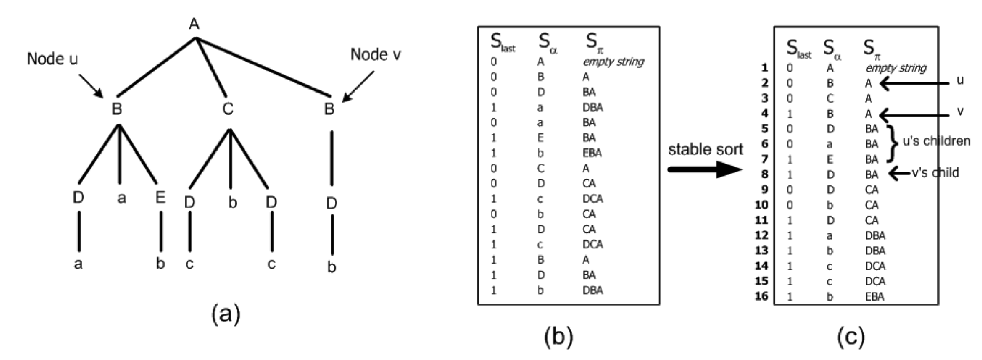
\includegraphics[width=1\textwidth]{Immagini/XBWT_example.png}
    \caption[XBWT example]{(a) A labeled tree $T$ where $\Sigma_N = \{A, B, C, D, E\}$ and $\Sigma_L = \{a, b, c\}$. Notice that $\alpha[u] = \alpha[v] = B$ and $\pi[u] = \pi[v] = A$. (b) The multi-set $S$ is obtained after the pre-order visit of $T$. (c) The final multi-set $S$ after the stable sort based on the $\pi$'s component of its triplets.}
    \label{fig:XBWT_example}
\end{figure}
\end{comment}

\subsubsection{Skew Algorithm}
The Skew algorithm is an efficient method for constructing the suffix array of a string in linear time. A suffix array is a data structure that lists the starting indices of all the suffixes of a string in lexicographical order, and it is widely used in various string processing algorithms.

\subsubsection*{Algorithm Overview}

\subsubsection*{1. Divide the String}

The algorithm begins by partitioning the indices of the string into three groups based on their modulo 3 value:
\begin{itemize}
    \item $S_0$: Indices congruent to 0 mod 3.
    \item $S_1$: Indices congruent to 1 mod 3.
    \item $S_2$: Indices congruent to 2 mod 3.
\end{itemize}

The suffixes starting at positions in $S_1$ and $S_2$ are combined into a single group called $S_{12}$.

\subsubsection*{2. Sort Suffixes in $S_{12}$}

To sort the suffixes in $S_{12}$, the algorithm considers the triplets of characters starting at each position in $S_{12}$. These triplets are sorted using a linear-time sorting algorithm, such as radix sort, and then renamed by assigning each triplet an integer value representing its rank in the sorted order. If all triplets are unique, the sorting is complete; otherwise, the same procedure is applied recursively to the sequence of ranks obtained.

\subsubsection*{3. Sort Suffixes in $S_0$}

Once the suffixes in $S_{12}$ are sorted, the algorithm proceeds to sort the suffixes in $S_0$. To compare two suffixes starting at positions $i$ and $j$ in $S_0$, it compares the first characters of their respective substrings. If the characters are different, their lexicographical order is immediately determined. If they are equal, the algorithm compares the suffixes starting at positions $i+1$ and $j+1$, whose ranks are already known from the sorting of $S_{12}$.

\subsubsection*{4. Merge the Sorted Orders}

Finally, the sorted orders of the suffixes in $S_0$ and $S_{12}$ are merged to obtain the complete suffix array of the original string. This merging process can be performed in linear time, ensuring the overall efficiency of the algorithm.

\subsubsection{PathSort Algorithm} \label{sec:pathSort}

The pseudocode of the pathSort algorithm is shown in \cref{alg:pathSort}. As we can see, the algorithm is based on the Skew algorithm, but it is adapted to work on labeled trees. 
Given a value $j\in\{0,1,2\}$, the main idea is to recursively sort the upward subpaths of the tree starting at nodes in levels $\not\equiv j \pmod{3}$, then sort the upward subpaths starting at nodes in levels $\equiv j \pmod{3}$ using the result of the previous step, and finally merge the two sets of sorted subpaths by exploiting their lexicographic names. $j$ is chosen in such a way that the number of nodes of the shrunk tree whose level is $\equiv j \pmod{3}$ is at least $t/3$ so that a constant fraction of upward paths are ensured to be dropped at each recursive step.
Is important to note that:
\begin{enumerate}
    \item the height of the new (contracted) tree shrinks by a factor of three, hence the node naming requires the radix sort over triples of names; 
    \item given the choice of $j$, the number of nodes of the new (contracted) tree will be at most $2t/3$, thus ensuring that the running time of the algorithm satisfies the recurrence $R(t) = R(2t/3) + \Theta(t) = \Theta(t)$; 
    \item following an argument similar to \cite{karkkainen2006linear}, the names of the dropped subpaths can be computed in $O(t)$ time from the names of the non-dropped subpaths, by radix sorting.
\end{enumerate}

\begin{algorithm}
    \caption{\textsc{PathSort}($T$)}
    \label{alg:pathSort}
    \begin{algorithmic}[1]
    \State Create the array \texttt{IntNodes}[1, $t$], initially empty.
    \State Visit the internal nodes of $T$ in pre-order. Let $u$ denote the $i$-th visited node.
    \State Write in \texttt{IntNodes}[$i$] the symbol $\alpha(u)$, the level of $u$ in $T$, and the position in \texttt{IntNodes} of $u$'s parent.
    \State Let $j \in \{0, 1, 2\}$ be such that the number of nodes in \texttt{IntNodes} whose level is $\equiv j \pmod{3}$ is at least $t/3$. Sort recursively the upward subpaths starting at nodes in levels $\not\equiv j \pmod{3}$.
    \State Sort the upward subpaths starting at nodes in levels $\equiv j \pmod{3}$ using the result of Step 3.
    \State Merge the two sets of sorted subpaths by exploiting their lexicographic names.
    \end{algorithmic}
\end{algorithm}

\subsubsection{Recursive Step of PathSort}
At each recursive step, the algorithm constructs the array \texttt{IntNodes}, which stores the triplets $(\alpha(u), \text{level}(u), \text{parent}(u))$ for every internal node $u$ in the given tree $T$.  

Next, the algorithm selects a value $j$ such that the number of nodes in \texttt{IntNodes} with depth $\equiv j \pmod{3}$ is at least $t/3$. Based on this choice, two separate arrays are created:  
\begin{itemize}
    \item \texttt{IntNodesAtPosJ}, containing nodes at levels $\equiv j \pmod{3}$,
    \item \texttt{IntNodesNotAtPosJ}, containing nodes at levels $\not\equiv j \pmod{3}$
\end{itemize}

For each node $u$ in \texttt{IntNodesNotAtPosJ}, the algorithm extracts the upward path consisting of the first three ancestors of $u$. These paths are then sorted using radix sort. If the sorted upward paths contain duplicates, the algorithm recursively calls the PathSort function on a new contracted tree, where nodes are renamed according to their sorted paths. Otherwise, if all upward paths are unique, the nodes in \texttt{IntNodesAtPosJ} are sorted and subsequently merged with \texttt{IntNodesNotAtPosJ} using lexicographic ordering, following the same merging strategy as in the Skew algorithm.

\subsection{Inversion}
The ability to invert the XBWT is fundamental to its utility as a compression technique. Invertibility guarantees that the original tree can be perfectly reconstructed from its transformed representation ($S_{\text{last}}$ and $S_{\alpha}$). This ensures that the compression is lossless, meaning no information is lost during the process, which is a critical requirement for most applications.

Property 'Path-based Indexing' (\cref{prop3}) ensures that the two arrays $S_{\text{last}}$ and $S_{\alpha}$ of the XBWT can be used to reconstruct the original tree $T$. The algorithm to invert the XBWT is linear in time and requires $O(t \log t)$ bits of space.

\cref{alg:rebuildTree} operates in three main steps. First, it constructs two auxiliary arrays, $F$ and $J$, which are crucial for navigating the tree structure within the compressed format.

\begin{itemize}
    \item \textbf{The $F$ array:} This array maps each character $c \in \Sigma$ to the index of the first occurrence in $S$ of a triplet whose $\pi$-component is prefixed by $c$. It essentially marks the starting points of blocks of nodes that share the same initial path label.
    \item \textbf{The $J$ array:} For each entry $i$ in $S$, $J[i]$ stores the index in $S$ corresponding to the first child of the node represented by $S[i]$. If $S[i]$ represents a leaf, $J[i]$ is set to a sentinel value (e.g., -1).
\end{itemize}

\begin{example}[$F$ and $J$ arrays]
    Considering the XBWT in \cref{tab:xbwt_example}, the $F$ array would map 'A' to index 2 (for node $r$), 'B' to index 5 (for the children of nodes with label 'B'), and so on. For the $J$ array, let's take the node $u$ at index 2 in $S$. Its first child is at index 5. Therefore, $J[2]$ would be 5.
\end{example}

Finally, the algorithm employs the array $J$ to
simulate a depth-first visit of $T$, creates its labeled nodes, and properly connects them to their parents. 

\begin{algorithm}[H]
    \caption{RebuildTree(\texttt{XBWT[$T$]})}
    \label{alg:rebuildTree}
    \begin{algorithmic}[1]
    \State $F = $ BuildF(\texttt{XBWT[$T$]});
    \State $J = $ BuildJ(\texttt{XBWT[$T$]}, $F$); 
    \State Create node $r$ and set $Q = \{\langle1, r\rangle\}$; \Comment{$Q$ is a stack}
    \While{$Q \neq \emptyset$} \Comment{We still have nodes to create in $T$}
        \State $\langle i, u \rangle = $ pop($Q$);
        \State $j = J[i]$; \Comment{Take the block of $u$'s children in $S$}
        \If{$j = -1$} \Comment{$u$ is a leaf of $T$}
            \State \textbf{continue};
        \EndIf
        \State Find first $j' \geq j$ such that $S_{\text{last}}[j'] = 1$; \Comment{$S[j, j']$ are the children of $u$ in $T$}
        \For{$h = j'$ downto $j$} \Comment{Recall that $Q$ is a stack}
            \State Create the node $v$ labeled $S_\alpha[h]$;
            \State Attach $v$ as first child of $u$;
            \State push($\langle h, v \rangle$, $Q$);
        \EndFor
    \EndWhile
    \State \Return node $r$.
    \end{algorithmic}
\end{algorithm}

\begin{algorithm}[H]
    \caption{BuildF(\texttt{XBWT[$T$]})}
    \label{alg:buildF}
    \begin{algorithmic}[1]
    \For{$i = 1, \ldots, |\Sigma_N|$}
        \State $C[S_\alpha[i]] \gets C[S_\alpha[i]] + 1$; \Comment{Count the occurrences of node labels}
    \EndFor
    \State $F[1] = 2$; \Comment{$S_\pi[1]$ is the empty string}
    \For{$i \in \{1, \ldots, |\Sigma_N|-1\}$} \Comment{Consider just the internal-node labels}
        \State $s = 0$; $j = F[i]$;
        \While{$s \neq C[i]$} \Comment{Not all blocks of children have been passed}
            \State $j = j + 1$;
            \If{$S_{\text{last}}[j] = 1$} \Comment{One further block of children has passed}
                \State $s = s + 1$;
            \EndIf
        \EndWhile
        \State $F[i+1] = j$;
    \EndFor
    \State \Return $F$.
    \end{algorithmic}
\end{algorithm}
    
\begin{algorithm}[H]
    \caption{BuildJ(\texttt{XBWT[$T$]}, $F$)}
    \begin{algorithmic}[1]
    \For{$i = 1, \ldots, t$}
        \If{$S_\alpha[i] \in \Sigma_L$}
            \State $J[i] = -1$; \Comment{$S_\alpha[i]$ is a leaf label}
        \Else
            \State $z = J[S_\alpha[i]]$;
            \While{$S_{\text{last}}[z] \neq 1$} \Comment{Reach the last child of $S_\alpha[i]$}
                \State $z = z + 1$;
            \EndWhile
            \State $F[S_\alpha[i]] = z + 1$;
        \EndIf
    \EndFor
    \State \Return $J$.
    \end{algorithmic}
\end{algorithm}

\subsection{Compressing Labeled Trees}
\begin{comment}
Let the $k$-context of a node $u \in T$ be the first $k$ symbols of $\pi(u)$. We denote this $k$-long prefix as $\pi_k[u]$. Thus, $\pi_k[u]$ represents the subpath of length $k$ leading to $u$ in $T$, or equivalently, the node $u$ descends from a subpath labeled as $\pi_k[u]$, where the nodes in $\pi_k[u]$ are encountered in an upward direction.
\end{comment}

The XBWT[$T$] exhibits a local homogeneity property on the string $S_{\alpha}$, specifically, node labels get distributed over $S_{\alpha}$ in accordance with a pattern that clusters closely the labels that descend from `similar' upward paths sharing long prefixes. Which can be demonstrated through the concept of $k$-contexts on trees. 
This property mirrors the strong local homogeneity exhibited by strings under the Burrows-Wheeler Transform \cite{burrows1994block} when applied to labeled trees.

To illustrate this, let us consider two arbitrary nodes $u$ and $v$ in $T$, and examine their contexts $\pi(u)$ and $\pi(v)$. Given the sorting of $S$, the greater the length of the shared prefix between $\pi(u)$ and $\pi(v)$, the closer the corresponding labels $\alpha(u)$ and $\alpha(v)$ will be in the string $S_{\alpha}$. These closely spaced labels are expected to be few in number, resulting in $S_{\alpha}$ exhibiting local homogeneity. As a consequence, we can leverage the advanced algorithmic techniques developed for BWT-based compression methods to achieve efficient compression.

At the end, the XBWT is used for turning the labeled tree compression problem into a string compression problem. To this aim, two string compressors
$C_{\alpha}$ and $C_{\text{last}}$ are used to compress the two strings that compose XBWT[$T$], by exploiting their fine specialties. Of course, many choices are possible for $C_{\alpha}$ and $C_{\text{last}}$, each having implications on the algorithmic time and compression bounds.

In general, the following theorem holds:

\begin{theorem}
    let $C_{\alpha}$ be a $k$-th order string compressor that compresses any string $w$ into $|w|H_k(w) + |w| + o(|w|)$ bits, taking $O(|w|)$ time; and let $C_{\text{last}}$ be an algorithm that stores $S_{\text{last}}$ without compression. With this simple instantiation, the labeled tree $T$ can be compressed within $t H_k(S_{\alpha}) + 2t + o(t)$ bits and takes $O(t)$ optimal time.
\end{theorem}

Since $H_k(S_\alpha) \leq (\log |\Sigma|) + 1,^6$ the above bound is at most $t(\log |\Sigma| + 3) + o(t)$ bits, and can be significantly better than the information-theoretic lower bound and the plain storage of XBWT[$T$] (both taking $2t + t \log|\Sigma|$ bits), depending on the distribution of the labels among its nodes.

\subsection{Indexing a Compressed Labeled Tree} \label{sec:xbwt_operations}
In order to implement the efficient operations listed in \cref{compandindexinglabtree} using the compressed arrays $S_{\text{last}}$ and $S_{\alpha}$ of XBWT, we need that the chosen compressors $C_{\alpha}$ and $C_{\text{last}}$ support the following operations:

Given a string $S[1, t]$ over alphabet $\Sigma$
\begin{itemize}
    \item \textbf{$rank_c(S, q)$}: gives the number of times the symbol $c \in \Sigma$ appears in $S[1, q]$.
    \item \textbf{$select_c(S, i)$}: gives the position of the $i$-th occurrence of the symbol $c \in \Sigma$ in $S$.
\end{itemize}

The compressed indexing of XBWT[$T$] will be based on three compressed data structures that support rank and select queries over the two strings $S_{\alpha}$ and $S_{\text{last}}$, and over an auxiliary binary array $A[1, t]$ defined as: $A[1] = 0$, $A[j] = 1$ if and only if the first symbol of $S_{\pi}[j]$ differs from the first symbol of $S_{\pi}[j - 1]$. 
Hence, $A$ contains at most $|\Sigma| + 1$ bits set to 1 out of $t$ positions. It is also easy to see that, through rank and select operations over $A$, we can succinctly implement the array $F$ employed in \cref{alg:rebuildTree,alg:buildF}.

The following methods are supported by the compressed index:

\textbf{GetRankedChild(i, k)}: Returns the position in $S$ of the $k$-th child of the node at index $i$. If the child does not exist, it returns -1. 
\begin{example}
    In \cref{tab:xbwt_example}, \texttt{GetRankedChild(2, 2)} returns 6.
\end{example}

\textbf{GetCharRankedChild(i, c, k)}: Returns the position in $S$ of the $k$-th child labeled $c$ of the node at index $i$. If the child does not exist, it returns -1.
\begin{example}
    In \cref{tab:xbwt_example}, \texttt{GetCharRankedChild(1, B, 2)} returns 4.
\end{example}

\textbf{GetDegree(i)}: Returns the total number of children of the node at index $i$ in $S$.

\textbf{GetCharDegree(i, c)}: Returns the number of children of the node at index $i$ in $S$ that have the label $c$.

\textbf{GetParent(i)}: Returns the position in $S$ of the parent of the node at index $i$. If the node is the root (at index 1), it returns -1.
\begin{example}
    In \cref{tab:xbwt_example}, \texttt{GetParent(8)} returns 4.
\end{example}

\textbf{GetSubtree(i)}: Retrieves the labels of all nodes in the subtree rooted at the node at index $i$ in $S$. The labels can be returned in any standard traversal order (e.g., pre-order, in-order, or post-order).

\textbf{SubPathSearch($P$)}: For a given labeled path $P = c_1c_2 \cdots c_k$, this function finds the range $S[\text{First} \dots \text{Last}]$ containing the immediate children of all nodes that match the path $P$. Meaning that all strings in $S_{\pi}[\text{First} \dots \text{Last}]$ are prefixed by the reversed path $P^R = c_k \cdots c_2c_1$, as the strings in $S_{\pi}$ are constructed using upward paths.
\begin{example}
    In \cref{tab:xbwt_example}, \texttt{SubPathSearch(BD)} results in the range [12, 13], and \\ \texttt{SubPathSearch(AB)} gives the range [5, 8].
\end{example}

It is important to note that their time complexity is dependent on the specific implementation for rank and select over the compressed strings $S_{\alpha}$ and $S_{\text{last}}$. 

Let's now see how to implement some of the above methods (from which the others can be derived) using the rank and select operations over the compressed strings $S_{\alpha}$ and $S_{\text{last}}$.

\begin{table}
    \centering
    \begin{tabular}{r c c c l}
    \hline\hline
    \textbf{} & $A$ & \textbf{$S_{\text{last}}$} & \textbf{$S_{\alpha}$} & \textbf{$S_{\pi}$} \\
    \hline
    \textbf{1} & 0 & 0 & A & \textit{empty string} \\
    \textbf{2} & 1 & 0 & B & A \\
    \textbf{3} & 0 & 0 & C & A \\
    \textbf{4} & 0 & 1 & B & A \\
    \textbf{5} & 1 & 0 & D & BA \\
    \textbf{6} & 0 & 0 & a & BA \\
    \textbf{7} & 0 & 1 & E & BA \\
    \textbf{8} & 0 & 1 & D & BA \\
    \textbf{9} & 1 & 0 & D & CA \\
    \textbf{10} & 0 & 0 & b & CA \\
    \textbf{11} & 0 & 1 & D & CA \\
    \textbf{12} & 1 & 1 & a & DBA \\
    \textbf{13} & 0 & 1 & b & DBA \\
    \textbf{14} & 0 & 1 & c & DCA \\
    \textbf{15} & 0 & 1 & c & DCA \\
    \textbf{16} & 1 & 1 & b & EBA \\
    \hline\hline
    \end{tabular}
    \caption{The multi-set $S$ for the tree shown in \cref{fig:example_tree}, obtained by stably sorting triplets according to their '$\pi$' components. In this representation, nodes $u$ and $v$ from the original tree $T$ appear at indices $2$ and $4$, respectively. The children's block of node $u$ occupies positions $5$ through $7$, while node $v$'s single child is located at index $8$. Also, the auxiliary binary array $A$ is shown.}
    \label{tab:xbwt_example_2}
\end{table}

\subsubsection*{GetChildren(i)}
\cref{alg:getchildren} exploits directly the properties described before, in particular Property `Path-based Indexing' (\cref{prop3}). The rank operation at line 5 is used to get the number $r$ of nodes labeled $c$ up to position $i$ in $S_{\alpha}$. Then, the position $F[c]$ is obtained through a select operation on $A$ (line 6). By Property `Path-based Indexing', the children of $S[i]$ are located at the $r$-th block of children following position $F[c]$. Lines $8 - 9$ identify this block. 

\begin{example}
    Let's walk through an example using \cref{tab:xbwt_example_2}. Consider the node $u$ at index 2 labeled with $B$. To find its children:

    \begin{enumerate}
        \item First, we compute $r = 1$ since this is the first occurrence of $B$ in $S_{\alpha}$ up to position 2.
        \item Next, we find $y = F[B] = 5$, which marks the start of the block containing children of all nodes labeled $B$.
        \item Then, we count $z = 1$ ones in $S_{\text{last}}$ up to position $y-1$.
        \item Finally, the children block is delimited by the $z+r-1 = 1$st and $z+r = 2$nd ones in $S_{\text{last}}$, giving us the range $[5,7]$.
    \end{enumerate}

    This range $[5,7]$ indeed contains the three children of the node at index 2, as we can verify from the tree structure in \cref{fig:example_tree}.
\end{example}

\begin{algorithm}[H] 
    \caption{GetChildren($i$)}
    \label{alg:getchildren}
    \begin{algorithmic}[1]
    \If{$S_\alpha[i] \in \Sigma_L$}
        \State \Return $-1$ \Comment{$S[i]$ is a leaf}
    \EndIf
    \State $c \gets S_\alpha[i]$ \Comment{$S[i]$ is labeled $c$}
    \State $r \gets \text{rank}_c(S_\alpha, i)$
    \State $y \gets \text{select}_1(A, c)$ \Comment{$y = F[c]$}
    \State $z \gets \text{rank}_1(S_{\text{last}}, y - 1)$
    \State $\text{First} \gets \text{select}_1(S_{\text{last}}, z + r - 1) + 1$
    \State $\text{Last} \gets \text{select}_1(S_{\text{last}}, z + r)$
    \State \Return $(\text{First}, \text{Last})$
    \end{algorithmic}
\end{algorithm}

\subsubsection*{GetParent(i)}
\cref{alg:getparent} is based on Property `Path-based Indexing' (\cref{prop3}) and it is the inverse of the GetChildren method. In line 4, the algorithm computes the label $c$ of the parent of $S[i]$ that prefixes the upward path leading to $S[i]$. Then, the parent of $S[i]$ is searched among the nodes labeled $c$ in $S_{\alpha}$ by exploiting Property `Path-based Indexing' in a reverse manner. Namely, the number $k$ of children-blocks in the range $S[y, i]$ is computed; these are children of nodes labeled $c$ and preceding $i$ in the stable sort of $S$. Then, the $k$-th occurrence of $c$ in $S_{\alpha}$ is selected, which is indeed the parent of $S[i]$.

\begin{example}
    Let's illustrate how to find a node's parent using \cref{tab:xbwt_example_2}. Consider node $v$ located at index 4 with label $B$. The process to find its parent involves:
    \begin{enumerate}
        \item Computing $c = \text{rank}_1(A, 4) = 1$, which tells us the parent has label `A' (as $A$ contains exactly one 1 up to position 4).
        \item Locating $y = F[A] = 2$, which indicates where the block of children for nodes labeled `A' begins.
        \item Calculating $k = \text{rank}_1(S_{\text{last}}, 4-1) - \text{rank}_1(S_{\text{last}}, 2-1) = 0$, meaning no complete child blocks appear before position 4.
        \item Therefore, $v$'s parent is the first ($(k+1)$-th) occurrence of `A' in $S_{\alpha}$, corresponding to index 1 (the root of $\mathcal{T}$).
    \end{enumerate}
    This example demonstrates how the XBWT structure efficiently encodes parent-child relationships using just the $S_{\text{last}}$ and $S_{\alpha}$ arrays.
\end{example}

\begin{algorithm}[H]
    \caption{GetParent($i$)}
    \label{alg:getparent}
    \begin{algorithmic}[1]
    \If{$i = 1$}
        \State \Return $-1$ \Comment{$S[i]$ is the root of $\mathcal{T}$}
    \EndIf
    \State $c \gets \text{rank}_1(A, i)$
    \State $y \gets \text{select}_1(A, c)$
    \State $k \gets \text{rank}_1(S_{\text{last}}, i - 1) - \text{rank}_1(S_{\text{last}}, y - 1)$
    \State $p \gets \text{select}_c(S_\alpha, k + 1)$
    \State \Return $p$
    \end{algorithmic}
\end{algorithm}

\subsubsection*{SubPathSearch($P$)}
We assume that $P = c_1c_2 \cdots c_k$ algorithm SubPathSearch computes the range $[First, Last]$ in $|P| = l$ phases, each one preserving the following invariant:

\begin{itemize}
    \item Invariant of Phase $i$. At the end of the phase, $S_{\pi}[First]$ is the first entry prefixed by $P[1, i]^R$ , and $S_{\pi}[Last]$ is the last entry prefixed by $P[1, i]^R$ , where $s^R$ is the reversal of string $s$.
\end{itemize}

At the beginning (i.e., $i = 1$), First and Last are easily determined via the entries $F[c_1]$ and $F[c_1 + 1] - 1$, which point to the first and last entry of $S_{\pi}$ prefixed by $c_1$ (by definition of array $F$). Since we do not have the $F$ array, we implement these operations via rank and select queries over array $A$. Let us assume that the invariant holds for Phase $i - 1$, and prove that the $i$-th iteration of the for-loop in algorithm SubPathSearch preserves the invariant. More precisely, let $S_{\pi}[First, Last]$ be all entries prefixed by $P[1, i - 1]^R$. So $S[First, Last]$ contains all nodes descending from $P[1, i - 1]$. SubPathSearch determines $S[z_1]$ (respectively $S[z_2]$) as the first (respectively last) node in $S[First, Last]$ that descends from $P[1, i - 1]$ and is labeled $c_i$, if any. Then it jumps to the first child of $S[z_1]$ and the last child of $S[z_2]$. From Property 2 (item 2) and the correctness of algorithms GetChildren and GetDegree, we infer that the positions of these two children are exactly the first (respectively last) entry in $S$ whose $\pi$-component is prefixed by $P[1, i]^R$. 

The time complexity of the SubPathSearch algorithm is $O(l)$, where $l$ is the length of the input path $P$.

\begin{example}
    Consider the tree in \cref{fig:example_tree}, and let $P = BD$. The algorithm \textsc{SubPathSearch}($P$) returns the range $[12, 13]$ through the following steps:

    \begin{enumerate}
        \item Initially, $First = F[B] = 5$ and $Last = F[C] - 1 = 8$. The range $S[5,8]$ contains all nodes descending from paths prefixed by $B$.
        
        \item For $c_2 = D$:
        \begin{itemize}
            \item Compute $k_1 = 0$ and $k_2 = 2$
            \item This yields $z_1 = 5$ and $z_2 = 8$
            \item The first child of $S[5]$ is at position $12$
            \item The last (and only) child of $S[8]$ is at position $13$
        \end{itemize}
        
        \item Therefore, the algorithm returns the range $[12,13]$
    \end{enumerate}

    Note that both the number of offspring and the number of occurrences of subpath $P$ are 2, as evidenced by the two occurrences of 1 in $S_{\text{last}}[12,13]$.
\end{example}

\begin{algorithm}[H]
    \caption{SubPathSearch($P$)}
    \label{alg:subpathsearch}
    \begin{algorithmic}[1]
    \State $First \gets F(c_1)$; $Last \gets F(c_1 + 1) - 1$
    \If{$First > Last$}
        \State \textbf{return} ``$P$ is not a subpath of $T$''
    \EndIf
    \For{$i \gets 2, \dots, k$}
        \State $k_1 \gets \text{rank}_{c_i}(S_\alpha, First - 1)$; $z_1 \gets \text{select}_{c_i}(S_\alpha, k_1 + 1)$
        \Comment{first entry in $S_\alpha[First, t]$ labeled $c_i$}
        \State $k_2 \gets \text{rank}_{c_i}(S_\alpha, Last)$; $z_2 \gets \text{select}_{c_i}(S_\alpha, k_2)$
        \Comment{last entry in $S_\alpha[1, Last]$ labeled $c_i$}
        \If{$z_1 > z_2$}
            \State \textbf{return} ``$P$ is not a subpath of $T$''
        \EndIf
        \State $First \gets \text{GetRankedChild}(z_1, 1)$ \Comment{get the first child of $S[z_1]$}
        \State $Last \gets \text{GetRankedChild}(z_2, \text{GetDegree}(z_2))$ \Comment{get the last child of $S[z_2]$}
    \EndFor
    \State \textbf{return} $(First, Last)$
    \end{algorithmic}
\end{algorithm}

\section{Implementation}
The XBWT data structure has been implemented in C++ using the Succinct Data Structure Library 2.0 (SDSL) for efficient representation and manipulation of compressed data structures. We will develop two algorithms for constructing the XBWT: one efficient linear-time recursive algorithm and one more straightforward iterative algorithm. Also, we will implement the necessary data structures and algorithms for navigating and querying the XBWT, such as parent-child navigation and path-based searches. 

The implementation of the XBWT is based on the descriptions provided in the previous sections. Also, it is available on GitHub at the following link: \url{https://github.com/davide-tonetto-884585/XBWT}.

\subsection{Implementation Choices}
Follows a list of the main choices made during the implementation of the XBWT:
\begin{itemize}
    \item The implementation is not focused on a specific kind of data, such as XML documents or JSON files, but it is designed to work with any kind of labeled tree. 
    \item The construction method takes as input a labeled tree. It constructs directly a compressed indexing scheme based on the Extended Burrows-Wheeler Transform of the tree as described in the previous sections.
    \item For the XBWT to work, we assume that the labels of the leaf nodes of the given labeled tree are lexicographically greater than the labels of the internal nodes. This is necessary to ensure that the navigational and search operations work correctly. \draft{This can be obtained by...} \alessio{spiega come si ottiene questo risultato nel caso le foglie siano più piccole.}
    \item The implementation is based on the Succinct Data Structure Library (SDSL) to handle the compressed data structures generated by the XBWT. The SDSL library provides efficient implementations of various compressed data structures and algorithms, which are essential for representing and querying the XBWT efficiently.
    \item The labels of the alphabet are encoded as integers, starting from 0 to $|\Sigma| - 1$, where $|\Sigma|$ is the cardinality of the alphabet. This encoding respects the order of the labels in the alphabet and allows simplifying and reducing the space needed to store the labels in the compressed data structure. For this reason, the constructor of the XBWT class takes as input a generic labeled tree.
    \item All the operations introduced in \cref{sec:xbwt_operations} are implemented in the XBWT class.
\end{itemize}

\subsection{Succinct Data Structures}
The implementation of the XBWT relies heavily on succinct data structures to achieve space efficiency while maintaining fast query operations. In particular, we use succinct data structures to compress the two main arrays of the XBWT: $S_\alpha$ and $S_{\text{last}}$. These arrays, which can be quite large for substantial trees, benefit significantly from compression.

The compression is achieved through the Succinct Data Structure Library (SDSL), which provides efficient implementations of various compressed data structures. For $S_{\text{last}}$, which is a binary sequence, we utilize a compressed bit vector that supports fast rank and select operations. For $S_\alpha$, which contains labels from a potentially large alphabet, we employ a wavelet tree structure that provides both compression and efficient query capabilities.

The SDSL is a C++ library that provides efficient implementations of various compressed data structures and algorithms. It is used in this project to handle the compressed data structures generated by the XBWT. The SDSL library provides a wide range of succinct data structures, such as bit vectors, wavelet trees, and compressed suffix arrays, which are essential for representing and querying the XBWT efficiently. The library is available at \url{https://github.com/simongog/sdsl-lite} \cite{gbmp2014sea}. Let's see the implementation details of the SDSL data structures used in the XBWT implementation.

\subsubsection{RRR Bit Vector}
The RRR bit vector is designed to provide space-efficient representations of bit vectors while supporting efficient rank and select operations. This data structure implements the RRR (Raman, Raman, and Rao) encoding method, which compresses bit vectors by partitioning them into fixed-size blocks and encoding each block based on its population count (the number of 1s) and specific configuration \cite{raman2002succinct}. 

The space needed for an RRR bit vector of length $n$ with $m$ set bits is $nH_0 + o(n)$ ($\approx \lceil \log \binom{n}{m} \rceil$). 
The rank support is provided by \texttt{sdsl::rank\_support\_rrr}, adding $80$ bits and requiring $O(\log k)$ time for rank queries, where $k$ is the number of set bits. The select support is provided by \texttt{sdsl::select\_support\_rrr}, adding $64$ bits and requiring $O(\log n)$ time for select queries.

This data structure is used to represent the $S_{\text{last}}$, the additional bit in $S_{\alpha}$, and $A$ arrays of the XBWT.

\subsubsection{Wavelet Tree}
The Wavelet tree is designed to efficiently handle sequences over large alphabets, such as integer sequences. It provides a space-efficient representation while supporting fast access, rank, and select operations. The wavelet tree is a balanced binary tree that recursively partitions the alphabet into two equal-sized subsets and encodes the sequence based on the partitioning \cite{grossi2003high}. The \texttt{sdsl::wt\_int} uses the RRR bit vectors or other succinct representations for storing the bit vectors in each node of the wavelet tree. This makes the structure space-efficient.

In the case of RRR bit vectors the space needed by integer Wavelet tree for a sequence of length $n$ over an alphabet of size $\sigma$ is $nH_0(S) + o(n \log \sigma) + \Theta(\sigma \log n)$ bits, where $H_0(S)$ is the zero-order empirical entropy of the sequence $S$. Also supports query access, rank, and select operations in $O(\log \sigma)$ time.

This data structure is used to represent the $S_\alpha$ array of the XBWT.

\begin{comment}
\subsection{Details of the XBWT Class Elements}
\alessio{Questa sezione non mi convince. Non descrivere troppo il codice, la documentazione dovrebbe essere nella repo e nel codice, non nella tesi.}
The XBWT class utilizes several data structures from the SDSL library to efficiently represent and query the compressed data. Below are the details of the main elements used in the class:

\begin{itemize}
    \item \texttt{sdsl::rrr\_vector<> SLastCompressed}: This is a compressed bit vector that stores the $S_{\text{last}}$ array of the XBWT. 
    \item \texttt{sdsl::wt\_int<sdsl::rrr\_vector<>> SAlphaCompressed}: This is a wavelet tree built on top of a compressed bit vector. The wavelet tree is used to compress and index the $S_{\alpha}$ array of the XBWT.
    \item \texttt{sdsl::rrr\_vector<> SAlphaBitCompressed}: Another compressed bit vector used to store the additional bit of $S_{\alpha}$ needed to distinguish between internal and leaf nodes.
    \item \texttt{sdsl::rrr\_vector<> ACompressed}: A compressed bit vector representing the $A$ array of the XBWT used to in the $F$ array of the XBWT.
    \item \texttt{sdsl::rrr\_vector<>::rank\_1\_type SLastCompressedRank}: A rank support structure for the \texttt{SLastCompressed} bit vector, allowing efficient rank queries.
    \item \texttt{sdsl::rrr\_vector<>::select\_1\_type SLastCompressedSelect}: A select support structure for the \texttt{SLastCompressed} bit vector, allowing efficient select queries.
    \item \texttt{sdsl::rrr\_vector<>::rank\_1\_type ACompressedRank}: A rank support structure for the \texttt{ACompressed} bit vector.
    \item \texttt{sdsl::rrr\_vector<>::select\_1\_type ACompressedSelect}: A select support structure for the \texttt{ACompressed} bit vector.
    \item \texttt{std::unordered\_map<T, unsigned int> alphabetMap}: A hash map that maps each label in the alphabet to a unique integer.
    \item \texttt{unsigned int cardSigma}: The cardinality of the alphabet $\Sigma$.
    \item \texttt{unsigned int cardSigmaN}: The cardinality of the $\Sigma_N$ alphabet. Where $\Sigma_N$ is the set of labels that appear in the internal nodes of the labeled tree.
    \item \texttt{unsigned int maxNumDigits}: The maximum number of digits that has the integer code associated to the greater label in the alphabet (needed to sort the labels in the alphabet).
\end{itemize}

The overall space complexity of the XBWT class can be derived from the space complexity of the compressed data structures used in the class. 

\subsection{Construction implementation}
\alessio{Perché non fare pseudocodice come per Alg 1?}
The construction of the XBWT is done by the constructor of the XBWT class. The constructor takes as input a generic labeled tree and constructs the compressed indexing scheme using the linear pathSort (also the naive construction method can be used by passing the boolean flag \texttt{usePathSort = false}). The construction process is divided into the following steps:

\begin{enumerate}
    \item \textbf{Alphabet Encoding}: The first step is to encode the labels of the alphabet as integers. The labels are sorted in lexicographical order and assigned a unique integer code starting from 1 to $|\Sigma|$. Two hash maps are used to map each label to a unique integer and vice versa. 
    \item \textbf{Construct \texttt{intNodes} array}: The next step is to construct the \texttt{intNodes} array as described in the previous chapters. \texttt{intNodes} is an array of triplets of length $t$ in which node is represented as a triplet containing the node's label, its level, and the index of its parent node in the array (from 1 to t, root has parent 0). The nodes are inserted in preorder traversal of the labeled tree.
    \item \textbf{Sort \texttt{intNodes} array:} Call the \texttt{pathSort} or \texttt{upwardStableSortConstruction} (naive method) method to get the sorted array of nodes \texttt{intNodes}.
    \item \textbf{Construct $S_{\text{last}}$ array}: Construct the $S_{\text{last}}$ array by iterating over the sorted \texttt{intNodes} array.
    \item \textbf{Construct $S_{\alpha}$ array}: Construct the $S_{\alpha}$ array by iterating over the sorted \texttt{intNodes} array, along with the additional bit array to distinguish between internal and leaf nodes.
    \item \textbf{Construct $A$ array}: Construct the $A$ array by iterating over the sorted \texttt{intNodes} array.
    \item \textbf{Construct rank and select support structures}: Construct the rank and select support structures for the compressed bit vectors.
\end{enumerate}

\subsection{Navigational Operations}
\alessio{Non basta dire che implementi tutte le funzioni descritte nella sezione 3.7?}

The XBWT class provides several navigational operations to traverse the labeled tree and retrieve information about the nodes. The navigational operations implemented are:

\begin{itemize}
    \item \texttt{getChildren(unsigned int i)}: This method returns a pair of integers representing the indices of the leftmost and rightmost children of the node at index \texttt{i}.
    \item \texttt{getRankedChild(unsigned int i, unsigned int k)}: This method returns the index of the \texttt{k}-th child of the node at index \texttt{i}.
    \item \texttt{getCharRankedChild(unsigned int i, T label, unsigned int k) const}: This method returns the index of the \texttt{k}-th child of the node at index \texttt{i} with the specified label.
    \item \texttt{getDegree(unsigned int i)}: This method returns the degree (number of children) of the node at index \texttt{i}.
    \item \texttt{getCharDegree(unsigned int i, T label)}: This method returns the number of children of the node at index \texttt{i} with the specified label.
    \item \texttt{getParent(unsigned int i)}: This method returns the index of the parent of the node at index \texttt{i}.
    \item \texttt{getSubtree(unsigned int i, unsigned int order = 0)}: This method returns a vector containing the labels of the nodes in the subtree rooted at index \texttt{i}. The \texttt{order} parameter specifies the traversal order (e.g., preorder, post-order).
\end{itemize}

All the methods refer to the index of the nodes in $S_{\text{last}}$ and $S_{\alpha}$ arrays. 

\subsection{Search Operations}
The XBWT class provides search operation \texttt{subPathSearch(const std::vector<T> \&path)} that searches for a subpath in the XBWT structure. It uses the compressed vectors to determine the range of positions corresponding to the nodes whose upward path is prefixed by a given vector reversed.

\end{comment}

\subsection{Construction Time Experiments} 

To evaluate the performance of the implemented algorithms, we conducted a series of experiments on randomly generated trees, with sizes ranging from 100 to 900,000 nodes. For each tree, we executed the construction algorithms 10 times, recording the average execution time for both the linear \textsc{PathSort} algorithm and the Naive Sort algorithm used for constructing the XBWT.
By ``Naive Sort'', we refer to a straightforward approach that first precomputes all the upward paths in the tree and then sorts them using a standard sorting algorithm. This method contrasts with \textsc{PathSort}, which is specifically designed to achieve linear time complexity in path sorting.
This approach enabled us to compare their performance across various tree sizes and evaluate their scalability.

From the results shown in Table \cref{tab:experiments}, we can draw several conclusions about the performance of the \textsc{PathSort} algorithm compared to the Naive Sort algorithm.

The \textsc{PathSort} algorithm consistently outperforms the Naive Sort algorithm in terms of execution time, especially as the number of nodes increases. For smaller trees, the difference in execution time between the two algorithms is minimal. However, as the number of nodes grows, the \textsc{PathSort} algorithm demonstrates significantly better scalability. For instance, with 900,000 nodes, the \textsc{PathSort} algorithm takes 8.51 seconds, whereas the Naive Sort algorithm takes 34.2 seconds, giving a speedup of more than $4\times$. A visual representation of the results can be seen in \cref{fig:xbwt_exp_plots} where both the time comparison and the speedup are shown.

\begin{table}[h]
    \centering
    \begin{tabular}{|r|r||r|r|}
        \hline
        \textbf{\# Nodes} & \textbf{Depth} & \textbf{Naive Sort (s)} & \textbf{\textsc{PathSort} (s)} \\
        \hline
            100 &    22 &  0.001 & 0.002 \\
            500 &    45 &  0.002 & 0.004 \\
          1,000 &    74 &  0.003 & 0.006 \\
          5,000 &   175 &  0.015 & 0.028 \\
         10,000 &   288 &  0.053 & 0.056 \\
         50,000 &   486 &  0.350 & 0.310 \\
        100,000 &   754 &  1.250 & 0.690 \\
        500,000 & 2,246 & 16.460 & 4.700 \\
        900,000 & 2,658 & 34.200 & 8.510 \\
        \hline
    \end{tabular}
    \caption{Performance comparison of the execution times for the Naive Sort and \textsc{PathSort} algorithms on randomly generated trees of varying sizes.}
    \label{tab:experiments}
\end{table}

\begin{figure}[H]
    \centering
    \begin{subfigure}[b]{0.48\textwidth}
        \centering
        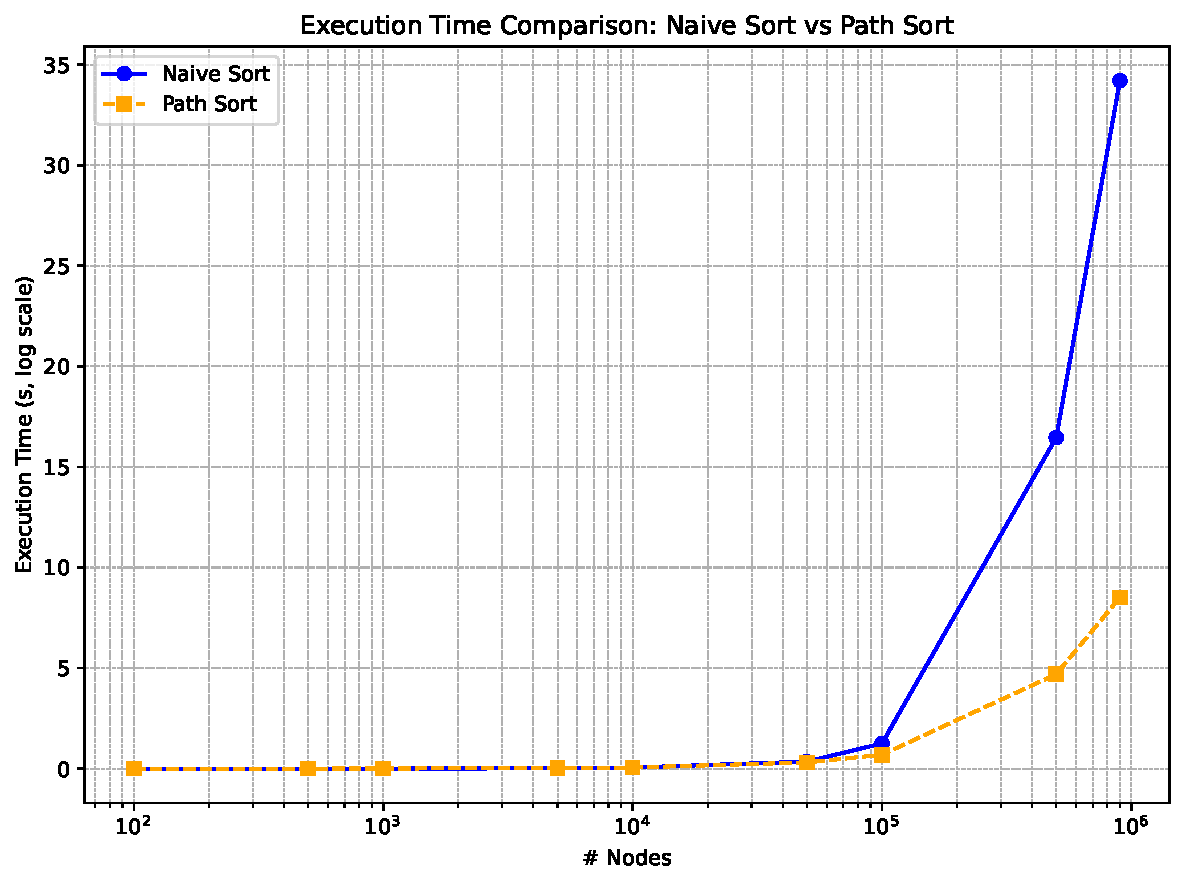
\includegraphics[width=\textwidth]{"Immagini/execution_time_comparison.pdf"}
        \caption{Time Comparison}
        \label{fig:time_comparison}
    \end{subfigure}
    \hfill %
    \begin{subfigure}[b]{0.48\textwidth}
        \centering
        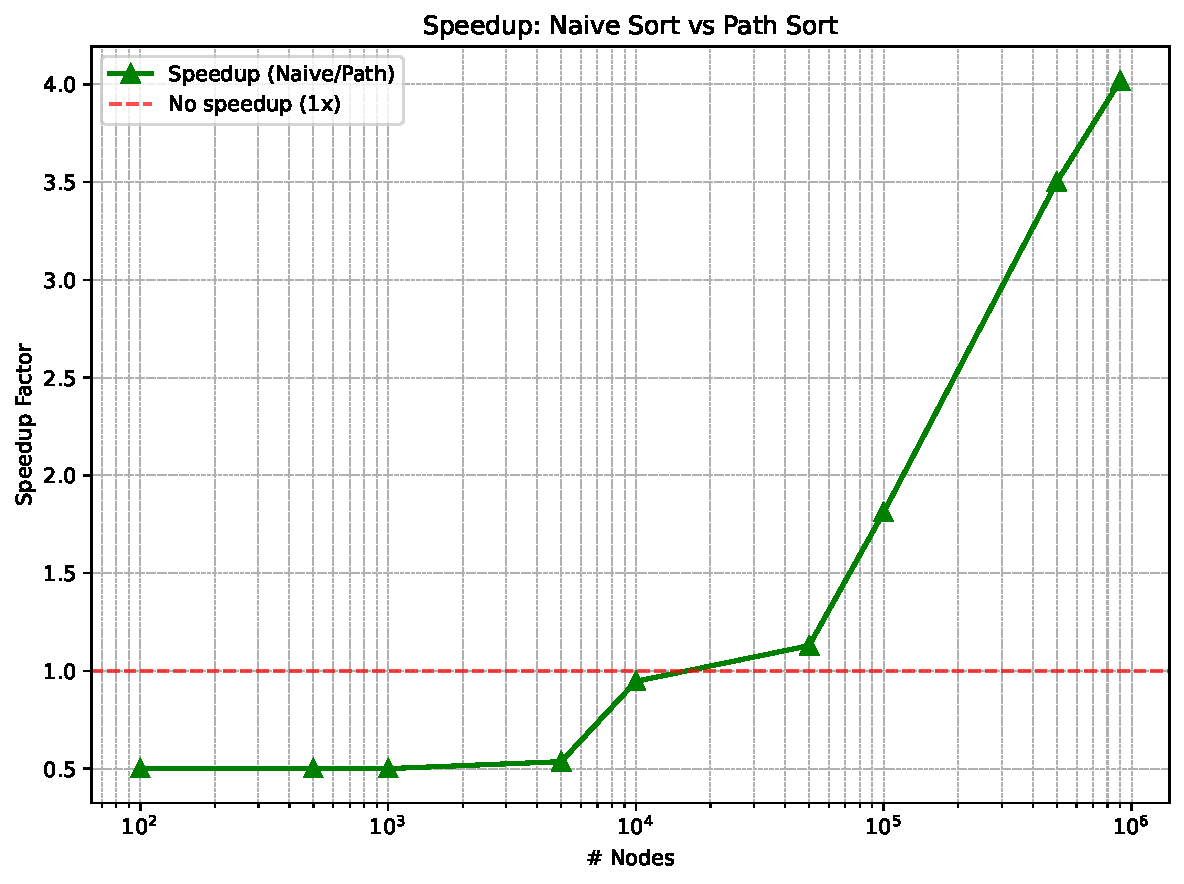
\includegraphics[width=\textwidth]{"Immagini/speedup_comparison.pdf"}
        \caption{Speedup}
        \label{fig:speedup}
    \end{subfigure}
    \caption{Time comparison and speedup plots for the experiments in \cref{tab:experiments}. Image (a) shows \textsc{PathSort} time in seconds (yellow dashed line) vs. Naive Sort time (blue line). Image (b) shows the speedup of \textsc{PathSort} over Naive Sort. The area below the red dashed line indicates points where the speedup is less than or equal to 1, representing no improvement of \textsc{PathSort} over Naive Sort.}
    \label{fig:xbwt_exp_plots}
\end{figure}

\begin{comment}
\subsubsection{Space Analysis}
To evaluate the space savings achieved through XBWT compression, we conducted experiments on the same set of randomly generated trees used for the construction performance tests. For each tree, we compared the memory usage (in bytes) of three representations: the plain tree, the uncompressed XBWT, and the compressed XBWT.

The plain tree representation consists of the simple balanced parentheses encoding of the tree structure combined with the edge labels. For example, for the tree in \cref{fig:example_tree,tab:xbwt_example}, the plain tree representation would be:

\texttt{(A(B(D(a))(a)(E(b)))(C(D(c))(b)(D(c)))(B(D(b))))}.

By \emph{uncompressed XBWT}, we refer to the XBWT arrays $S_{\text{last}}$ and $S_{\alpha}$ (including the additional bit) stored without any compression. Specifically, $S_{\text{last}}$ is represented as a plain bitvector (\texttt{sdsl::bit\_vector}), and $S_{\alpha}$ is stored as a wavelet tree (\texttt{sdsl::wt\_int}) with plain bitvectors (\texttt{sdsl::bit\_vector}). In contrast, the \emph{compressed XBWT} representation stores $S_{\text{last}}$ and $S_{A}$ as compressed RRR bitvectors (\texttt{sdsl::rrr\_vector}), and $S_{\alpha}$ as a wavelet tree with RRR bitvectors, as described in the previous chapter.

\cref{tab:experiments_2} reports the sizes (in bytes) for each representation of the trees across different sizes. The last column highlights the space savings achieved by the compressed XBWT compared to the plain tree representation, expressed as a percentage. These results illustrate the substantial space reductions achieved through compression, especially as the tree size increases.

%\alessio{Oltre ai punti di prima, metti la percentuale anche per UXBWT, magari non come un'altra colonna ma metti tra parentesi. Te lo faccio sulle prime righe per la C.XBWT. Se ti piace, ricorda di spiegare cosa sono i numeri tra parentesi nella descrizione.}
\begin{table}[ht]
    \centering
    \begin{tabular}{|r||r|r|r|}
        \hline
        \textbf{\# Nodes} & \textbf{Plain tree} & \textbf{U. XBWT} & \textbf{C. XBWT} \\
        \hline
            100 &       390 &       424 &       496 \color{gray}{(-27.18\%)}\\
            500 &     2,390 &     1,112 &     1,136 ~\color{gray}{(52.47\%)} \\
          1,000 &     4,890 &     2,242 &     2,056 ~\color{gray}{(57.96\%)} \\
          5,000 &    28,890 &    12,911 &    10,400 ~\color{gray}{(64.00\%)} \\
         10,000 &    58,890 &    45,625 &    21,848 ~\color{gray}{(62.90\%)} \\
         50,000 &   338,890 &   175,146 &   123,216 ~\color{gray}{(63.64\%)} \\
        100,000 &   688,890 &   349,478 &   259,376 ~\color{gray}{(62.35\%)} \\
        500,000 & 3,888,890 & 1,850,850 & 1,451,570 ~\color{gray}{(62.67\%)} \\
        900,000 & 7,088,890 & 3,480,190 & 2,718,570 ~\color{gray}{(61.65\%)} \\
        \hline
    \end{tabular}
    \caption{Space analysis of the XBWT. The first column represents the number of nodes, the others the bytes used by each representation.
    ``Plain tree'' is the size of the tree in the simple balanced parenthesis representation plus the edge labels, ``U. XBWT'' is the size of the uncompressed XBWT, and ``C. XBWT'' is the size of the compressed XBWT.
    Gray numbers between parentheses represent the improvement relative to the plain tree representation.}
    \label{tab:experiments_2}
\end{table}

For small trees, the compressed XBWT does not always provide immediate savings due to the overhead of succinct data structures. For instance, for 100 nodes, the compressed representation is larger than the plain tree, showing a \(-27.18\%\) increase in space. However, as the number of nodes increases, the compression becomes more effective, achieving savings of over 60\% for large trees.

The space reduction becomes particularly evident for trees with more than 500 nodes. These results confirm that the compressed XBWT provides a scalable and space-efficient alternative for storing and indexing labeled trees. The efficiency gains are particularly beneficial for applications requiring large-scale tree processing, such as bioinformatics and text indexing.
\end{comment}

\newpage
\
\newpage
\chapter{DFA Minimization} \label{chp:hopcroft}

\section{Introduction and Motivation}
Tree compression schemes that effectively exploit repetitive structures require efficient techniques for identifying and representing such repetitions compactly. A powerful approach to this problem is to view a tree as a finite language, where each path from the root to a leaf represents a word. Such a language can be recognized by a Deterministic Finite Automaton (DFA). More specifically, since trees are inherently acyclic, they can be represented by Acyclic Deterministic Finite Automata (ADFAs).

The problem of finding and compressing identical subtrees is thus equivalent to minimizing the corresponding DFA. DFA minimization ensures that equivalent substructures are merged efficiently, leading to a more compact encoding. The minimized DFA provides a canonical representation of the repetitive structures, which can then be leveraged in our compression pipeline. This theoretical foundation enables us to identify and encode tree patterns systematically, ultimately improving the compression efficiency.

While general-purpose minimization algorithms like Hopcroft's are highly efficient for any DFA, the specific structure of ADFAs allows for even faster, linear-time algorithms. In this context, we focus on Revuz's algorithm, which is specifically designed to minimize ADFAs and is therefore particularly well-suited for compressing tree structures.

This chapter provides the necessary theoretical background on DFA minimization. We will first introduce the concepts of DFAs and their minimization, followed by a detailed look at both Hopcroft's algorithm as a general solution and Revuz's algorithm as a specialized, linear-time solution for acyclic graphs, which is central to our tree compression methodology.

\section{Deterministic Finite Automata}
\begin{definition}[Deterministic Finite Automaton] \label{def:dfa}
    A deterministic finite automaton (DFA) is a 5-tuple $M = (Q, \Sigma, \delta, q_0, F)$ where:
    \begin{itemize}[leftmargin=25pt]
        \item $Q$ is a finite set of states
        \item $\Sigma$ is a finite set of input symbols (alphabet)
        \item $\delta: Q \times \Sigma \rightarrow Q$ is the transition function
        \item $q_0 \in Q$ is the initial state
        \item $F \subseteq Q$ is the set of final (accepting) states
    \end{itemize}
\end{definition}

The DFA processes an input string $s$ one symbol at a time by starting from the initial state $q_0$ and following transitions based on the input symbols. The string $s$ is accepted if the DFA ends in an accepting state after processing all input symbols; otherwise, it is rejected. The language recognized by a DFA is the set of all strings that lead to an accepting state. DFAs are widely used in various applications, including lexical analysis, pattern matching, and formal language theory. 

\subsection{DFA Minimization}
The process of automata minimization consists of reducing the number of states in a DFA while preserving the language accepted by the DFA. The minimization of DFA is crucial for a variety of applications, such as model checking, hardware design, and compilers, as it produces a more effective and compact representation of the automaton, allowing for faster processing and reduced memory usage.

The minimization of DFA is a well-studied problem in automata theory, and there are several algorithms available for this purpose. One of the most popular algorithms for DFA minimization is Hopcroft's algorithm, which was proposed by John Hopcroft in 1971 \cite{HOPCROFT1971189}. Hopcroft's algorithm is an efficient and simple algorithm that can minimize a DFA in $O(n \log n)$ time, where $n$ is the number of states in the DFA.

\section{Hopcroft's Minimization Algorithm}
DFA minimization is a classical and widely studied problem in Automata Theory and Formal Languages. It consists of finding the unique (up to isomorphism) finite automaton with the minimal number of states, recognizing the same regular language of a given DFA.

\begin{algorithm}
    \caption{Hopcroft's Algorithm for DFA Minimization} \label{alg:DFA_min}
    \begin{algorithmic}[1]
    \Require $M = (Q, \Sigma, \delta, q_0, F)$
    \Function{HopcroftMinimization}{$M$}
    
    \State $P \gets \{F, Q \setminus F\}$ \Comment{Initial partition}
    \State $W \gets \{F\}$ \Comment{Working set initialized with final states}
    
    \While{$W \neq \emptyset$}
        \State Remove a set $A$ from $W$
        \ForAll{$c \in \Sigma$}
            \State $X \gets \{q \in Q \mid \delta(q, c) \in A\}$ \Comment{Predecessors of $A$ via $c$}
            \ForAll{$Y \in P$ such that $X \cap Y \neq \emptyset$ and $Y \setminus X \neq \emptyset$}
                \State Replace $Y$ in $P$ with $Y_1 = X \cap Y$ and $Y_2 = Y \setminus X$
                \If{$Y \in W$}
                    \State Replace $Y$ in $W$ with $Y_1$ and $Y_2$
                \Else
                    \State Add the smaller of $Y_1$ and $Y_2$ to $W$
                \EndIf
            \EndFor
        \EndFor
    \EndWhile
    
    \State \Return the minimized DFA built from partition $P$
    \EndFunction
    \end{algorithmic}
\end{algorithm}

Algorithm \cref{alg:DFA_min} works by iteratively refining a partition of the states until no further refinement is possible, meaning all states within each set of the partition are indistinguishable. The final partition represents the equivalence classes, which correspond to the states of the minimal DFA. Here's a step-by-step explanation based on the provided pseudocode:

\begin{enumerate}
    \item \textbf{Initialization:} The algorithm starts with an initial partition $P$ containing two sets: the set of final states $F$ and the set of non-final states $Q \setminus F$. These are the coarsest sets of potentially distinguishable states. A working set $W$ is initialized, typically containing the set of final states $F$ (or the smaller of the two initial sets as an optimization). $W$ holds the sets that are used as ``splitters'' to refine the partition $P$. These sets are called ``splitters'' because they are used to partition other sets into smaller, more refined ones. A set $A \in W$ acts as a criterion to distinguish states: if for a given symbol, some states in a set $Y$ transition to a state in $A$ and others do not, then $Y$ is split.

    \item \textbf{Refinement Loop:} The algorithm iterates as long as the working set $W$ is not empty. In each iteration, a set $A$ (a ``splitter'') is removed from $W$. Then, for each input symbol $c \in \Sigma$:
        \begin{itemize}
            \item Calculate the set $X = \{q \in Q \mid \delta(q, c) \in A\}$. This is the set of all states that transition into the set $A$ upon reading symbol $c$.
            \item For each set $Y$ currently in the partition $P$, check if $Y$ needs to be split by $X$. A split is necessary if some states in $Y$ are in $X$ and some are not (i.e., $X \cap Y \neq \emptyset$ and $Y \setminus X \neq \emptyset$). This indicates that states in $Y$ are distinguishable based on whether their $c$-transition leads into $A$.
            \item If $Y$ needs to be split, replace $Y$ in the partition $P$ with two new sets: $Y_1 = X \cap Y$ (states in $Y$ that transition into $A$) and $Y_2 = Y \setminus X$ (states in $Y$ that do not transition into $A$).
            \item Update the working set $W$: If the original set $Y$ was in $W$, remove $Y$ and add both new sets $Y_1$ and $Y_2$ to $W$. If $Y$ was not in $W$, add only the smaller of the two new sets ($Y_1$ or $Y_2$) to $W$. This optimization helps maintain the algorithm's efficiency.
        \end{itemize}

    \item \textbf{Termination:} The loop continues until the working set $W$ is empty. At this point, no set in the partition $P$ can be further refined. The partition $P$ now contains the final equivalence classes of states.

    \item \textbf{Result:} The final partition $P$ defines the states of the minimized DFA. Each set in $P$ corresponds to a single state in the minimal DFA, and transitions are defined based on the original DFA's transitions between these sets.
\end{enumerate}

The algorithm enables computing equivalence classes of nodes in $O(n\log n)$, in particular, the Myhill-Nerode equivalence classes \cite{nerode1958linear, myhill1957finite}. The Myhill-Nerode theorem states that a language is regular if and only if it has a finite number of Myhill-Nerode equivalence classes. This theorem provides a powerful tool for determining the regularity of languages and is a cornerstone of automata theory. Let's formalize the concept of equivalence classes and the Myhill-Nerode theorem.

\begin{definition}[Equivalence Relation]
    For a language $L \subseteq \Sigma^*$ and any strings $x,y \in \Sigma^*$, we say $x$ is equivalent to $y$ with respect to $L$ (written as $x \approx_L y$) if and only if for all strings $z \in \Sigma^*$:
    \[ xz \in L \Leftrightarrow yz \in L \]
\end{definition}
That is, strings $x$ and $y$ are equivalent if they have the same behavior with respect to the language $L$: either they both lead to acceptance or both lead to rejection when any suffix $z$ is appended.

\begin{definition}[Regular Language]
    A language $L$ over an alphabet $\Sigma$ is called a \textbf{regular language} if it can be recognized by a deterministic finite automaton (DFA).
\end{definition}

\begin{theorem}[Myhill-Nerode theorem \cite{nerode1958linear,myhill1957finite}] \label{def:myhill-nerode}
    Let $L$ be a language over an alphabet $\Sigma$. Then $L$ is regular if and only if there exists a finite number of Myhill-Nerode equivalence classes for $L$. Specifically, the number of equivalence classes is equal to the number of states in the minimal DFA recognizing $L$.
\end{theorem}

\section{Minimization of Acyclic DFA in Linear Time} \label{sec:revuz}
For our purpose, we will focus on a specific type of finite automaton: an acyclic deterministic finite automaton. An ADFA is a DFA where the transition graph contains no cycles. This structure is also commonly known as a Directed Acyclic Word Graph (DAWG) when used to represent a set of strings. The acyclic property is key, as it simplifies the minimization process significantly. 

In this section, we will discuss an efficient algorithm for minimizing acyclic deterministic finite automata in linear time on the number of states \cite{revuz1992minimisation}. Notice that we will use the following notation for DAWG: for a state $q$ and a symbol $a$, the transition $\delta(q,a)$ will be denoted as $q.a$. This notation is extended to words, so for a word $w = w_1w_2\dots w_n$, $q.w$ is the state reached from $q$ by following the path labeled by $w$. A word $w$ is accepted by the automaton if $q_0.w \in F$.

Let's start by giving some definitions and theorems introduced in the paper \cite{revuz1992minimisation}.

\begin{definition}[Height function] \label{def:height}
    For a state $s$ in an automaton, the height $h(s)$ is defined as the length of the longest path starting at $s$ and going to a final state. 

    $$h(s) = \max\{|w|:s.w \text{ is final}\}$$
\end{definition}

This height function induces a partition $\Pi_i$ of $Q$, where $\Pi_i$ denotes the set of states of height $i$.

\begin{definition}[Distinguished set]
    We say that a set $\Pi_i$ is distinguished if no pair of states in $\Pi_i$ are equivalent.
\end{definition}

\subsection{Algorithm}
The minimization algorithm introduced in \cite{revuz1992minimisation} operates by labeling each state with a unique identifier that represents the structure of the automaton from that state onward. It proceeds in the following steps:

\begin{enumerate}
    \item \textbf{Height Computation:} The height of each state is determined (\cref{def:height}).
    \item \textbf{State Labeling:} Each state is labeled based on the structure of its transitions. The label consists of:
    \begin{itemize}
        \item Whether the state is final or not.
        \item The transitions, recorded as ordered pairs of symbols and target state identifiers.
    \end{itemize}
    Therefore, the resulting structure of each state $s$ is the following:
    $$label(s) = (F/NF, l_1, nl_1, l_2, nl_2, \dots, l_k, nl_k)$$
    where $F/NF$ indicates final/non-final, $l_k$ is the $k$-th transition symbol, and $nl_k$ is the (renumbered) target state name.

    \begin{example}
        Consider a state $s$ at height $i=2$ that is non-final and has two transitions: one on symbol `a' to a state $t_1$ (which belongs to an equivalence class that has been renumbered to 5) and another on symbol `b' to a state $t_2$ (belonging to an equivalence class renumbered to 8). The label for state $s$ would be $(NF, a, 5, b, 8)$.
    \end{example}
    \item \textbf{Lexicographic Sorting:} States at each height level are sorted lexicographically based on their labels using a bucket sort technique.
    \item \textbf{Merging Equivalent States:} After sorting, states with identical labels are merged, ensuring that equivalent states are unified.
\end{enumerate}

In detail, the algorithm minimizes a DAWG by leveraging the concept of state height. The algorithm partitions the states based on their height. It then processes these groups in increasing order of height, starting from height 0.
% \alessio{Dettaglio che ho scoperto anche io un mese fa: la partizione è l'insiseme dei sottoinsiemi, i sottoinsiemi che formano la partizione si chiamano ``groups''.}

The core idea relies on the `height property': If every $\Pi_j$ with $j < i$ is distinguished, then two states $p$ and $q$ in $\Pi_i$ (the set of states with height $i$) are equivalent if and only if for every letter $a$ in the alphabet $\Sigma$, the transitions $p.a$ and $q.a$ lead to the same state (or both are undefined).

The algorithm iteratively ensures that each $\Pi_i$ is distinguished. It starts with $\Pi_0$, where all states are trivially equivalent (as they are final states with no outgoing paths to other final states contributing to height) and merges them. Then, for each subsequent height $i$, it sorts the states in $\Pi_i$ based on their transitions. Specifically, states are grouped based on the target states of their transitions for each symbol in the alphabet. Since all lower levels ($j < i$) are already distinguished by the inductive step, states in $\Pi_i$ that have identical transitions for all symbols (leading to equivalent states in lower levels) are themselves equivalent according to the height property. These equivalent states are then merged.

This process uses a specialized lexicographic sorting technique (related to bucket sort) optimized for this task, which helps achieve linear time complexity relative to the size of the automaton (number of states and transitions). The algorithm leverages a technique similar to the one presented in \cite{aho1974design} for testing tree isomorphism. Specifically, Revuz adopts a renumbering scheme during the lexicographic sorting phase to optimize both time and space complexity. 

\subsubsection{Renumbering Scheme}
The core minimization algorithm relies on sorting states at the same height level based on their transitions. The challenge arises when performing the lexicographic sort (using repeated bucket sorts) on these labels, specifically concerning the $nl_i$ components. If the actual state numbers (ranging from $1$ to $|Q|$, the total number of states) are used directly as the values for $nl_i$:
\begin{itemize}
    \item The range of values for these components becomes large ($1$ to $|Q|$). This forces the bucket sort step that handles these components to use a bucket array of size $|Q|$, potentially making the sort non-linear in the size of the automaton if $|Q|$ is large compared to the number of transitions $e$.
    \item Alternatively, representing state numbers as strings of digits would increase the length of the labels by a factor proportional to $\log |Q|$, again potentially breaking the overall linear time complexity.
\end{itemize}

The renumbering scheme overcomes this issue by assigning temporary, small integer names to the target states ($nl_i$) during the sorting process for each height level $\Pi_i$. The key idea is that when sorting states at height $i$, we only need to distinguish between the equivalence classes of the target states $nl_j$ from lower levels ($j < i$), as those levels have already been processed and minimized. The renumbering scheme ensures that the bucket array size is bounded by the maximum between $|\Sigma|$ (the alphabet size) and $|E_i|$ (the total number of edges from states at height i). The renumbering function adopted is presented in \cref{alg:renumbering}.

\begin{algorithm}[H]
    \caption{Renumbering Function}
    \label{alg:renumbering}
    \begin{algorithmic}[1]
        \Function{Renumber}{s, h, n}
            \If{$s.\text{ch} \ne h$}
                \State $s.\text{ch} = h$
                \State $s.\text{num} = n$
                \State $n = n + 1$
            \EndIf
            \State \Return $s.\text{num}$
        \EndFunction
    \end{algorithmic}
\end{algorithm}

\subsection{Pseudocode}
The paper presents \cite{revuz1992minimisation} the core minimization logic and a more detailed sorting (or distinguishing) algorithm separately. \cref{alg:minimization-dawg} shows a combined representation based on the `Final algorithm' section of the paper.

\begin{algorithm}[H]
    \caption{Minimization Algorithm for DAWGs}
    \label{alg:minimization-dawg}
    \begin{algorithmic}[1]
    \State Calculate height $h(s)$ for every state $s$.
    \State Create partitions $\Pi_i = \{s \in Q \mid h(s) = i\}$.
    \State Merge all states in $\Pi_0$.
    \For{$i := 1$ to $h(q_0)$} \Comment{$q_0$ is the initial state}
        \State \Comment{Distinguish states in $\Pi_i$ using the sorting/distinguishing algorithm below}
        \State Put states in $\Pi_i$ into a list $L$. \Comment{May pre-split by Final/NonFinal}
        \State Call Distinguish($L$)
        \State Merge resulting groups of equivalent states identified by Distinguish.
    \EndFor
    \end{algorithmic}
\end{algorithm}

\cref{alg:distinguish} distinguishes states within a given height level $\Pi_i$. It iteratively refines partitions based on transitions. The sorting happens component by component.

\begin{algorithm}[h]
    \caption{Distinguish Algorithm} \label{alg:distinguish}
    \begin{algorithmic}[1] 
        \Function{Distinguish}{List\_of\_States}
        \State Place List\_of\_States into QUEUE2 \Comment{Queue of lists of potentially equivalent states}
        \State $k := 0$ \Comment{Represents the component index of the label being compared}
        \Repeat
            \State Move QUEUE2 to QUEUE1; Clear QUEUE2
            \State $k := k + 1$
            \While{QUEUE1 not empty}
                \State Let $L$ be the first list in QUEUE1
                \State Clear Buckets $Q[1 \dots m]$ \Comment{$m$ depends on alphabet size and renumbered state names}
                \State Clear NONEMPTY list of bucket indices
                \While{$L$ not empty}
                    \State Let $S$ be the first state in $L$
                    \State Determine the $k$-th component value $v$ for state $S$
                    \If{$Q[v]$ is empty}
                        \State Add $v$ to NONEMPTY
                    \EndIf
                    \State Move $S$ from $L$ to bucket $Q[v]$
                \EndWhile
                \For{each index $v$ in NONEMPTY}
                    \If{Bucket $Q[v]$ contains more than one state}
                        \State Add $Q[v]$ as a list to QUEUE2 \Comment{These still need further distinguishing}
                    \ElsIf{$k$ corresponds to the end-of-label marker '$S$'}
                        \State Merge all states in $Q[v]$ (they are equivalent)
                    \EndIf
                \EndFor
            \EndWhile
        \Until{QUEUE2 is empty} \Comment{No more lists need refinement}
        \EndFunction
    \end{algorithmic}
\end{algorithm}

\textit{Note:} The pseudocode in the paper is slightly intertwined with the bucket sort details. This representation attempts to capture the logic described. The renumbering function is called implicitly when accessing $nl_j$. The handling of merging might occur after the Distinguish procedure completes for level $i$, or potentially within it as groups become fully distinguished. The pseudocode merges states within bucket Q[\$], which relates to the end-of-string marker in the generic sort; for state labels, equivalence is confirmed when a group remains together after checking all label components.

\begin{example} 
    \label{ex:DAWG_minimization}
    Now we are going to see an example of reduction for a given DAWG. The DAWG is represented in figure \cref{fig:example_dawg} and, as we can notice, it is also a valid ordered rooted tree with $n = 11$ nodes, $e = 10$ edges, and the following alphabet: $\Sigma = \{0, 1\}$. The node $a$ is the root of the tree and the initial state of the automaton, while the leaf nodes $e,g,h,i,l,m$ are final states. It is important to note that while the algorithm applies to any DAWG, our focus is on those that are also trees, as this is the specific case relevant to our work.

    \begin{figure}[H]
        \centering
        \begin{tikzpicture}[
            level distance=1.5cm,
            sibling distance=3cm,
            state/.style={circle, draw, minimum size=7mm},
            accepting/.style={circle, draw, double, minimum size=7mm},
            edge from parent/.style={draw, -latex},
            level 1/.style={sibling distance=4cm},
            level 2/.style={sibling distance=2.5cm},
            level 3/.style={sibling distance=2cm}
            ]
        
        \node[state] (a) {a}
            child {node[state] (b) {b} 
            child {node[state] (d) {d}
                child {node[accepting] (h) {h}}
                child {node[accepting] (i) {i}}
            }
            child {node[accepting] (e) {e}}
            }
            child {node[state] (c) {c}
            child {node[state] (f) {f}
                child {node[accepting] (l) {l}}
                child {node[accepting] (m) {m}}
            }
            child {node[accepting] (g) {g}}
            };
        
        % Etichette degli archi
        \path (a) -- (b) node[midway, left] {0};
        \path (a) -- (c) node[midway, right] {1};
        \path (b) -- (d) node[midway, left] {0};
        \path (b) -- (e) node[midway, right] {1};
        \path (c) -- (f) node[midway, left] {0};
        \path (c) -- (g) node[midway, right] {1};
        \path (d) -- (h) node[midway, left] {0};
        \path (d) -- (i) node[midway, right] {1};
        \path (f) -- (l) node[midway, left] {0};
        \path (f) -- (m) node[midway, right] {1};
        \end{tikzpicture}
        \caption{Example DAWG to be minimized}
        \label{fig:example_dawg}
    \end{figure}

    Now, let's apply the minimization algorithm step by step:
    \begin{enumerate}
        \item \textbf{Height Computation:} First, we compute the height of each state. The height is the length of the longest path to a final state. The final states ($e, g, h, i, l, m$) have a height of 0. For the other states, the height is calculated as follows:
        \begin{itemize}
            \item $h(d) = 1 + \max(h(h), h(i)) = 1 + 0 = 1$
            \item $h(f) = 1 + \max(h(l), h(m)) = 1 + 0 = 1$
            \item $h(b) = 1 + \max(h(d), h(e)) = 1 + \max(1, 0) = 2$
            \item $h(c) = 1 + \max(h(f), h(g)) = 1 + \max(1, 0) = 2$
            \item $h(a) = 1 + \max(h(b), h(c)) = 1 + \max(2, 2) = 3$
        \end{itemize}
        This gives us the following partitions based on height:
        \begin{itemize}
            \item $\Pi_0 = \{e, g, h, i, l, m\}$
            \item $\Pi_1 = \{d, f\}$
            \item $\Pi_2 = \{b, c\}$
            \item $\Pi_3 = \{a\}$
        \end{itemize}

        \item \textbf{Processing $\Pi_0$:} All states in $\Pi_0$ are final and have no outgoing transitions, so they are all equivalent. We merge them into a single class, let's call it $D = \{e, g, h, i, l, m\}$. After this step, we have a new state $D$ which is final.

        \item \textbf{Processing $\Pi_1$:} Now we examine the states in $\Pi_1$: $d$ and $f$. We check their transitions:
        \begin{itemize}
            \item State $d$: $\delta(d, 0) = h \in D$ and $\delta(d, 1) = i \in D$.
            \item State $f$: $\delta(f, 0) = l \in D$ and $\delta(f, 1) = m \in D$.
        \end{itemize}
        Since both states transition to the same equivalence class ($D$) for both symbols $0$ and $1$, they are equivalent. We merge them into a new class, $C = \{d, f\}$.

        \item \textbf{Processing $\Pi_2$:} Next, we process the states in $\Pi_2$: $b$ and $c$.
        \begin{itemize}
            \item State $b$: $\delta(b, 0) = d \in C$ and $\delta(b, 1) = e \in D$.
            \item State $c$: $\delta(c, 0) = f \in C$ and $\delta(c, 1) = g \in D$.
        \end{itemize}
        Both states have transitions to class $C$ on symbol $0$ and to class $D$ on symbol $1$. Therefore, $b$ and $c$ are equivalent. We merge them into a new class, $B = \{b, c\}$.

        \item \textbf{Processing $\Pi_3$:} Finally, we process $\Pi_3$, which contains only state $a$. There is nothing to compare it with, so it forms its class, $A = \{a\}$.
    \end{enumerate}

    After applying the algorithm, we obtain the minimized DAWG represented in figure \cref{fig:example_minimized_dawg}. Each node of the original DAWG is represented by a node in the minimized DAWG (equivalence classes). The edges represent transitions between these nodes. The root node $A$ is the initial state of the minimized DAWG, while the node $D$ is the final state.
    \begin{figure}[H]
        \centering
        \begin{tikzpicture}[->, >=stealth, node distance=3cm, on grid, auto]
            \node[state, initial] (A) {A};
            \node[state] (B) [right=of A] {B};
            \node[state] (C) [right=of B] {C};
            \node[state, accepting] (D) [right=of C] {D};
        
            \path (A) edge [bend left] node {0} (B)
                    edge [bend right] node[below] {1} (B)
                (B) edge [bend left] node {0} (C)
                    edge [bend right] node[below] {1} (D)
                (C) edge [bend left] node {0} (D)
                    edge [bend right] node[below] {1} (D);
        \end{tikzpicture}
        \caption{Minimized DAWG}
        \label{fig:example_minimized_dawg}
    \end{figure}      

    The equivalence classes of the nodes are listed in table \cref{tab:equivalence_classes}.
    \begin{center}
        \begin{tabular}{|c|l|}
        \hline
        \textbf{Class} & \textbf{States} \\
        \hline
        A & $a$ \\
        B & $b, c$ \\
        C & $d, f$ \\
        D & $e, g, h, i, l, m$ \\
        \hline
        \end{tabular}
        \captionof{table}{Equivalence classes of the nodes}
        \label{tab:equivalence_classes}
    \end{center}
\end{example}

\newpage
\
\newpage
\chapter{Min-Weight Perfect Bipartite Matching}

\section{Problem definition}
Given a weighted bipartite graph $G = (V, E)$ (remember that a bipartite graph is a graph whose vertices can be divided into two disjoint sets $V_1$ and $V_2$ such that every edge connects a vertex in $V_1$ to a vertex in $V_2$), a matching $M \in E$ is a collection of edges such that every vertex of $V$ is incident to at most one edge of $M$. If a vertex $v$ has no edge of $M$ incident to it then $v$ is said to be exposed (or unmatched). A matching is perfect if no vertex is exposed; in other words, a matching is perfect if its cardinality is equal to $|A| = |B|$ \cite{goemans2009matching}.

\begin{figure}[H]
    \centering
    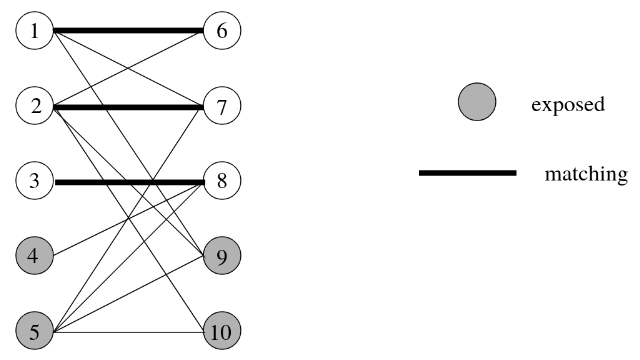
\includegraphics[width=0.6\textwidth]{Immagini/matching_example.png}
    \caption{Example of a perfect matching in a bipartite graph.}
    \label{fig:matching_example}
\end{figure}

The problem of finding a minimum weight perfect matching in a bipartite graph is a well-known problem in combinatorial optimization. The problem can be formulated as follows: given a weighted bipartite graph $G = (V, E)$, where $V = V_1 \cup V_2$ and $V_1 \cap V_2 = \emptyset$, find a perfect matching $M$ such that the sum of the weights of the edges in $M$ is minimized. The weight of a matching is the sum of the weights of the edges in the matching. The weight of an edge $e = (u, v)$ is denoted by $w(e)$. This problem is also called \textbf{the assignment problem}.

\subsection{Problem formulation}
The problem of finding a minimum weight perfect matching in a bipartite graph can be formulated as an integer linear program (ILP), i.e.an optimization problem in which the variables are restricted to integer values and the constraints and the objective function are linear as a function of these variables. Given a matching $M$, let $x$ be its incidence vector where $x_{ij} = 1$ if edge $(i, j)$ is in the matching, and $x_{ij} = 0$ otherwise. Then, the problem can be formulated as follows:

\begin{equation}
    \begin{aligned}
        \text{minimize} \quad & \sum_{(i, j) \in E} w_{ij} x_{ij} \\
        \text{subject to} \quad & \sum_{j \in V_2} x_{ij} = 1, \quad \forall i \in V_1 \\
        & \sum_{i \in V_1} x_{ij} = 1, \quad \forall j \in V_2 \\
        & x_{ij} \in \{0, 1\}, \quad \forall (i, j) \in E
    \end{aligned}
\end{equation}

Notice that any solution to this integer program corresponds to a matching and therefore this is a valid formulation of the minimum weight perfect matching problem in bipartite graphs.

The linear program relaxation of the above integer program is as follows:

\begin{equation}
    \begin{aligned}
        \text{minimize} \quad & \sum_{(i, j) \in E} w_{ij} x_{ij} \\
        \text{subject to} \quad & \sum_{j \in V_2} x_{ij} = 1, \quad \forall i \in V_1 \\
        & \sum_{i \in V_1} x_{ij} = 1, \quad \forall j \in V_2 \\
        & 0 \leq x_{ij} \leq 1, \quad \forall (i, j) \in E
    \end{aligned}
\end{equation}

The set of feasible solutions to the constraints in (P) forms a polytope. When optimizing a linear constraint over a polytope, the optimum will be achieved at one of the "corners" or extreme points of the polytope. An extreme point $x$ of a set $Q$ is an element $x \in Q$ that cannot be expressed as $\lambda y + (1 - \lambda) z$ with $0 < \lambda < 1$, $y, z \in Q$, and $y \neq z$. (This concept will be formalized and discussed in more detail when we cover polyhedral theory.)

In general, even if all the coefficients of the constraint matrix in a linear program are either 0 or 1, the extreme points of a linear program are not guaranteed to have all coordinates integral. This is not surprising since the general integer programming problem is NP-hard, while linear programming is solvable in polynomial time. Consequently, there is no guarantee that the value $Z_{IP}$ of an integer program is equal to the value $Z_{LP}$ of its LP relaxation. However, since the integer program is more constrained than the relaxation, we always have $Z_{IP} \geq Z_{LP}$, implying that $Z_{LP}$ is a lower bound on $Z_{IP}$ for a minimization problem. Moreover, if an optimal solution to a linear programming relaxation is integral, then it must also be an optimal solution to the integer program.

In our problem, the constraint matrix has a special form that lead to the following result: 

\begin{teorema}
    Any extreme point of ($P$) is a $0-1$ vector and, hence, is the incidence vector of a perfect matching.
\end{teorema}

Consequently, the polytope

\begin{equation}
    \begin{aligned}
        P = \{ x: & \sum_{j \in V_2} x_{ij} = 1, \quad \forall i \in V_1, \\
        & \sum_{i \in V_1} x_{ij} = 1, \quad \forall j \in V_2, \\
        & 0 \leq x_{ij} \leq 1, \quad \forall (i, j) \in E \}
    \end{aligned}
\end{equation}

is called the bipartite perfect matching polytope. 

\section{Solutions to the problem}
There are several algorithms to solve the problem of finding a minimum weight perfect matching in a bipartite graph. The first algorithm to solve this problem was proposed by Kuhn in 1955 \cite{kuhn1955hungarian}. The algorithm is based on the Hungarian method, which is a combinatorial optimization algorithm that solves the assignment problem in polynomial time. In the original paper the complexity of the algorithm was $O(n^4)$, but later Dinic and Kronrod \cite{dinic1969algorithm} showed that the algorithm can be implemented in $O(n^3)$ time.

The Hungarian method is a powerful algorithm, however, the algorithm is not very intuitive and can be difficult to implement. In recent years, several other algorithms have been proposed to solve the problem of finding a minimum weight perfect matching in a bipartite graph. In 1970, Edmonds and Karp \cite{edmonds1972theoretical} proposed an algorithm that solves the problem in $O(nm + n^2 \log n)$ time. In 1989 Gabow and Tarjan \cite{gabow1989faster} proposed an algorithm that solves the problem in $O(\sqrt{n}m \log(nW))$ time,  where $n,m$ and $W$ denote the number of vertices, number of edges, and largest magnitude of a cost; costs are assumed to be integral. The algorithms work by scaling. Lastly, in 2009, Sankowski and Piotr \cite{sankowski2009maximum} introduced a randomized algorithm that solves the problem in $O(Wn^w)$ time, where $w$ is the exponent of matrix multiplication, and $W$ is the highest edge weight in the graph.

\section{Implementation}
In this section, we will present an implementation of the Gabow and Tarjan algorithm to solve the problem of finding a minimum weight perfect matching in a bipartite graph. The algorithm is based on scaling and is a generalization of the Hungarian method. The algorithm works by scaling the edge weights and then finding a perfect matching in the scaled graph. 

\newpage
\
\newpage
\chapter{Tree Compression Scheme} \label{chp:project_overview}
As introduced in the first chapter, the primary goal of this thesis is to develop a novel tree compression scheme that effectively leverages repetitive structures within the input trie. The proposed algorithm is designed to identify and compactly represent these recurring patterns, thereby improving compression performance, particularly for highly repetitive tries. This chapter provides an overview of the proposed compression scheme.

\section{Compression Scheme Pipeline}
The overall pipeline of our proposed method is outlined in Algorithm~\ref{alg:pipeline}. It takes an input trie $T$ and a width parameter $p$ and produces a compressed, $p$--sortable automaton.
\begin{algorithm}[H]
\caption{$\textsc{CompressTrie}(T,p)$}
\label{alg:pipeline}
\begin{algorithmic}[1]
\Require Input trie $T$, width integer parameter $p$
\Ensure A compressed, $p$--sortable automaton $\mathcal{A}$
    \State $V_{sorted} = \textsc{PathSort}(T)$ 
    \State $N[1,\dots,|Q|] = \text{RevuzMinimization}(T)$
    \State $G_{bipartite} = \text{ConstructMWPBMInstance}(V_{sorted}, N, p)$
    \State $M = \text{SolveMWPBM}(G_{bipartite})$ 
    \State $C[1,\dots,p] = \text{ExtractChainsFromMatching}(M, V_{sorted})$ 
    \State $\mathcal{A} = \text{CollapseChains}(C, N)$ 
    \State \Return $\mathcal{A}$
\end{algorithmic}
\end{algorithm}

The first step of the pipeline (line 2) establishes a total order on the nodes of the trie. This is achieved by sorting the nodes co--lexicographically using the \textbf{Path Sort} algorithm, which we described in \cref{alg:pathSort}. This sorting is fundamental, as it arranges the nodes in the order required for a Wheeler automaton.

Next, the algorithm identifies which nodes are candidates for merging (line 3). This is done by partitioning the nodes into equivalence classes based on the structure of the subtrees rooted at each node. Two nodes are in the same class if and only if their subtrees are isomorphic. This is equivalent to computing the Myhill--Nerode equivalence classes for the finite language accepted by the trie, a process we adapt from Revuz's algorithm for minimizing acyclic DFAs (\cref{alg:minimization-ADFA}).

The core of the algorithm lies in lines 4 and 5, where we solve the \textbf{String Partitioning Problem}. The input to this problem is the string formed by concatenating the Myhill--Nerode classes of the sorted nodes. As detailed in \cref{sec:reduction_to_mwpbm}, we reduce this problem to finding a Minimum Weight Perfect Bipartite Matching (MWPBM). A bipartite graph is constructed where the weight of each edge corresponds to the cost of placing two characters adjacently in a subsequence. By finding a perfect matching with minimum weight using standard algorithms (\cref{sec:mwpbm_solutions}), we can reconstruct a partition of the string into $p$ subsequences that minimizes the total number of runs, thereby maximizing compression.

Finally, the DAG compressed automaton is constructed (line 6). The algorithm iterates through each of the $p$ subsequences and ``collapses'' any consecutive sequence of nodes belonging to the same Myhill--Nerode equivalence class into a single state. This compression, which we describe in \cref{sec:collapsing}, produces the final $p$--sortable automaton, which can then be indexed for efficient querying (\cref{sec:indexing}).

\begin{example}[Compression pipeline] \label{ex:string_example}
    In our running example, we begin with the tree shown in \cref{fig:mn-compressed-tree}. Each node in this tree is labeled with its corresponding Myhill--Nerode equivalence class, as determined in \cref{ex:ADFA_minimization}. By traversing the nodes in co--lexicographic order, we construct a string $S$ where each character represents the Myhill--Nerode equivalence class of a node:
    \[
        S = \text{ABCDDCBDDDD}
    \]
    This string $S$ then becomes the input to the String Partitioning Problem (see \cref{def:string_partitioning_problem}), where the objective is to partition $S$ into $p$ subsequences while minimizing the total number of runs.

    % First figure - Original tree
    \begin{figure}[H]
        \centering
        \begin{tikzpicture}[
    level distance=1.5cm,
    sibling distance=3cm,
    state/.style={circle, draw, minimum size=7mm},
    accepting/.style={circle, draw, double, minimum size=7mm},
    edge from parent/.style={draw, -latex},
    level 1/.style={sibling distance=4cm},
    level 2/.style={sibling distance=2.5cm},
    level 3/.style={sibling distance=2cm}
    ]

\node[state] (a) {A}
    child {node[state] (b) {B} 
    child {node[state] (d) {C}
        child {node[accepting] (h) {D}}
        child {node[accepting] (i) {D}}
    }
    child {node[accepting] (e) {D}}
    }
    child {node[state] (c) {B}
    child {node[state] (f) {C}
        child {node[accepting] (l) {D}}
        child {node[accepting] (m) {D}}
    }
    child {node[accepting] (g) {D}}
    };
\end{tikzpicture}
        \caption{Tree ADFA of \cref{fig:example_ADFA}, with each node labeled with its equivalence class.}
        \label{fig:mn-compressed-tree}
    \end{figure}

    Given $p = 2$, one way to partition the string is $C = [\text{ABCDCBD}, \text{DDDD}]$, which is clearly suboptimal as the total number of runs is $runs(C) = 7 + 1 = 8$.
    An optimal solution would be $C' = [\text{ABCCB}, \text{DDDDDD}]$, since $runs(C') = 4 + 1 = 5$ is the minimum number of runs for the partition of $S$ into two chains.
    
\end{example}
\section{Reducing the Chains-Division Problem to the Assignment Problem}
In this section, we will show how we can reduce the problem of finding the optimal partition of the nodes of a labeled tree $T$ given their equivalence classes into $p$ chains to the Minimum Weight Perfect Bipartite Matching problem (see \cref{def:mwpbm}). We define $\equivset$ as the set of equivalence classes of the nodes of $T$, and $t$ as the number of nodes of the tree. This reduction will allow us to solve the problem in polynomial time, as shown in the previous chapter.

In particular, we show that, given a tree $T$ and the number of chains $p$, we can construct a bipartite graph $G = (V, E)$ in which a perfect matching (\cref{def:matching}) always exists. In turn, a perfect matching with minimum weight enables us to retrieve the optimal partition of the nodes in $T$ into $p$ chains, such that the run-length encoding of each chain is minimized.

Then, we will show how to optimize the reduction by introducing some constraints that will allow us to reduce the number of edges in the bipartite graph, and we will also show how to move from the Minimum Weight Perfect Bipartite Matching problem to the more studied Maximum Weight Perfect Bipartite Matching problem without losing generality.

\subsection{Chains-Division Problem Definition}
It is essential to begin by defining the problem we aim to solve.

\begin{definition}[Chains-Division Problem] \label{def:problem_def}
    Given a labeled tree $T$, the equivalence classes $\equivset$, the stable order of the nodes in $T$ according to the upward path $\pi$ as defined in \cref{def:node_informations}, and an integer parameter $p \in [2, t]$, find the optimal partition of the nodes of $T$ into $p$ chains such that the run-length encoding of each chain is minimized.
\end{definition}

Let's give a formal definition of run-length encoding.
\begin{definition}[Run length encoding]
    Given a sequence $S = \{s_1, s_2, \dots, s_n\}$, the run length encoding of $S$ is the sequence $R = \{r_1, r_2, \dots, r_m\}$ where $r_i$ is the number of times the element $s_i$ is repeated in $S$.
\end{definition}

It allows us to represent the sequence $S$ in a more compact way. 

\begin{example}
    Let $S = \{A, A, B, B, B, C, C, A, A\}$. The run-length encoding of $S$ would be $R = \{(A, 2), (B, 3), (C, 2), (A, 2)\}$. The length of the RLE, which is the value we want to minimize, is $|R|=4$.
\end{example}

So, we aim to divide the nodes of the tree into $p$ chains such that the run-length encoding of the chains is minimized, meaning we want to reduce the number of distinct equivalence classes in each chain. Follows the definition of a chain.

\begin{definition}[Chains] \label{def:chains}
    Given a tree $T$, a chain $C$ is a sequence of nodes $C = \{c_1, c_2, \dots, c_m\}$ such that $C\subseteq V$. Additionally, each node of $T$ belongs to exactly one chain, and the nodes in the chain are ordered according to the upward path $\pi$ (as defined in \cref{def:node_informations}) of each node $c_i$.
\end{definition}

Note that, following the XBWT definition, two sibling nodes are comparable. The stable sorting algorithm respects the original sibling order, meaning the node that appears first among its siblings in a pre-order traversal will also come first in the sorted sequence.

\begin{example}[Chains-Division Problem]
    Consider a tree $T$ with 7 nodes having the following equivalence classes: $E = \{A, B, A, C, A, B, B\}$, where the nodes are ordered according to their upward paths. Let's say we want to divide these nodes into $p = 2$ chains.
    
    \textbf{Non-optimal division:} If we divide the nodes into chains $C_1 = \{A, B, A, C\}$ and $C_2 = \{A, B, B\}$, the run-length encoding would be:
    \begin{itemize}
        \item $C_1$: $(A,1), (B,1), (A,1), (C,1)$ - requiring 4 pairs
        \item $C_2$: $(A,1), (B,2)$ - requiring 2 pairs
    \end{itemize}
    Total RLE cost: $4 + 2 = 6$
    
    \textbf{Optimal division:} A better division would be $C_1 = \{A, A, A\}$ and $C_2 = \{B, C, B, B\}$, with run-length encoding:
    \begin{itemize}
        \item $C_1$: $(A,3)$ - requiring 1 pair
        \item $C_2$: $(B,1), (C,1), (B,2)$ - requiring 3 pairs
    \end{itemize}
    Total RLE cost: $1 + 3 = 4$
    
    This example demonstrates how grouping nodes of the same equivalence class in chains minimizes the total run-length encoding cost. The optimal solution can be found by reducing this problem to the \textsc{MWPBM} problem as described in this chapter.
\end{example}

\begin{comment}
\subsection{Reduction idea}
The intuition behind the reduction is the following: given a tree $T$ and the number of chains $p$, we can construct a bipartite graph $G = (V, E)$ in which a perfect matching (\cref{def:matching}) always exists. In turn, a perfect matching with minimum weight enables us to retrieve the optimal partition of the nodes in $T$ into $p$ chains, such that the run-length encoding of each chain is minimized.

In the following sections we will show how to construct the bipartite graph $G$ and proof that $G$ constructed as defined in \cref{def:bip_construction} always allows to find a perfect matching and the weight of the matching is the minimum run length encoding of the optimal partition of the nodes of $T$ into $p$ chains.

\alessio{Introduci il bipartite graph con troppa cattiveria :). Prima abbiamo parlato di alberi, adesso subito di grafi bipartiti. La soluzione con grafo bipartito è quella che hai voluto seguire tu, quindi dovresti introdurla più come una scelta implementativa, che come un dato di fatto. In breve, dovresti dimostrare qua che Chains-Div. si riduce al MWBGP, quindi sarebbe da girare un attimo l'ordine: Se abbiamo un grafo con un perfect matching allora possiamo ridurre il problema -> creiamo un grafo in questo modo -> contiene un perfect matching -> possiamo sempre fare la riduzione.} \davide{Ho aggiunto un paragrafo introduttivo.. può andare o intendevi proprio girare tutta la dimostrazione?}
\alessio{Se l'esistenza perfect matching è sufficiente a fare la riduzione, secondo me è meglio girare l'ordine delle dimostrazioni. Altrimenti, se per la riduzione ti servono le proprietà specifiche del grafo che hai creato allora va bene questo ordine. Pensandoci, puoi riportare questa discussione nell'intrduzione della sezione 6.2, mettendo qualcosa tipo ``In particular we show that, given a tree $T$ and the number of chains $p$, we can construct a bipartite ...'' tra i due paragrafi che ci sono già. (occhio alle frasi troppo lunghe).}
\end{comment}

\subsection{Bipartite Graph Construction}
Now, we will show how to construct a bipartite graph that allows us to solve the \textsc{CHAINS-DIVISION} problem.

\begin{definition}[Bipartite graph construction] \label{def:bip_construction}
    Let $T$ be a tree with $t$ nodes, and $p$ the number of chains we want to partition the nodes into. Let $\equivset$ be the set of equivalence classes of the nodes of $T$. We can construct a bipartite graph $G = (V, E)$ such that vertices are divided in two disjoint sets $V = V_1 \cup V_2$ in the following way:
    \begin{itemize}[leftmargin=25pt]
        \item $V_1$ contains $t + p$ nodes composed by $p$ source nodes $s_1, s_2, \dots, s_p$ (referred to collectively as $\sourceset$) followed by the $t$ elements (referred to collectively as $\treeset{1}$) of $\equivset$. The nodes in $V_1$ follow a strict ordering $s_1 \prec s_2 \prec \dots \prec s_p \prec u_1 \prec u_2 \prec \dots \prec u_t$, where $u_i$ are the tree nodes ordered according to the upward path $\pi$ as defined in \cref{def:node_informations}.
        \item $V_2$ contains $t + p$ nodes composed by the $t$ elements (referred to collectively as $\treeset{2}$) of $\equivset$ followed by $p$ destination nodes $d_1, d_2, \dots, d_p$ (referred to collectively as $\destset$). The nodes in $V_2$ follow a strict ordering $v_1 \prec v_2 \prec \dots \prec v_t \prec d_1 \prec d_2 \prec \dots \prec d_p$, where $v_i$ are the tree nodes ordered according to the upward path $\pi$ as defined in \cref{def:node_informations}.
    \end{itemize}

    Then the edges of the graph $G$ are constructed in the following way:
    \begin{enumerate}[leftmargin=25pt]
        \item The $\sourceset$ nodes are connected to the first $p$ nodes with distinct equivalence class in $V_2$, with weight $1$.
        \item Let $u_i \in \treeset{1}$. We define $\equivsetfunc{u_i}$ as the equivalence class of node $u_i$. For each node $u_i$, we construct the following edges:
        
        - For the first $p$ nodes $v_j \in \treeset{2}$ such that $j > i$ and $\equivsetfunc{v_j} \neq \equivsetfunc{u_i}$, we add an edge $(u_i, v_j)$ with weight $1$. If there are fewer than $p$ nodes in $V_2$ with distinct equivalence classes, we stop earlier.

        - Let $v_k \in \treeset{2}$ be the first node in the ordering such that $k > i$ and $\equivsetfunc{v_k} \neq \equivsetfunc{u_i}$, we add an edge $(u_i, v_k)$ with weight $0$. If such a node does not exist, we add $p$ edges $(u_i, d_j)$ with weight $0$ for each $j = 1, 2, \ldots, p$, where $d_j \in \destset$.
    \end{enumerate}
\end{definition}

Notice that it is important to consider the order of the nodes of the two sets $V_1$ and $V_2$ as stated in the definition, because we will need to connect the source nodes to the destination nodes in a way that will allow us to find the optimal partition of the nodes of the tree. An example of the node structure is shown in \cref{ex:reduction_vertices}.

Notice also that when we talk about the same $\treeset{1}$ node placed in $\treeset{2}$, we are referring to the corresponding node in $\treeset{2}$ that derives from the same node in the original tree $T$ since the nodes of the tree are ordered in both sets $\treeset{1}$ and $\treeset{2}$. In \cref{fig:bipartite_structure,fig:reduction_small_examples,fig:reduction_example}, the node's correspondence is achieved by putting the two nodes at the same level.
\begin{example}[Vertices] \label{ex:reduction_vertices}
    This example illustrates the structure of the bipartite graph vertices for the tree shown in \cref{fig:original_tree}. The nodes in this tree are labeled by their equivalence classes obtained from the minimization of the corresponding ADFA in \cref{ex:ADFA_minimization}. Our goal is to partition the tree's nodes into $p=2$ chains. The nodes of the tree are ordered according to \cref{alg:pathSort}, the order is the following: 
    \[
        a \prec b \prec d \prec h \prec l \prec f \prec c \prec e \prec i \prec m \prec g
    \]

    \cref{fig:bipartite_structure} shows the corresponding bipartite graph. The graph is composed of:
    \begin{itemize}
        \item Two source nodes ($s_1, s_2$) on the left, representing the start of each chain.
        \item Two sets of tree nodes, representing the partitions $\treeset{1}$ (left column) and $\treeset{2}$ (right column). These nodes are ordered based on the \texttt{pathSort} algorithm. The labels (A, B, C, D) correspond to the equivalence classes from the original tree.
        \item Two destination nodes ($d_1, d_2$) on the right, representing the end of each chain.
    \end{itemize}

    % First figure - Original tree
    \begin{figure}[H]
        \centering
        \begin{tikzpicture}[
            level distance=1.5cm,
            sibling distance=3cm,
            state/.style={circle, draw, minimum size=7mm},
            accepting/.style={circle, draw, double, minimum size=7mm},
            edge from parent/.style={draw, -latex},
            level 1/.style={sibling distance=4cm},
            level 2/.style={sibling distance=2.5cm},
            level 3/.style={sibling distance=2cm}
            ]
        
        \node[state] (a) {A}
            child {node[state] (b) {B} 
            child {node[state] (d) {C}
                child {node[accepting] (h) {D}}
                child {node[accepting] (i) {D}}
            }
            child {node[accepting] (e) {D}}
            }
            child {node[state] (c) {B}
            child {node[state] (f) {C}
                child {node[accepting] (l) {D}}
                child {node[accepting] (m) {D}}
            }
            child {node[accepting] (g) {D}}
            };
        \end{tikzpicture}
        \caption{Tree ADFA of \cref{fig:example_ADFA}. Each node is labeled with its equivalence class.}
        \label{fig:original_tree}
    \end{figure}
    
    % Second figure - Bipartite graph structure
    \begin{figure}[H]
        \centering
        \tikzset{main/.style = {draw, circle, thick, minimum size=8mm, inner sep=0pt}}
        \begin{tikzpicture}[node distance=10mm]
            % Define node styles
            \tikzstyle{main} = [circle, draw, minimum size=0.8cm, font=\small]
            \tikzstyle{source} = [circle, draw, minimum size=0.8cm, font=\small, fill=green!20]
            \tikzstyle{dest} = [circle, draw, minimum size=0.8cm, font=\small, fill=blue!20]
            
            % Source nodes (left column, green background)
            \node[source] (s1) {$s_1$};
            \node[source] (s2) [below of=s1] {$s_2$};
            
            % Tree nodes (left column, red border)
            \node[main] (t1) [below of=s2, yshift=-0.3cm] {A};
            \node[main] (t2) [below of=t1] {B};
            \node[main] (t3) [below of=t2] {C};
            \node[main] (t4) [below of=t3] {D};
            \node[main] (t5) [below of=t4] {D};
            \node[main] (t6) [below of=t5] {C};
            \node[main] (t7) [below of=t6] {B};
            \node[main] (t8) [below of=t7] {D};
            \node[main] (t9) [below of=t8] {D};
            \node[main] (t10) [below of=t9] {D};
            \node[main] (t11) [below of=t10] {D};
            
            % Tree nodes (right column, red border)
            \node[main] (r1) [right of=t1, xshift=3cm] {A};
            \node[main] (r2) [below of=r1] {B};
            \node[main] (r3) [below of=r2] {C};
            \node[main] (r4) [below of=r3] {D};
            \node[main] (r5) [below of=r4] {D};
            \node[main] (r6) [below of=r5] {C};
            \node[main] (r7) [below of=r6] {B};
            \node[main] (r8) [below of=r7] {D};
            \node[main] (r9) [below of=r8] {D};
            \node[main] (r10) [below of=r9] {D};
            \node[main] (r11) [below of=r10] {D};
            
            % Destination nodes (right column, blue background)
            \node[dest] (d1) [below of=r11, yshift=-0.3cm] {$d_1$};
            \node[dest] (d2) [below of=d1] {$d_2$};
            
            % Draw colored rectangles around groups
            % Green rectangle for source nodes
            \draw[green, thick, rounded corners] ([xshift=-0.4cm,yshift=0.25cm]s1.north west) rectangle ([xshift=0.4cm,yshift=-0.25cm]s2.south east);
            
            % Red rectangle for left tree nodes
            \draw[red, thick, rounded corners] ([xshift=-0.4cm,yshift=0.4cm]t1.north west) rectangle ([xshift=0.4cm,yshift=-0.4cm]t11.south east);
            
            % Red rectangle for right tree nodes
            \draw[red, thick, rounded corners] ([xshift=-0.4cm,yshift=0.4cm]r1.north west) rectangle ([xshift=0.4cm,yshift=-0.4cm]r11.south east);
            
            % Blue rectangle for destination nodes
            \draw[blue, thick, rounded corners] ([xshift=-0.4cm,yshift=0.25cm]d1.north west) rectangle ([xshift=0.4cm,yshift=-0.25cm]d2.south east);
            
            % Add labels
            \node[green!100, font=\small\bfseries] at ([xshift=1.5cm]s1.east) {Source};
            \node[green!100, font=\small\bfseries] at ([xshift=1.5cm]s2.east) {nodes};
            
            \node[red, font=\small\bfseries] at ([xshift=1.5cm]t6.east) {Tree};
            \node[red, font=\small\bfseries] at ([xshift=1.5cm]t7.east) {nodes};
            
            \node[blue, font=\small\bfseries] at ([xshift=-1.5cm]d1.west) {Destination};
            \node[blue, font=\small\bfseries] at ([xshift=-1.5cm]d2.west) {nodes};
            
            % Add "Corresponding tree node" label with arrow
            \draw[<->, thick] (t1.east) -- (r1.west);
            \node[font=\small] at ([xshift=0cm,yshift=-0.25cm]$(t1)!0.5!(r1)$) {Corresponding};
            \node[font=\small] at ([xshift=0cm,yshift=-0.7cm]$(t1)!0.5!(r1)$) {tree node};
            
        \end{tikzpicture}
        \caption{Corresponding bipartite graph structure for the tree in \cref{fig:original_tree} with $p=2$. The nodes are ordered from top to bottom using \cref{alg:pathSort}.}
        \label{fig:bipartite_structure}
    \end{figure}
\end{example}

\begin{example}[Edges]
    Let's see a small example for each case. Consider $p=2$. In \cref{fig:reduction_small_examples}-(a), there is an example for the sources' edges. As stated before, for each source, $p$ edges with weight $1$ are created and connected to the first $p$ nodes with distinct equivalence classes in $\treeset{2}$.

    In \cref{fig:reduction_small_examples}-(b), there is an example for the tree nodes' edges. For each node in $\treeset{1}$, edges with weight $1$ are created and connected to the first $p$ nodes with distinct equivalence class in $\treeset{2}$ after the corresponding node in $\treeset{2}$ (coming after the node itself in the ordering), and edges with weight $0$ are created and connected to the first node with the same class in $\treeset{2}$ after the corresponding node in $\treeset{2}$. As we can see from the image, we consider the first node in $\treeset{1}$ labelled $A$ that is connected to the node labelled $B$ with weight $1$, and to the node labelled $C$ with weight $1$, and to the second node labelled $A$ in $\treeset{2}$ with weight $0$.

    Lastly, in \cref{fig:reduction_small_examples}-(c) there is an example for the destination nodes' edges. We start by considering the node in $\treeset{1}$ that is labeled $A$, which is connected to a node labeled $B$ with weight $1$. Then, since there is no node with the same class in $\treeset{2}$, we connect it to the destination nodes $d_1$ and $d_2$ with weight $0$. The same is done for the second node in $\treeset{1}$ that is labelled $B$ since no nodes are coming after it in the order; it is connected to the destination nodes $d_1$ and $d_2$ with weight $0$.

    \begin{figure}[H]
        \centering
        \tikzset{main/.style = {draw, circle, thick, minimum size=8mm, inner sep=0pt}}
        \begin{subfigure}[b]{0.3\textwidth}
            \centering
            \begin{tikzpicture}[node distance=10mm, auto=center]
                \tikzstyle{main} = [circle, draw, minimum size=0.8cm, font=\small]
                \tikzstyle{source} = [circle, draw, minimum size=0.8cm, font=\small, fill=green!20]
                \tikzstyle{dest} = [circle, draw, minimum size=0.8cm, font=\small, fill=blue!20]
                
                % Left column (sources)
                \node[source] (1s) {$s_1$};
                \node[source] (2s) [below of=1s] {$s_2$};
                \node[main] (3s) [below of=2s] {A};
                \node[right=0cm of 3s] {$\cdots$};
                \node[main] (4s) [below of=3s] {A};
                \node[right=0cm of 4s] {$\cdots$};
                \node[main] (5s) [below of=4s] {B};
                \node[right=0cm of 5s] {$\cdots$};
                \node (dots_s) [below of=5s] {\vdots}; % Vertical dots

                % Right column (destinations)
                \node[main] (1d) [right=2.5cm of 3s] {A};
                \node[main] (2d) [below of=1d] {A};
                \node[left=0cm of 2d] {$\cdots$};
                \node[main] (3d) [below of=2d] {B};
                \node[left=0cm of 3d] {$\cdots$};
                \node (dots_d) [below of=3d] {\vdots}; % Vertical dots

                % Arrows
                \draw[red, ->] (1s) -- (1d);
                \draw[red, ->] (1s) -- (3d);
                \draw[red, ->] (2s) -- (1d);
                \draw[red, ->] (2s) -- (3d);
            \end{tikzpicture}
            \caption{}
            \label{fig:sub1}
        \end{subfigure}
        \hfill % Space between subfigures
        \tikzset{main/.style = {draw, circle, thick, minimum size=8mm, inner sep=0pt}}
        \begin{subfigure}[b]{0.3\textwidth}
            \centering
            \begin{tikzpicture}[node distance=10mm, auto=center]
                \tikzstyle{main} = [circle, draw, minimum size=0.8cm, font=\small]
                \tikzstyle{source} = [circle, draw, minimum size=0.8cm, font=\small, fill=green!20]
                \tikzstyle{dest} = [circle, draw, minimum size=0.8cm, font=\small, fill=blue!20]

                % Left column (tree nodes)
                \node (dots_s_top) {\vdots};
                \node[main] (3s) [below of=dots_s_top] {A};
                \node[main] (4s) [below of=3s] {B};
                \node[right=0cm of 4s] {$\cdots$};
                \node[main] (5s) [below of=4s] {A};
                \node[right=0cm of 5s] {$\cdots$};
                \node[main] (6s) [below of=5s] {C};
                \node[right=0cm of 6s] {$\cdots$};
                \node (dots_s_bottom) [below of=6s] {\vdots};

                % Right column (destinations)
                \node (dots_d_top) [right=2.5cm of dots_s_top] {\vdots};
                \node[main] (1d) [below of=dots_d_top] {A};
                \node[left=0cm of 1d] {$\cdots$};
                \node[main] (2d) [below of=1d] {B};
                \node[left=0cm of 2d] {$\cdots$};
                \node[main] (3d) [below of=2d] {A};
                \node[left=0cm of 3d] {$\cdots$};
                \node[main] (4d) [below of=3d] {C};
                \node[left=0cm of 4d] {$\cdots$};
                \node (dots_d_bottom) [below of=4d] {\vdots};

                % Arrows
                \draw[red, ->] (3s) -- (2d);
                \draw[red, ->] (3s) -- (4d);
                \draw[green, ->] (3s) -- (3d);
            \end{tikzpicture}
            \caption{}
            \label{fig:sub2}
        \end{subfigure}
        \hfill % Space between subfigures
        \tikzset{main/.style = {draw, circle, thick, minimum size=8mm, inner sep=0pt}}
        \begin{subfigure}[b]{0.3\textwidth}
            \centering
            \begin{tikzpicture}[node distance=10mm, auto=center]
                \tikzstyle{main} = [circle, draw, minimum size=0.8cm, font=\small]
                \tikzstyle{source} = [circle, draw, minimum size=0.8cm, font=\small, fill=green!20]
                \tikzstyle{dest} = [circle, draw, minimum size=0.8cm, font=\small, fill=blue!20]

                % Left column (original destinations)
                \node (dots_s_top) {\vdots};
                \node[main] (7s) [below of=dots_s_top] {A};
                \node[main] (9s) [below of=7s] {B};

                % Right column (bipartite graph destinations)
                \node (dots_d_top) [right=2.5cm of dots_s_top] {\vdots};
                \node[main] (5d) [below of=dots_d_top] {A};
                \node[left=0cm of 5d] {$\cdots$};
                \node[main] (6d) [below of=5d] {B};
                \node[left=0cm of 6d] {$\cdots$};
                \node[dest] (8d) [below of=6d] {$d_1$};
                \node[left=0cm of 8d] {$\cdots$};
                \node[dest] (9d) [below of=8d] {$d_2$};
                \node[left=0cm of 9d] {$\cdots$};

                % Arrows
                \draw[red, ->] (7s) -- (6d);
                \draw[green, ->] (7s) -- (8d);
                \draw[green, ->] (7s) -- (9d);
                \draw[green, ->] (9s) -- (8d);
                \draw[green, ->] (9s) -- (9d);
            \end{tikzpicture}
            \caption{}
            \label{fig:sub3}
        \end{subfigure}

        \caption[Examples of reduction to a bipartite graph]{Examples of the connection construction in the bipartite graph for $p=2$, showing the cases for source nodes $\sourceset$ (a), internal tree nodes $\treeset{1}$ and $\treeset{2}$ (b), and destination nodes $\destset$ (c). Red arrows indicate edges with weight 1, while green arrows indicate edges with weight 0.}
        \label{fig:reduction_small_examples}
    \end{figure}
\end{example}


Before we present the proof of the correctness of the reduction, let us state the following theorem regarding the number of edges in the bipartite graph resulting from \cref{def:bip_construction}. This theorem is essential for understanding the complexity of the final algorithm employed to solve the \textsc{MWPBM} problem and so, the \textsc{CHAIN-DIVISION} problem.

\begin{theorem}[Bipartite graph properties]
    The bipartite graph $G$ constructed as stated in \cref{def:bip_construction} has $2t + 2p$ nodes and $O(t (p + 1) + p^2 + tp)$ edges.
\end{theorem}

\begin{proof}
    The $O(t (p + 1))$ edges come from the tree nodes, the $O(p^2)$ edges come from the sources since each source node is connected to $p$ nodes, and the $O(tp)$ edges come from the destination nodes since in the worst case we have $t$ distinct equivalence classes, which means that all the nodes are connected to the destination nodes. 
\end{proof}

\subsection{Proof of Correctness}
In this section, we present the proof of the correctness of the reduction introduced in the previous sections. Let us start by stating the following lemmas.

\begin{comment}
\begin{lemma} \label{lemma:all_destinations}
    Exactly $|\equivset|$ nodes of the set $\treeset{1}$ are connected to all the destination nodes $d_i \in \destset$ with weight $0$.
\end{lemma}

\begin{proof}
    As outlined in \cref{def:bip_construction}, the destination nodes $d_i \in V_2$ are connected to nodes $u_i \in \treeset{1}$ with weight $0$ iff for all $v_j \in \treeset{2}$ such that $j > i$, $\equivsetfunc{v_j} \neq \equivsetfunc{u_i}$, i.e. $u_i$ is the last of its class in the ordering. Consequently, there are exactly $|\equivset|$ nodes in $\treeset{1}$ that are last representatives of their class in the ordering.
\end{proof}
\end{comment}

\begin{lemma} \label{lemma:optimal_cost}
    The optimal solution of an instance $\mathcal{I}$ of the \textit{CHAINS-DIVISION} problem for a tree $T$ is always greater than or equal to $|\equivset|$.
\end{lemma}

\begin{proof}
    To minimize the run-length encoding of the chains, we note that the minimum cost of a chain is $1$. Consequently, the optimal cost of the \textit{CHAINS-DIVISION} problem for the tree $T$ is always greater than or equal to the cardinality of the set of equivalence classes $\equivset$ This is because if we partition them into $p = |\equivset|$ chains, the cost will be equal to $|\equivset|$, since each chain contains only nodes belonging to the same class. Conversely, if we partition them into $p < |\equivset|$ chains, the cost will be greater than or equal to $|\equivset|$ since we will need to include at least two nodes from different classes within a single chain.
\end{proof}

\begin{claim} \label{claim:p_less_than_E}
    The solutions for the \textit{CHAINS-DIVISION} problem for the instances where the number $p$ of chains is greater than $|\equivset|$ are not better than the solutions for the instances where $p \leq |\equivset|$.
\end{claim}

\begin{proof}
    The proof builds upon \cref{lemma:optimal_cost}. If we use a number of chains $p > |\equivset|$, we would have at least $p - |\equivset|$ empty chains, since there are only $|\equivset|$ non-empty equivalence classes of nodes to partition. As the minimum cost for any chain is 1, these empty chains contribute to the total cost. An optimal arrangement would involve $|\equivset|$ chains, each containing nodes from a single equivalence class, costing $|\equivset|$, and $p - |\equivset|$ empty chains, each costing 1. The total cost would be $|\equivset| + (p - |\equivset|) = p$. Since $p > |\equivset|$, this cost is greater than the optimal cost of $|\equivset|$ achievable with $p = |\equivset|$ chains. Therefore, any solution with $p > |\equivset|$ is suboptimal.
\end{proof}

Therefore, for the proof of the reduction, we will only consider instances of the problem where $p < |\equivset|$, as they do not present a trivial solution.

\begin{lemma} \label{lemma:greater_nodes}
    Given a bipartite graph $G$ constructed as stated in \cref{def:bip_construction}, for each node $u_i \in$ $\treeset{1}$ it is impossible for $u_i$ to be connected to a node $v_j \in \treeset{2}$, such that $j \leq i$ in the order of the nodes.
\end{lemma}

\begin{proof}
    The proof comes from the construction of $G$ (\cref{def:bip_construction}) where the nodes of $\treeset{1}$ are always connected to the nodes of $\treeset{2}$ coming after them.
\end{proof}

\begin{lemma} \label{claim:node_connectivity}
    In the bipartite graph $G$ constructed as per \cref{def:bip_construction}, for every node $u \in \treeset{1}$ $|N(\{u\})| \geq 1$.
\end{lemma}
In other words, every node in $V_1$ is connected to at least another node in $V_2$.
\begin{proof}
    Let $u_i \in \treeset{1}$ be an arbitrary node. We analyze the construction of its outgoing edges based on \cref{def:bip_construction}. There are two mutually exclusive cases for $u_i$:
    \begin{enumerate}[leftmargin=25pt]
        \item There exists at least one node $v_k \in \treeset{2}$ with $k > i$ that has the same equivalence class as $u_i$, i.e., $\equivsetfunc{v_k} = \equivsetfunc{u_i}$. In this case, the construction specifies that an edge is added between $u_i$ and the first such node $v_k$. This guarantees $u_i$ has at least one neighbor.
        \item There are no nodes $v_k \in \treeset{2}$ with $k > i$ that share the same equivalence class as $u_i$. This occurs when $u_i$ is the last node of its equivalence class in the specified ordering. In this scenario, the construction adds $p$ edges from $u_i$ to each of the destination nodes $d_j \in \destset$. Since $p \geq 2$, $u_i$ is connected to at least two nodes.
    \end{enumerate}
    In either case, any node $u_i \in \treeset{1}$ is guaranteed to have at least one outgoing edge. Therefore, its neighborhood is non-empty.
\end{proof}

\begin{lemma} \label{lemma:distinct_neighborhoods}
    For any pair of distinct nodes $u_i, u_j \in \treeset{1}$ such that $u_i \prec u_j$, $N(\{u_i\}) \not\subseteq N(\{u_j\})$.
\end{lemma}
\begin{proof}
    By \cref{claim:node_connectivity}, the set of neighbors $N(\{u_i\})$ and $N(\{u_j\})$ are non-empty. We will show that $N(\{u_i\}) \not\subseteq N(\{u_j\})$. 
    
    By construction, $u_i$ is connected to $v_{i+1}$. This holds whether $v_{i+1}$ is the next node in the same equivalence class or one of the first $p$ nodes in a different class. Thus, $v_{i+1} \in N(\{u_i\})$.

    From \cref{lemma:greater_nodes}, any neighbor $v_k$ of $u_j$ must have $k > j$. Since $i < j$, we have $i+1 \leq j$.
    This means $v_{i+1}$ cannot be a neighbor of $u_j$, as $i + 1 < k$. Therefore, $v_{i+1} \in N(\{u_i\})$ but $v_{i+1} \notin N(\{u_j\})$, which proves that $N(\{u_i\}) \not\subseteq N(\{u_j\})$.
\end{proof}

\begin{lemma} \label{lemma:distinct_neighborhoods_2}
    For any pair of distinct nodes $u_i, u_j \in \treeset{1}$ such that $u_i \prec u_j$ and $u_j$ is not the last node of its equivalence class in the order, then $N(\{u_j\}) \not\subseteq N(\{u_i\})$.
\end{lemma}
\begin{proof}
    Since $u_j$ is not the last node of its equivalence class, by construction, it must be connected to the first node $v_k \in \treeset{2}$ with $k > j$ such that $\equivsetfunc{v_k} = \equivsetfunc{u_j}$. Therefore, $v_k \in N(\{u_j\})$.

    By construction, it follows that $u_i$ cannot be connected to $v_k$. This is due to the existence of another node $v_l \in \treeset{2}$ with $i < l \leq j$, such that $\equivsetfunc{v_l} = \equivsetfunc{u_k}$. Consequently, we conclude that $v_k \notin N(\{u_i\})$, as the edges of $u_i$ connect to nodes in $\treeset{2}$, all of which belong to distinct classes.

    In summary, we have identified a node $v_k$ that is included in $N({u_j})$ but excluded from $N({u_i})$, thus proving that $N({u_j}) \not\subseteq N({u_i})$.
\end{proof}

\begin{comment}
\alessio{Non so se sia abbastanza questo claim, forse andrebbe dimostrato in entrambe le direzioni, quindi $N(\{u_i\}) \not\subseteq N(\{u_j\})$ e $N(\{u_j\}) \not\subseteq N(\{u_i\})$. In pratica la dimostrazione è la stessa ma va spiegata bene. A questo punto no so se il Lemma 4 serva, dato che deriva fa questa proprietà. Quindi in pratica il nodo sopra sarà connesso a nodi sopra il nodo sotto, mentre il nodo sotto sarà connesso ad altri nodi più sotto.
Dimostrando questo, puoi dire che ogni nodo aggiunge sempre almeno un nodo in più a $N(W)$, che sarà quindi almeno uguale a $|W|$. Occhio che però questo vale solo per i nodi che non sono gli ultimi della loro classe.} \davide{dovrei aver dimostrato le due strade e aggiunto nel lemma dell'esistenza del matching il caso in cui $u_j$ è l'ultimo nodo della sua classe.}
\begin{claim} \label{claim:prev_not_subset}
    For any pair of distinct nodes $u_i, u_j \in \treeset{1}$ with $i < j$, then we have that $N(\{u_i\}) \not\subseteq N(\{u_j\})$.
\end{claim}
\begin{proof}
    This is a direct consequence of the proof of \cref{lemma:distinct_neighborhoods}. In its proof, we showed that for any pair of nodes $u_i, u_j$ with $i < j$, there exists a neighbor $v_k \in N(\{u_i\})$ such that $k \leq j$. By \cref{lemma:greater_nodes}, any neighbor of $u_j$ must have an index greater than $j$. Therefore, $v_k$ cannot be a neighbor of $u_j$, which implies that $N(\{u_i\})$ cannot be a subset of $N(\{u_j\})$.
\end{proof}
\end{comment}

\begin{lemma} \label{lemma:matching_existence}
    For every possible instance of the \textit{CHAINS-DIVISION} problem, a perfect matching exists in the bipartite graph G constructed as specified in \cref{def:bip_construction}.
\end{lemma}
\begin{proof}
    The proof comes from the construction of the bipartite graph $G$ and from \cref{thm:halls_marriage_theorem}. We are going to prove that $G$ satisfies Hall's condition (see \cref{thm:halls_marriage_theorem}) and so, since by construction $|V_1| = |V_2|$, a perfect matching for $G$ exists.

    To verify Hall's condition, we need to prove that for any subset $W \subseteq V_1$ we have that $|N(W)| \geq |W|$, where $N(W)$ is the neighborhood of $W$ (\cref{def:neighborhood}). We have the following cases:
    \begin{enumerate}[leftmargin=25pt]
        \item $W \subseteq \sourceset$: Let $W$ be a subset of $S$ of size $k$. By construction, every source node $s_i \in \sourceset$ is connected to the same set of $p$ nodes in $V_2$, which are the first $p$ nodes with distinct equivalence classes in the ordering. Therefore, for any non-empty $W \subseteq \sourceset$, the neighborhood $N(W)$ consists of exactly these $p$ nodes, so $|N(W)| = p$. From \cref{lemma:optimal_cost} and \cref{claim:p_less_than_E}, we only consider instances where $p \leq |\equivset|$, ensuring that at least $p$ such nodes exist. Since $|\sourceset|=p$, we have $|W| = k \leq p$. Thus, $|N(W)| \geq |W|$.
        
        \item $W \subseteq \treeset{1}$: Let $W = \{u_{i_1}, \dots, u_{i_k}\} \subseteq \treeset{1}$ with $i_1 < i_2 < \dots < i_k$. We analyze two subcases:

        \textbf{Case A: No node in $W$ is the last of its class.}
        By \cref{lemma:distinct_neighborhoods,lemma:distinct_neighborhoods_2}, for any two nodes $u_a, u_b \in W$ with $a < b$, we have both $N(\{u_a\}) \not\subseteq N(\{u_b\})$ and $N(\{u_b\}) \not\subseteq N(\{u_a\})$. This implies that each node in $W$ contributes at least one unique neighbor to the total neighborhood $N(W)$. Therefore, $|N(W)| \geq |W|$.

        \textbf{Case B: At least one node in $W$ is the last of its class.}
        Let $u_{j} \in W$ be a node that is the last of its equivalence class. By construction, $u_{j}$ is connected to all $p$ destination nodes $\destset$, which means $\destset \subseteq N(W)$ and thus $|N(W)| \geq p$.

        For such a node $u_j$, its neighborhood $N(\{u_j\})$ may be a subset of $N(\{u_a\})$ for some $u_a \in W$ with $a < j$, since \cref{lemma:distinct_neighborhoods_2} does not apply. However, the reverse is not true, as \cref{lemma:distinct_neighborhoods} guarantees $N(\{u_a\}) \not\subseteq N(\{u_j\})$. This asymmetry ensures that $N(\{u_a\})$ always contributes at least one neighbor not present in $N(\{u_j\})$. This property, combined with the fact that all nodes that are last of their class are connected to the $p$ destination nodes, is sufficient to guarantee that $|N(W)| \ge |W|$ since $p \geq 2$.

        In both cases, Hall's condition $|N(W)| \geq |W|$ is satisfied for any $W \subseteq \treeset{1}$.
        
        \item $W=W_S \cup W_U$, where $W_S \subseteq \sourceset, W_U \subseteq \treeset{1}$: The neighborhood of $W_S$ consists of $p$ nodes, as established in case 1 ($W \subseteq \sourceset$). By \cref{lemma:greater_nodes}, the neighbors of any node in $W_U$ appear later in the node ordering than the node itself. Since all nodes in $\treeset{1}$ are ordered after the source nodes, the neighbors of $W_U$ are distinct from the neighbors of $W_S$. Specifically, $N(W_S)$ consists of the first $p$ nodes with distinct equivalence classes.
        
        We now analyze two subcases for nodes in $W_U$: If $W_U$ contains a node $u_i \in \treeset{1}$ that is not the last of its equivalence class, then there exists at least one node $v_j \in \treeset{2}$ with $i < j$ and $\equivsetfunc{u_i} = \equivsetfunc{v_j}$ that is connected to $u_i$ but not to any source node. This contributes additional neighbors to $N(W)$, ensuring $|N(W)| \geq |W|$.
        If $W_U$ contains a node $u_i \in \treeset{1}$ that is the last of its equivalence class, then by construction, $u_i$ is connected to all destination nodes. This guarantees $|N(W)| \geq |W|$.
        
        In both subcases, Hall's condition $|N(W)| \geq |W|$ is satisfied.
    \end{enumerate}
\end{proof}

\begin{comment}
    \begin{proof}
        The proof comes from the construction of the bipartite graph $G$ and from \cref{thm:perfect_matching_existence}. We are going to prove that the bipartite graph $G$ constructed as stated in \cref{def:bip_construction} has a Tutte matrix (\cref{def:tutte_matrix}) with determinant different from $0$ and so a perfect matching for $G$ exists.

        We know that an $n \times n$ matrix $M$ has $Det(M) \neq 0$ if and only if it has full rank ($rank(M) = n$), or equivalently if it has $n$ linearly independent rows or columns. We can see that the bipartite graph $G$ has $2t + 2p$ nodes and $O(t (p + 1) + p^2 + tp)$ edges, and so the Tutte matrix of $G$ will have $2t + 2p$ rows and $2t + 2p$ columns. The columns of $M$ are all independent since each node of $G$ in $V_1$ is connected only to nodes in $V_2$ that are greater than $u$ in the ordering. Also, each node is connected to at least one node in $V_2$ and at most $p + 1$ distinct nodes with distinct class in $V_2$. Those conditions on the edges are sufficient to get a full rank matrix and so a perfect matching for $G$ exists.
    \end{proof}

    In \cref{fig:tutte_matrix_ex}, the Tutte matrix for the bipartite graph in \cref{fig:reduction_example}-(a) is shown.

    \begin{figure}
        \centering
        \[
        \begin{array}{c|ccccccccc}
                & \text{1} & \text{2} & \text{1} & \text{3} & \text{1} & \text{2} & \text{2} & \text{$d_1$} & \text{$d_2$} \\
            \hline
            \text{$s_1$} & 1 & 1 & 0 & 0 & 0 & 0 & 0 & 0 & 0 \\
            \text{$s_2$} & 1 & 1 & 0 & 0 & 0 & 0 & 0 & 0 & 0 \\
            \text{1}     & 0 & 1 & 1 & 1 & 0 & 0 & 0 & 0 & 0 \\
            \text{2}     & 0 & 0 & 1 & 1 & 0 & 1 & 0 & 0 & 0 \\
            \text{1}     & 0 & 0 & 0 & 1 & 1 & 1 & 0 & 0 & 0 \\
            \text{3}     & 0 & 0 & 0 & 0 & 1 & 1 & 0 & 1 & 1 \\
            \text{1}     & 0 & 0 & 0 & 0 & 0 & 1 & 0 & 1 & 1 \\
            \text{2}     & 0 & 0 & 0 & 0 & 0 & 0 & 1 & 0 & 0 \\
            \text{2}     & 0 & 0 & 0 & 0 & 0 & 0 & 0 & 1 & 1 \\
        \end{array}
        \]
        \caption[Tutte matrix example]{Example of a Tutte matrix for a bipartite graph in \cref{fig:reduction_example}-(a). As we can see the matrix has full rank and so a perfect matching exists.}
        \label{fig:tutte_matrix_ex}
    \end{figure}
\end{comment}

We can now prove the correctness of the reduction. Consider a perfect matching $M$ in $G$. Therefore, $|V_1|=|V_2|$ and $M$ is perfect, every node in $V_1$ is matched to exactly one node in $V_2$, and vice versa. The matching $M$ consists of $t+p$ edges. Due to the construction of $G$ (\cref{def:bip_construction}) and \cref{lemma:greater_nodes} (a node $u_i \in \treeset{1}$ only connect to a node $v_j \in \treeset{2}$ with $i < j$ or to destination nodes $\destset$), the matching $M$ naturally decomposes into $p$ paths starting from the source nodes $s_1, \dots, s_p$ and ending at the destination nodes $d_1, \dots, d_p$. Each path traverses a sequence of nodes corresponding to the nodes of the original tree $T$.
Specifically, a path starting at $s_i$ will match it to a node $u_{a} \in \treeset{2}$. Then, the corresponding node of $u_{a} \in \treeset{1}$ can be matched to a node $u_{b} \in \treeset{2}$ (where $b > a$). This continues until a node $u_{x} \in \treeset{1}$ is matched to a destination node $d_k \in \destset$. This forms a sequence $s_i \rightarrow u_{a} \rightarrow u_{b} \rightarrow \dots \rightarrow u_{x} \rightarrow d_k$. Following this technique, we will retrieve all the optimal chains from the solution of the \textsc{MWPBM} problem.

\begin{example}
    Consider the example in \cref{fig:example_bipartite_read}. It shows a bipartite graph constructed from a tree (not shown) and a perfect matching within it. The solid arrows represent the edges of the perfect matching, where an edge $(u, v)$ signifies that node $v$ follows node $u$ in a path. The dashed arrows link the segments of the paths by connecting a node's representation in $V_2$ to its corresponding representation in $V_1$.

    The matching partitions the nodes into two distinct paths, differentiated by color:
    \begin{itemize}
        \item \textbf{Path 1 (red):} Starting from source $s_1$, the matching edge $(s_1, A)$ leads to the first node, $A$. The dashed arrow from this node in $V_2$ points to the same node $A$ in $V_1$, which is then matched with another $A$ in $V_2$. Following the next dashed arrow to the final $A$ in $V_1$, we see it is matched with the destination $d_1$. This sequence traces the path $s_1 \to A \to A \to d_1$ leading to the chain $C_{red}=\{A,A\}$.
        \item \textbf{Path 2 (blue):} Starting from source $s_2$, the matching edge $(s_2, B)$ leads to node $B$. The dashed arrow connects to the next $B$ in $V_1$, which is matched with destination $d_2$, tracing the path $s_2 \to B \to d_2$ leading to the chain $C_{blue}=\{B\}$.
    \end{itemize}
    This demonstrates how a perfect matching in the bipartite graph yields a valid partition of the original tree's nodes into paths from sources to destinations.
    \begin{figure}[H]
        \centering
        \tikzset{main/.style = {draw, circle, thick, minimum size=8mm, inner sep=0pt}}
        \begin{tikzpicture}[node distance=10mm, auto=center]
            \tikzstyle{main} = [circle, draw, minimum size=0.8cm, font=\small]
            \tikzstyle{source} = [circle, draw, minimum size=0.8cm, font=\small, fill=green!20]
            \tikzstyle{dest} = [circle, draw, minimum size=0.8cm, font=\small, fill=blue!20]

            % Left column (original destinations)
            \node[source] (1s) {$s_1$};
            \node[source] (2s) [below of=1s] {$s_2$};
            \node[main] (7s) [below of=2s] {A};
            \node[main] (8s) [below of=7s] {A};
            \node[main] (9s) [below of=8s] {B};

            % Right column (bipartite graph destinations)
            \node[main] (5d) [right=2.5cm of 7s] {A};
            \node[main] (7d) [below of=5d] {A};
            \node[main] (6d) [below of=7d] {B};
            \node[dest] (8d) [below of=6d] {$d_1$};
            \node[dest] (9d) [below of=8d] {$d_2$};

            % Arrows
            \draw[red, ->] (1s) -- (5d);
            \draw[red, ->] (7s) -- (7d);
            \draw[red, ->] (8s) -- (8d);
            \draw[red, dashed, ->] (5d) -- (7s);
            \draw[red, dashed, ->] (7d) -- (8s);

            \draw[blue, ->] (2s) -- (6d);
            \draw[blue, ->] (9s) -- (9d);
            \draw[blue, dashed, ->] (6d) -- (9s);
        \end{tikzpicture}
        \caption{An example of a perfect matching (solid lines) in the constructed bipartite graph. The matching defines a partition into two paths (red and blue), which are traced by following the solid and dashed arrows.}
        \label{fig:example_bipartite_read}
    \end{figure}
\end{example}

\begin{theorem}
    An optimal solution of an instance $\mathcal I$ with $p \leq |\equivset|$ of the \textsc{CHAINS-DIVISION} problem (\cref{def:problem_def}) is equivalent to an optimal solution of the \textsc{MWPBM} problem (\cref{def:mwpbm}) for the instance $r(\mathcal I)$ where $r: \mathcal{I}_{CHAINS-DIVISION} \rightarrow \mathcal{I}_{MWPBM}$ is the reduction function that maps an instance of the CHAINS-DIVISION problem to an instance of the MWPBM problem for a bipartite graph $G$ constructed as stated in \cref{def:bip_construction}.
\end{theorem}

\begin{proof}
    Let $\mathcal{I} = (T, \equivset, p)$ be an instance of the \textsc{CHAINS-DIVISION} problem, where $T$ is a tree with $t$ nodes, $\equivset$ is the set of equivalence classes, and $p$ is the target number of chains. We assume $p \leq |\equivset|$, per \cref{claim:p_less_than_E}. Let $G = r(\mathcal{I})$ be the bipartite graph constructed according to \cref{def:bip_construction}. We will demonstrate a bijection between the set of valid chain partitions of $T$ and the set of perfect matchings in $G$, such that the cost of a partition equals the weight of its corresponding matching.

    First, we establish the existence of a perfect matching. By construction, the graph $G$ is bipartite with partitions $V_1$ and $V_2$ such that $|V_1| = |V_2| = t+p$. \cref{lemma:matching_existence} ensures that a perfect matching exists in $G$.

    Let $\mathcal{P} = \{C_1, \dots, C_p\}$ be a valid partition of the nodes of $T$ into $p$ chains. We can construct a perfect matching $M_\mathcal{P}$ in $G$ as follows:  For each chain $C_k = [u_{1}, \dots, u_{m_k}]$, we construct a path in $G$: match $s_k$ to $u_{1} \in \treeset{2}$. Then match $u_{i} \in \treeset{1}$ to $u_{i+1} \in \treeset{2}$ for $i=1, \dots, m_k-1$. Finally, match $u_{m_k} \in \treeset{1}$ to one of the available destination nodes $d_j \in \destset$. Since we have $p$ chains and $p$ source/destination nodes, and every tree node is in exactly one chain, this process uses all $t+p$ nodes in $V_1$ and $V_2$, forming a perfect matching. The weight of this matching is given by:
    \begin{align*}
        W(M_\mathcal{P}) &= \sum_{(u,v) \in M_\mathcal{P}} w(u,v) \\
        &= p + |\{ (u_i, u_j) \in M_\mathcal{P} \mid u_i \in \treeset{1}, u_j \in \treeset{2}, \equivsetfunc{u_i} \neq \equivsetfunc{u_j} \}|
    \end{align*}
    where $p$ represents the contribution from the source nodes $s_i$, as each source node must be connected with weight 1 to start a chain. A class change occurs exactly when a path in the matching uses a weight-1 edge between tree nodes.
    Therefore, $W(M)$ is exactly equal to the RLE cost of the partition defined by the matching $M_\mathcal{P}$.

    Conversely, let $M$ be a perfect matching in $G$. The structure of $G$ ensures that $M$ consists of $p$ disjoint paths starting from source nodes $\{s_1, \dots, s_p\}$ and ending at destination nodes $\{d_1, \dots, d_p\}$. Each path defines an ordered chain of nodes from $T$. By \cref{lemma:greater_nodes}, the node order within these chains is consistent with the original node ordering $\pi$. Thus, $M$ maps to a valid partition of $T$. The cost of this partition is equal to $W(M)$.

    Since there is a cost-preserving bijection between the set of all valid partitions and the set of all perfect matchings, an optimal solution to one problem corresponds to an optimal solution to the other. Therefore, finding a minimum weight perfect matching in $G$ is equivalent to solving the \textsc{CHAINS-DIVISION} problem for $T$.
\end{proof}

\begin{example} \label{ex:reduction_ex}
    Consider the example in \cref{fig:reduction_example} where we have the bipartite graph for the tree in \cref{fig:original_tree} and $p = 2$. In \cref{fig:reduction_example}-(a) we have the resulting bipartite graph, and in \cref{fig:reduction_example}-(b) we have one of the possible minimum perfect matchings for the graph in (a) having weight $5$. At the end we can see that the optimal partition of the nodes of the tree $T$ is $C_1 = \{A,C,C,B\}$ and $C_2 = \{B,D,D,D,D,D,D\}$ with a total cost of $5$, this can be obtained starting from the sources and by following the edges of the nodes, jumping to the corresponding node in $V_1$ and following the edges again until we reach the destination nodes.

    \begin{figure}[H]
        \centering
        \begin{tabular}{cc}
            \tikzset{main/.style = {draw, circle, thick, minimum size=8mm, inner sep=0pt}}
            \begin{tikzpicture}[node distance={10mm}, thick, auto=center, main/.style = {draw, circle}]
                \tikzstyle{main} = [circle, draw, minimum size=0.8cm, font=\small]
                \tikzstyle{source} = [circle, draw, minimum size=0.8cm, font=\small, fill=green!20]
                \tikzstyle{dest} = [circle, draw, minimum size=0.8cm, font=\small, fill=blue!20]

                % Source nodes (left column, green background)
                \node[source] (s1) {$s_1$};
                \node[source] (s2) [below of=s1] {$s_2$};
                
                % Tree nodes (left column, red border)
                \node[main] (t1) [below of=s2] {A};
                \node[main] (t2) [below of=t1] {B};
                \node[main] (t3) [below of=t2] {C};
                \node[main] (t4) [below of=t3] {D};
                \node[main] (t5) [below of=t4] {D};
                \node[main] (t6) [below of=t5] {C};
                \node[main] (t7) [below of=t6] {B};
                \node[main] (t8) [below of=t7] {D};
                \node[main] (t9) [below of=t8] {D};
                \node[main] (t10) [below of=t9] {D};
                \node[main] (t11) [below of=t10] {D};
                
                % Tree nodes (right column, red border)
                \node[main] (r1) [right of=t1, xshift=3cm] {A};
                \node[main] (r2) [below of=r1] {B};
                \node[main] (r3) [below of=r2] {C};
                \node[main] (r4) [below of=r3] {D};
                \node[main] (r5) [below of=r4] {D};
                \node[main] (r6) [below of=r5] {C};
                \node[main] (r7) [below of=r6] {B};
                \node[main] (r8) [below of=r7] {D};
                \node[main] (r9) [below of=r8] {D};
                \node[main] (r10) [below of=r9] {D};
                \node[main] (r11) [below of=r10] {D};
                
                % Destination nodes (right column, blue background)
                \node[dest] (d1) [below of=r11] {$d_1$};
                \node[dest] (d2) [below of=d1] {$d_2$};
                
                \draw[red, ->] (s1) -- (r1);
                \draw[red, ->] (s1) -- (r2);
                \draw[red, ->] (s2) -- (r1);
                \draw[red, ->] (s2) -- (r2);
                \draw[red, ->] (t1) -- (r2);
                \draw[red, ->] (t1) -- (r3);
                \draw[green, ->] (t1) -- (d1);
                \draw[green, ->] (t1) -- (d2);
                \draw[red, ->] (t2) -- (r3);
                \draw[red, ->] (t2) -- (r4);
                \draw[green, ->] (t2) -- (r7);
                \draw[red, ->] (t3) -- (r4);
                \draw[red, ->] (t3) -- (r7);
                \draw[green, ->] (t3) -- (r6);
                \draw[green, ->] (t4) -- (r5);
                \draw[red, ->] (t4) -- (r6);
                \draw[red, ->] (t4) -- (r7);
                \draw[red, ->] (t5) -- (r6);
                \draw[red, ->] (t5) -- (r7);
                \draw[green, ->] (t5) -- (r8);
                \draw[red, ->] (t6) -- (r7);
                \draw[red, ->] (t6) -- (r8);
                \draw[green, ->] (t6) -- (d1);
                \draw[green, ->] (t6) -- (d2);
                \draw[red, ->] (t7) -- (r8);
                \draw[green, ->] (t7) -- (d1);
                \draw[green, ->] (t7) -- (d2);
                \draw[green, ->] (t8) -- (r9);
                \draw[green, ->] (t9) -- (r10);
                \draw[green, ->] (t10) -- (r11);
                \draw[green, ->] (t11) -- (d1);
                \draw[green, ->] (t11) -- (d2);
            \end{tikzpicture} &
            \tikzset{main/.style = {draw, circle, thick, minimum size=8mm, inner sep=0pt}}
            \begin{tikzpicture}[node distance={10mm}, thick, auto=center, main/.style = {draw, circle}]
                \tikzstyle{main} = [circle, draw, minimum size=0.8cm, font=\small]
                \tikzstyle{source} = [circle, draw, minimum size=0.8cm, font=\small, fill=green!20]
                \tikzstyle{dest} = [circle, draw, minimum size=0.8cm, font=\small, fill=blue!20]

                % Source nodes (left column, green background)
                \node[source] (s1) {$s_1$};
                \node[source] (s2) [below of=s1] {$s_2$};
                
                % Tree nodes (left column, red border)
                \node[main] (t1) [below of=s2] {A};
                \node[main] (t2) [below of=t1] {B};
                \node[main] (t3) [below of=t2] {C};
                \node[main] (t4) [below of=t3] {D};
                \node[main] (t5) [below of=t4] {D};
                \node[main] (t6) [below of=t5] {C};
                \node[main] (t7) [below of=t6] {B};
                \node[main] (t8) [below of=t7] {D};
                \node[main] (t9) [below of=t8] {D};
                \node[main] (t10) [below of=t9] {D};
                \node[main] (t11) [below of=t10] {D};
                
                % Tree nodes (right column, red border)
                \node[main] (r1) [right of=t1, xshift=3cm] {A};
                \node[main] (r2) [below of=r1] {B};
                \node[main] (r3) [below of=r2] {C};
                \node[main] (r4) [below of=r3] {D};
                \node[main] (r5) [below of=r4] {D};
                \node[main] (r6) [below of=r5] {C};
                \node[main] (r7) [below of=r6] {B};
                \node[main] (r8) [below of=r7] {D};
                \node[main] (r9) [below of=r8] {D};
                \node[main] (r10) [below of=r9] {D};
                \node[main] (r11) [below of=r10] {D};
                
                % Destination nodes (right column, blue background)
                \node[dest] (d1) [below of=r11] {$d_1$};
                \node[dest] (d2) [below of=d1] {$d_2$};
                
                \draw[red, ->] (s1) -- (r1);
                \draw[red, ->] (s2) -- (r2);
                \draw[red, ->] (t1) -- (r3);
                \draw[red, ->] (t2) -- (r4);
                \draw[green, ->] (t3) -- (r6);
                \draw[green, ->] (t4) -- (r5);
                \draw[green, ->] (t5) -- (r8);
                \draw[red, ->] (t6) -- (r7);
                \draw[green, ->] (t7) -- (d1);
                \draw[green, ->] (t8) -- (r9);
                \draw[green, ->] (t9) -- (r10);
                \draw[green, ->] (t10) -- (r11);
                \draw[green, ->] (t11) -- (d2);
            \end{tikzpicture} \\
        (a) & (b) \\
        \end{tabular}
        \caption[Reduction full example]{Example of a reduction for the tree in \cref{fig:original_tree}. In (a), we have the resulting bipartite graph constructed. In (b), we have the resulting perfect matching for the graph in (a). Green edges weigh $0$, while red edges weigh $1$.}
        \label{fig:reduction_example}
    \end{figure}
\end{example}

\subsection{Heuristics and Improvements}
Some changes can be made to the reduction in order to optimize it and to reduce the number of edges in the bipartite graph. Here are some of the improvements that can be made.
    
\begin{lemma}[Sources' edges optimization] \label{lemma:sources_optimization}
    The sources' edges can be optimized by connecting each source only to the smallest node in $\treeset{2}$ that is not connected to any other source.
\end{lemma}

\begin{proof}
    Since the source nodes are needed to distinguish the chains as starting points, we need that each source is connected to exactly one node in $\treeset{2}$. Having the sources connected to the first $p$ nodes with distinct equivalence classes in $\treeset{2}$ is not necessary since it allows us just to invert the chains starting from each source, and so it is redundant. 

    Moreover, Hall's condition $|N(W)| \geq |W|$ still holds for any subset $W \subseteq V_1$ in the optimized graph. This follows trivially from the fact that case 1 of \cref{lemma:matching_existence} still guarantees that $|N(W)| \geq |W|$ for any subset $W \subseteq \sourceset$.
\end{proof}

\begin{example}
    Consider the bipartite graph shown in \cref{fig:source_optimization}. The red solid arrows represent edges with weight 1, while the red dashed arrows represent edges that can be optimized away according to \cref{lemma:sources_optimization}.

    In this example, we can observe the application of the optimization rule:
    \begin{itemize}
        \item The first tree node $A$ has a solid edge to the first destination node $A$ and a dashed edge to destination node $B$ to be removed. This since source $s_1$ is already connected to node $A$.
        \item Similarly, the second source node $s_2$ has a dashed edge to the first destination node $A$, which can be removed because $s_1$ is already connected to node $A$ with the same weight.
    \end{itemize}

    After applying the optimization, only the solid edges remain, resulting in a reduced bipartite graph that maintains the same optimal matching cost while having fewer edges to consider during the matching algorithm.
    \begin{figure}[H]
        \centering
        \tikzset{main/.style = {draw, circle, thick, minimum size=8mm, inner sep=0pt}}
        \begin{tikzpicture}[node distance=10mm, auto=center]
            \tikzstyle{main} = [circle, draw, minimum size=0.8cm, font=\small]
            \tikzstyle{source} = [circle, draw, minimum size=0.8cm, font=\small, fill=green!20]
            \tikzstyle{dest} = [circle, draw, minimum size=0.8cm, font=\small, fill=blue!20]
            
            % Left column (sources)
            \node[source] (1s) {$s_1$};
            \node[source] (2s) [below of=1s] {$s_2$};
            \node[main] (3s) [below of=2s] {A};
            \node[right=0cm of 3s] {$\cdots$};
            \node[main] (4s) [below of=3s] {A};
            \node[right=0cm of 4s] {$\cdots$};
            \node[main] (5s) [below of=4s] {B};
            \node[right=0cm of 5s] {$\cdots$};
            \node (dots_s) [below of=5s] {\vdots}; % Vertical dots

            % Right column (destinations)
            \node[main] (1d) [right=2.5cm of 3s] {A};
            \node[main] (2d) [below of=1d] {A};
            \node[left=0cm of 2d] {$\cdots$};
            \node[main] (3d) [below of=2d] {B};
            \node[left=0cm of 3d] {$\cdots$};
            \node (dots_d) [below of=3d] {\vdots}; % Vertical dots

            % Arrows
            \draw[red, ->] (1s) -- (1d);
            \draw[red, dashed, ->] (1s) -- (3d);
            \draw[red, dashed, ->] (2s) -- (1d);
            \draw[red, ->] (2s) -- (3d);
        \end{tikzpicture}
        \caption{Bipartite graph after applying Sources' edges optimization. Dashed edges from the original graph have been removed according to \cref{lemma:sources_optimization}, reducing the number of edges while preserving optimality. Red edges have weight $1$.}
        \label{fig:source_optimization}
    \end{figure}
\end{example}

This will reduce the number of edges coming from the sources from $p^2$ to $p$.

\begin{lemma}[Tree nodes' edges optimization 1] \label{lemma:tree_optimization_1}
    The tree nodes' edges can be optimized by removing the edges of the nodes in $\treeset{1}$ that are connected to nodes in $\treeset{2}$ already linked to a source node in $V_1$.
\end{lemma}

\begin{proof}
    This optimization follows directly from \cref{lemma:sources_optimization}.
    From \cref{def:matching} we know that a matching $M \in E$ is a collection of edges such that every vertex of $V$ is incident to at most one edge of $M$. In other words, a matching is a set of edges such that no two edges share a common vertex. Given that, in all the solutions to the problem, all sources will be connected to exactly one node in $\treeset{2}$. Therefore, we can remove the edges of the nodes in $\treeset{1}$ that are connected to nodes in $\treeset{2}$ already linked to a source node in $V_1$ since they will not be part of the final matching.
\end{proof}

\begin{example}
    Consider the bipartite graph shown in \cref{fig:tree_optimization_1}. The red arrows represent edges with weight $1$, while green arrows represent edges with weight $0$. Dashed edges represent edges that can be optimized away according to \cref{lemma:tree_optimization_1}.

    In particular, in \cref{fig:tree_optimization_1}, we can observe that the dashed edge from the first node $A$ in $\treeset{1}$ can be optimized away since it is connected to $B$ in $\treeset{2}$, which is already linked to a source node in $V_1$.
    \begin{figure}[H]
        \tikzset{main/.style = {draw, circle, thick, minimum size=8mm, inner sep=0pt}}
        \centering
        \begin{tikzpicture}[node distance=10mm, auto=center]
            \tikzstyle{main} = [circle, draw, minimum size=0.8cm, font=\small]
            \tikzstyle{source} = [circle, draw, minimum size=0.8cm, font=\small, fill=green!20]
            \tikzstyle{dest} = [circle, draw, minimum size=0.8cm, font=\small, fill=blue!20]
            
            % Left column (sources)
            \node[source] (1s) {$s_1$};
            \node[source] (2s) [below of=1s] {$s_2$};
            \node[main] (3s) [below of=2s] {A};
            \node[main] (4s) [below of=3s] {A};
            \node[right=0cm of 4s] {$\cdots$};
            \node[main] (5s) [below of=4s] {B};
            \node[right=0cm of 5s] {$\cdots$};
            \node[main] (6s) [below of=5s] {C};
            \node[right=0cm of 6s] {$\cdots$};
            \node (dots_s) [below of=6s] {\vdots}; % Vertical dots

            % Right column (destinations)
            \node[main] (1d) [right=2.5cm of 3s] {A};
            \node[main] (2d) [below of=1d] {A};
            \node[main] (3d) [below of=2d] {B};
            \node[left=0cm of 3d] {$\cdots$};
            \node[main] (4d) [below of=3d] {C};
            \node[left=0cm of 4d] {$\cdots$};
            \node (dots_d) [below of=4d] {\vdots}; % Vertical dots

            % Arrows
            \draw[red, ->] (1s) -- (1d);
            \draw[red, ->] (2s) -- (3d);
            \draw[green, ->] (3s) -- (2d);
            \draw[red, ->, dashed] (3s) -- (3d);
            \draw[red, ->] (3s) -- (4d);

        \end{tikzpicture}
        \caption{Bipartite graph after applying tree nodes' edges optimization 1. Dashed edges from the original graph have been removed according to \cref{lemma:tree_optimization_1}, reducing the number of edges while preserving optimality. Red edges have weight $1$, while green edges have weight $0$.}
        \label{fig:tree_optimization_1}
    \end{figure}
\end{example}

This will reduce the number of edges by a factor of $p-1$.

\begin{lemma}[Tree nodes' edges optimization 2] \label{lemma:tree_optimization_2}
    Edges of nodes in $\treeset{1}$ can be optimized by removing the edges with weight $1$ starting from a node $u \in \treeset{1}$ to a node $v \in \treeset{2}$ if the node $u$ has another edge with weight $0$ connected to a node $z \in \treeset{2}$ such that $z \prec v$ in the ordering of the nodes.
\end{lemma}

\begin{proof}
    Let $M$ be any perfect matching. Suppose $M$ contains an edge $(u, v)$ that satisfies the conditions of the lemma, i.e., $u \in \treeset{1}$, $v \in \treeset{2}$, $w(u,v) = 1$, and there exists an edge $(u, z)$ with $w(u,z) = 0$ for some $z \in \treeset{2}$ with $z \prec v$.

    We will show that this edge $(u,v)$ is not necessary for an optimal solution. Since $M$ is a perfect matching, $z$ must be matched with some node $u' \in \treeset{1}$, so $(u',z) \in M$. Note that $u' \neq u$ and that $u' \prec z$ for \cref{lemma:greater_nodes}.

    Consider an alternative matching $M' = (M \setminus \{(u,v), (u',z)\}) \cup \{(u,z), (u'',v)\}$. This is a valid perfect matching where $u$ is matched with $z$, and $u'' \in \treeset{1}$ is matched with $v$. By construction and from \cref{lemma:greater_nodes} we know that $u \prec u' \preceq u'' \prec v$.
    
    The weight of this new matching is $W(M') = W(M) - w(u,v) - w(u',z) + w(u,z) + w(u'',v)$.
    By substituting the known weights $w(u,v)=1$ and $w(u,z)=0$, we get:
    $W(M') = W(M) - 1 - w(u',z) + 0 + w(u'',v) = W(M) + (w(u'',v) - w(u',z)) - 1$.

    The construction of the graph ensures that for any node $u'' \in \treeset{1}$, the cost of connecting to $v$ is either the same or one greater than connecting to a preceding node $z$. That is, $w(u'',v) - w(u',z) \in \{-1, 1\}$. This property arises from the problem reduction, where moving to a subsequent node in the ordering can at most increment the cost by one.
    
    Therefore, $w(u'',v) - w(u',z) \le 1$, which implies $W(M') \leq W(M)$. Thus, the edge $(u,v)$ can be removed from the graph without affecting the weight of the optimal solution.

    Finally, we need to prove that \cref{lemma:matching_existence} still holds. The proof follows from showing that the two fundamental neighborhood properties remain valid after edge removal:
    \begin{enumerate}[leftmargin=25pt]
        \item \cref{lemma:distinct_neighborhoods} remains valid because it relies on the fact that each node $u_i \in \treeset{1}$ is connected to $v_{i+1} \in \treeset{2}$. The edge $(u,v)$ we remove cannot be this critical edge $(u_i,v_{i+1})$ since, by our optimization condition, there exists a node $z \prec v$ connected to $u$ with weight 0; the edge $(u_i,v_{i+1})$ is always the first valid connection for $u_i$ in the ordering. Therefore, $v$ cannot be $v_{i+1}$ for the node $u$.
        \item \cref{lemma:distinct_neighborhoods_2} is preserved because it concerns edges between nodes of the same equivalence class. Our optimization only removes an edge when there exists a better alternative to a preceding node, meaning that the same-class connectivity pattern is unaffected by this edge removal.
        \item The edge removal does not affect source and destination nodes' connections, as we only remove tree node edges.
    \end{enumerate}

    Since both \cref{lemma:distinct_neighborhoods,lemma:distinct_neighborhoods_2} remain valid and the source and destination connectivity is preserved, all conditions required by \cref{lemma:matching_existence} continue to hold, ensuring the existence of a perfect matching in the optimized graph.

    \alessio{La questione è che: se da un nodo con valore 1 voglio connettermi ad un nodo con valore 3, ma prima c'è un altro nodo con valore 1, tanto vale pasó che comunque ci sarà un collegamento tra quello nuovo e li 3 (da dimostrare). In questo modo, prendendo quel nodo, il costo della mia catena aumenta di 0, quindi non peggiora, e il coto di un altra catena potrebbe non aumentare, quindi togliamo una scelta ovviamente errata.} \davide{ho provato a renderla più generale. così mi sembra funzionare}
\end{proof}

\begin{example}
    Consider the bipartite graph in \cref{fig:tree_optimization_2}. The red arrows represent edges with weight $1$, while green arrows represent edges with weight $0$. Dashed edges represent edges that can be optimized away according to \cref{lemma:tree_optimization_2}.

    In this case, we can observe the application of the optimization rule: The edge $(A, C)$ is removed from the graph, as it is not necessary for an optimal solution. This is because the node $A$ has another edge with weight $0$ connected to a node $B$ with $B \prec C$.
    \begin{figure}[H]
        \tikzset{main/.style = {draw, circle, thick, minimum size=8mm, inner sep=0pt}}
        \centering
        \begin{tikzpicture}[node distance=10mm, auto=center]
            \tikzstyle{main} = [circle, draw, minimum size=0.8cm, font=\small]
            \tikzstyle{source} = [circle, draw, minimum size=0.8cm, font=\small, fill=green!20]
            \tikzstyle{dest} = [circle, draw, minimum size=0.8cm, font=\small, fill=blue!20]

            % Left column (tree nodes)
            \node (dots_s_top) {\vdots};
            \node[main] (3s) [below of=dots_s_top] {A};
            \node[main] (4s) [below of=3s] {B};
            \node[right=0cm of 4s] {$\cdots$};
            \node[main] (5s) [below of=4s] {A};
            \node[right=0cm of 5s] {$\cdots$};
            \node[main] (6s) [below of=5s] {C};
            \node[right=0cm of 6s] {$\cdots$};
            \node (dots_s_bottom) [below of=6s] {\vdots};

            % Right column (destinations)
            \node (dots_d_top) [right=2.5cm of dots_s_top] {\vdots};
            \node[main] (1d) [below of=dots_d_top] {A};
            \node[left=0cm of 1d] {$\cdots$};
            \node[main] (2d) [below of=1d] {B};
            \node[left=0cm of 2d] {$\cdots$};
            \node[main] (3d) [below of=2d] {A};
            \node[left=0cm of 3d] {$\cdots$};
            \node[main] (4d) [below of=3d] {C};
            \node[left=0cm of 4d] {$\cdots$};
            \node (dots_d_bottom) [below of=4d] {\vdots};

            % Arrows
            \draw[red, ->] (3s) -- (2d);
            \draw[red, dashed, ->] (3s) -- (4d);
            \draw[green, ->] (3s) -- (3d);
        \end{tikzpicture}
        \caption{Bipartite graph after applying tree nodes' edges optimization 2. Dashed edges from the original graph have been removed according to \cref{lemma:tree_optimization_2}, reducing the number of edges while preserving optimality. Red edges have weight $1$, while green edges have weight $0$.}
        \label{fig:tree_optimization_2}
    \end{figure}
\end{example}

\begin{comment}
In \cref{fig:heuristics_example}-(b), we can see the resulting bipartite graph for the example shown in the previous section after the optimizations.

\begin{figure}[H]
    \centering
    \begin{tabular}{cc}
        \begin{tikzpicture}[node distance={10mm}, thick, auto=center, main/.style = {draw, circle}]
            \node[main] (1s) {$s_1$};
            \node[main] (2s) [below of=1s] {$s_2$};
            \node[main] (3s) [below of=2s] {$1$};
            \node[main] (4s) [below of=3s] {$2$};
            \node[main] (5s) [below of=4s] {$1$};
            \node[main] (6s) [below of=5s] {$3$};
            \node[main] (7s) [below of=6s] {$1$};
            \node[main] (8s) [below of=7s] {$2$};
            \node[main] (9s) [below of=8s] {$2$};
            \node[main] (1d) [right=3cm of 3s] {$1$};
            \node[main] (2d) [below of=1d] {$2$};
            \node[main] (3d) [below of=2d] {$1$};
            \node[main] (4d) [below of=3d] {$3$};
            \node[main] (5d) [below of=4d] {$1$};
            \node[main] (6d) [below of=5d] {$2$};
            \node[main] (7d) [below of=6d] {$2$};
            \node[main] (8d) [below of=7d] {$d_1$};
            \node[main] (9d) [below of=8d] {$d_2$};

            \draw[black, dashed, ->] (1s) -- (1d);
            \draw[green, dashed, ->] (1s) -- (2d);
            \draw[green, dashed, ->] (2s) -- (1d);
            \draw[black, dashed, ->] (2s) -- (2d);
            \draw[blue, dashed, ->] (3s) -- (2d);
            \draw[red, dashed, ->] (3s) -- (4d);
            \draw[black, ->] (3s) -- (3d);
            \draw[black, dashed, ->] (4s) -- (3d);
            \draw[black, dashed, ->] (4s) -- (4d);
            \draw[black, ->] (4s) -- (6d);
            \draw[black, dashed, ->] (5s) -- (4d);
            \draw[black, ->] (5s) -- (5d);
            \draw[red, dashed, ->] (5s) -- (6d);
            \draw[black, dashed, ->] (6s) -- (5d);
            \draw[black, dashed, ->] (6s) -- (6d);
            \draw[black, ->] (6s) -- (8d);
            \draw[black, ->] (6s) -- (9d);
            \draw[black, dashed, ->] (7s) -- (6d);
            \draw[black, ->] (7s) -- (8d);
            \draw[black, ->] (7s) -- (9d);
            \draw[black, ->] (8s) -- (7d);
            \draw[black, ->] (9s) -- (8d);
            \draw[black, ->] (9s) -- (9d);
        \end{tikzpicture} &
        \begin{tikzpicture}[node distance={10mm}, thick, auto=center, main/.style = {draw, circle}]
            \node[main] (1s) {$s_1$};
            \node[main] (2s) [below of=1s] {$s_2$};
            \node[main] (3s) [below of=2s] {$1$};
            \node[main] (4s) [below of=3s] {$2$};
            \node[main] (5s) [below of=4s] {$1$};
            \node[main] (6s) [below of=5s] {$3$};
            \node[main] (7s) [below of=6s] {$1$};
            \node[main] (8s) [below of=7s] {$2$};
            \node[main] (9s) [below of=8s] {$2$};
            \node[main] (1d) [right=3cm of 3s] {$1$};
            \node[main] (2d) [below of=1d] {$2$};
            \node[main] (3d) [below of=2d] {$1$};
            \node[main] (4d) [below of=3d] {$3$};
            \node[main] (5d) [below of=4d] {$1$};
            \node[main] (6d) [below of=5d] {$2$};
            \node[main] (7d) [below of=6d] {$2$};
            \node[main] (8d) [below of=7d] {$d_1$};
            \node[main] (9d) [below of=8d] {$d_2$};

            \draw[black, dashed, ->] (1s) -- (1d);
            \draw[black, dashed, ->] (2s) -- (2d);
            \draw[black, ->] (3s) -- (3d);
            \draw[black, dashed, ->] (4s) -- (3d);
            \draw[black, dashed, ->] (4s) -- (4d);
            \draw[black, ->] (4s) -- (6d);
            \draw[black, dashed, ->] (5s) -- (4d);
            \draw[black, ->] (5s) -- (5d);
            \draw[black, dashed, ->] (6s) -- (5d);
            \draw[black, dashed, ->] (6s) -- (6d);
            \draw[black, ->] (6s) -- (8d);
            \draw[black, ->] (6s) -- (9d);
            \draw[black, dashed, ->] (7s) -- (6d);
            \draw[black, ->] (7s) -- (8d);
            \draw[black, ->] (7s) -- (9d);
            \draw[black, ->] (8s) -- (7d);
            \draw[black, ->] (9s) -- (8d);
            \draw[black, ->] (9s) -- (9d);
        \end{tikzpicture} \\
    (a) & (b) \\
    \end{tabular}
    \caption[Reduction heuristics example]{Example of a reduction for the sorted nodes' equivalency classes $E = \{1,2,1,3,1,2,2\}$ applying also the heuristics shown. In (a), the edges removed are shown in green for \cref{lemma:sources_optimization}, blue for \cref{lemma:tree_optimization_1}, and red for \cref{lemma:tree_optimization_2}. In (b), we have the resulting bipartite graph after the heuristics are applied. Dashed edges weigh $1$, while solid edges weigh $0$. \alessio{Invertirei la notazione degli archi: dashed (semi-trasparente) logicamente ha peso 0, mentre solid (si vede bene) ha peso 1.}}
    \label{fig:heuristics_example}
\end{figure}
\end{comment}

\subsection{Moving to Maximum weight perfect bipartite matching}
In this section, we will discuss how to slightly modify the reduction process to move from a minimum weight perfect bipartite matching problem to a maximum weight perfect bipartite matching problem. This will be helpful in solving the problem more efficiently by using some known algorithms to solve the maximum weight perfect bipartite matching problem.

\begin{theorem}
    An optimal solution of an instance $\mathcal I$ with $p \leq |E|$ of the \textsc{CHAINS-DIVISION} problem is equivalent to an optimal solution of the Maximum Weight Perfect Bipartite Matching for the instance $r(\mathcal I)$ where $r: \mathcal{I}_{CHAINS-DIVISION} \rightarrow \mathcal{I}_{MWPBM}$ is the reduction function that maps an instance of the \textsc{CHAINS-DIVISION} problem to an instance of the Maximum Weight Perfect Bipartite Matching problem constructed as stated in \cref{def:bip_construction} but with inverted weights (weight $0$ becomes $1$ and weight $1$ becomes $0$).
\end{theorem}

\begin{proof}
    Let $M$ be a perfect matching in the bipartite graph $G$ constructed as stated in \cref{def:bip_construction}. Let $w(M)$ be the sum of the weights of the edges in the matching $M$. From the previous theorem, we know that the optimal solution of the \textsc{CHAINS-DIVISION} problem is equivalent to finding a perfect matching $M$ in $G$ that minimizes $w(M)$.

    Let $G'$ be a bipartite graph constructed as $G$ but with inverted weights (weight $0$ becomes $1$ and weight $1$ becomes $0$). Let $M'$ be a perfect matching in $G'$ and let $w'(M')$ be the sum of the weights of the edges in the matching $M'$. Let $k$ be the number of edges in the matching.

    We can see that for any matching $M$ in $G$:
    \[ w'(M) = k - w(M) \]

    This means that maximizing $w'(M)$ is equivalent to minimizing $w(M)$. Therefore, finding the maximum weight perfect matching in $G'$ is equivalent to finding the minimum weight perfect matching in $G$, which in turn is equivalent to finding the optimal solution of the \textsc{CHAINS-DIVISION} problem.
\end{proof}

\newpage
\
% \chapter{Wheeler Graphs}

\section{Definition of Wheeler Graph}

\begin{definition} \label{def_wheeler_graphs}
    A Wheeler graph $G=(V,E)$ is defined as a directed graph with labeled edges, equipped with a total order $<_{\pi}$ on the nodes in $V$, which satisfies the following three axioms:

    \begin{enumerate}[(i)]
        \item All vertices with in-degree $0$ must precede those with a greater in-degree in the ordering; \label{axiom_1}
    \suspend{enumerate}
    For every pair of edges $(u_1,v_1,k_1)$ and $(u_2,v_2,k_2)$:
    \resume{enumerate}[{[(i)]}]
        \item $k_1<k_2 \Rightarrow v_1<_{\pi}v_2$; \label{axiom_2}
        \item $(k_1=k_2) \wedge (u_1<_{\pi}u_2) \Rightarrow v_1\leq_{\pi}v_2$. \label{axiom_3}
    \end{enumerate}
\end{definition}

\section{Examples of Wheeler Graphs}
\begin{figure}[H]
    \centering
    \begin{tikzpicture}[node distance={25mm}, thick, auto=center, main/.style = {draw, circle}]
        \node[main] (1) {$x_1$};
        \node[main] (2) [below left of=1] {$x_2$};
        \node[main] (3) [below right of=1] {$x_3$};
        \node[main] (4) [below of=2] {$x_4$};
        \node[main] (5) [below of=3]{$x_5$};
        \draw[red, ->] (1) -- (3);
        \draw[red, ->] (1) -- (2);
        \draw[red, ->] (4) -- (3);
        \draw[red, ->] (5) -- (3);
        \draw[green, ->] (2) -- (5);
        \draw[blue, ->] (2) -- (4);
        \draw (4) edge[blue, loop left] (4);
    \end{tikzpicture}
    \caption[Example of a Wheeler Graph]{Example of a Wheeler graph with $\sigma=3$. The label order is as follows: red $<$ blue $<$ green. The resulting total order of nodes is: $x_1<x_2<x_3<x_4<x_5$.}
    \label{fig:wheeler_example}
\end{figure}

Consider Figure \ref{fig:wheeler_example}. Axiom (\ref{axiom_1}) states that nodes with no incoming edges (in-degree $0$) must be positioned at the beginning of the total order and never after nodes with a greater in-degree. In the example, node $x_1$ is the only node with in-degree $0$, so it is placed as the first element in the resulting total order.

\begin{figure}[H]
    \centering
    \begin{tabular}{cc}
        \begin{tikzpicture}[node distance={15mm}, thick, auto=center, main/.style = {draw, circle}]
            \node[main] (1)  {$u_1$};
            \node[main] (2) [right of=1] {$u_2$};
            \node[main] (3) [above of=1] {$v_1$};
            \node[main] (4) [above of=2] {$v_2$};
            \draw[->, red] (1) -- (3);
            \draw[->, blue] (2) -- (4);
        \end{tikzpicture} &
        \begin{tikzpicture}[node distance={15mm}, thick, auto=center, main/.style = {draw, circle}]
            \node[main] (3) {$v$};
            \node[main] (1) [below left of=3] {$u_1$};
            \node[main] (2) [below right of=3] {$u_2$};
            \draw[->, red] (1) -- (3);
            \draw[->, blue] (2) -- (3);
        \end{tikzpicture} \\
        (a) & (b) \\
    \end{tabular}
    \caption{Examples for Axiom (\ref{axiom_2}).}
    \label{fig:example_axiom_2}
\end{figure}

To better understand Axiom (\ref{axiom_2}), consider Figure \ref{fig:example_axiom_2}. In example (a), we have two edges $(u_1,v_1,red)$ and $(u_2,v_2,blue)$ with $red<blue$. According to the axiom, since the edges have different labels, the destination node of the edge with the smaller label (in this case $v_1$) must precede the destination node of the edge with the larger label, so we obtain $v_1$ before $v_2$ in the total order.

In example (b), we instead have two edges $(u_1,v,red)$ and $(u_2,v,blue)$ with $red<blue$, but they share the same destination node. This case is not accepted by the second axiom because, if the labels are different, their order must be reflected in the destination nodes, which thus cannot be the same.

\begin{figure}[H]
    \centering
    \begin{tabular}{cc}
        \begin{tikzpicture}[node distance={15mm}, thick, auto=center, main/.style = {draw, circle}]
            \node[main] (1)  {$u_1$};
            \node[main] (2) [right of=1] {$u_2$};
            \node[main] (3) [above of=1] {$v_1$};
            \node[main] (4) [above of=2] {$v_2$};
            \draw[->, red] (1) -- (3);
            \draw[->, red] (2) -- (4);
        \end{tikzpicture} &
        \begin{tikzpicture}[node distance={15mm}, thick, auto=center, main/.style = {draw, circle}]
            \node[main] (3) {$v$};
            \node[main] (1) [below left of=3] {$u_1$};
            \node[main] (2) [below right of=3] {$u_2$};
            \draw[->, red] (1) -- (3);
            \draw[->, red] (2) -- (3);
        \end{tikzpicture} \\
        (a) & (b) \\
    \end{tabular}
    \caption{Examples for Axiom (\ref{axiom_3}).}
    \label{fig:example_axiom_3}
\end{figure}

To better understand Axiom (\ref{axiom_3}), consider Figure \ref{fig:example_axiom_3}. In example (a), we have two edges $(u_1,v_1,red)$ and $(u_2,v_2,red)$ with $u_1<u_2$. The axiom applies here because the edges share the same label. Consequently, the order of the source nodes propagates to the destination nodes of the two edges. Specifically, the destination node of the edge whose source node is smaller in the total order must not be larger than the destination node of the edge whose source node is larger. In this case, since $u_1<u_2$, we obtain $v_1\leq v_2$.

In example (b), we consider the case where the two edges $(u_1,v,red)$ and $(u_2,v,red)$ with $u_1<u_2$ have the same label and share the same destination node. Again, the axiom applies, requiring that $v_1\leq v_2$. In this case, we obtain $v_1=v_2$.

\section{Properties of Wheeler Graphs}
The following is a list of some properties of Wheeler graphs that can be derived from the axioms (Definition \ref{def_wheeler_graphs}).

\begin{lemma} \label{property_1}
    All incoming edges to a node $v$ must have the same label. This property makes it equivalent to label either the nodes or the edges of the graph.
\end{lemma}

\begin{proof}
    Lemma \ref{property_1} is a natural derivation of the second Wheeler axiom (Definition \ref{def_wheeler_graphs}). It states that given two edges $(u_1,v_1,k_1)$ and $(u_2,v_2,k_2)$ with $k_1<k_2$, the order of the edge labels propagates to the destination nodes, implying $v_1<v_2$. This means that the destination nodes $v_1$ and $v_2$ cannot be the same if they receive incoming edges with different labels; otherwise, the considered graph would not be Wheeler.
\end{proof}

\begin{lemma} \label{property_2}
    A node $v$ may have multiple outgoing edges with the same label.
\end{lemma}

\begin{proof}
    Assume, for contradiction, that the statement does not hold and that a node $v$ cannot have multiple outgoing edges with the same label if the graph is Wheeler. The graph in Figure \ref{fig:wheeler_example} is a valid counterexample demonstrating the opposite, as node $x_1$ has two outgoing edges labeled $red$, and the graph is Wheeler. This leads to a contradiction.
\end{proof}

\begin{lemma} \label{property_3}
    Consider a Wheeler graph $G=(V,E)$ with labeling defined over a set $\Sigma=\{a,b,c\}$, where the label order is $a<b<c$. Let $V_a \subseteq V$ be the set of vertices with label $a$ (i.e., those with incoming edges labeled $a$), $V_b \subseteq V$ the set of vertices with label $b$, and $V_c \subseteq V$ the set of vertices with label $c$. Also, let $u_a \in V_a$, $u_b \in V_b$, and $u_c \in V_c$. Then, in the context of vertex ordering in the graph, it holds that $u_a < u_b < u_c$. More generally, all vertices in $V_k$ for a certain label $k$ will be consecutive in the ordering, with no nodes of other labels interspersed among them in the total order.
\end{lemma}

\begin{proof}
    Lemma \ref{property_3} follows naturally from the second Wheeler axiom (Definition \ref{def_wheeler_graphs}). Consider a Wheeler graph $G=(V,E)$ with labeling over a set $\Sigma=\{a,b\}$, where the order of labels is $a<b$. Let $V_a \subseteq V$ be the set of vertices labeled $a$ and $V_b \subseteq V$ be the set of vertices labeled $b$. Suppose, for contradiction, that there exist two nodes $u_a \in V_a$ and $u_b \in V_b$ such that $u_b < u_a$ in the Wheeler ordering.
    
    Since $u_a \in V_a$ and $u_b \in V_b$, by the definition of sets $V_a$ and $V_b$, there must exist two edges $(v_1, u_a, a)$ and $(v_2, u_b, b)$. However, this leads to a contradiction because the second axiom states that for two edges $(u_1,v_1,k_1)$ and $(u_2,v_2,k_2)$ with $k_1<k_2$, the order of edge labels must be reflected in the destination nodes, meaning $v_1<v_2$. In our case, $a<b$, but $u_b < u_a$, implying the graph is not Wheeler.
\end{proof}

\begin{lemma} \label{property_4}
    Consider a total Wheeler order. Let $V_k$ be the set containing all nodes with the same label $k$. Let $V_k^1$ and $V_k^2$ be two partitions of $V_k$, where $V_k^1$ contains all nodes $v_1$ with incoming edges from nodes preceding $v_1$ in the total order, while $V_k^2$ contains all nodes $v_2$ with incoming edges from nodes following $v_2$ in the total order. Consequently, the intersection of $V_k^1$ and $V_k^2$ contains at most one vertex $u$, and all vertices in $V_k^1 \setminus \{u\}$ precede those in $V_k^2$ in the ordering. Moreover, given a vertex $v \in V_k^1$, there cannot exist an edge $(v, z, k)$ with $z<v$, and similarly, given a vertex $v \in V_k^2$, there cannot exist an edge $(v, z, k)$ with $z>v$ (see \cite{inapproximabilityWheelerGraphs}).
\end{lemma}

\subsection{Path Coherence}
The following defines \textit{path coherence} and a related property of Wheeler graphs introduced and proven in \cite{wheelerGrpahs}.

\begin{definition}[Path Coherence]
    A labeled directed graph $G$ is said to be \textit{path coherent} if there exists a total order of nodes such that, for every consecutive interval $[i, j]$ of nodes and a string $\alpha$, the nodes reachable from those in $[i, j]$ in $|\alpha |$ steps, following edges whose labels form $\alpha$ when concatenated, themselves form an interval in the total order.
\end{definition}

\begin{lemma} \label{property_5}
    A Wheeler graph is path coherent with respect to any possible Wheeler order of the nodes.
\end{lemma}

Thanks to this crucial property, it was proven in \cite{wheelerGrpahs} that if the state diagram of a finite-state automaton is a Wheeler graph, then, due to Lemma \ref{property_5}, the nodes can be ordered so that for any string, the nodes reachable from the initial state(s) by processing that string are consecutive. This means that even if the automaton is non-deterministic, it can still be stored compactly and used to process strings efficiently.

\subsection{Topological Ordering for \texorpdfstring{$\sigma=1$}{Lg}}
The following defines \textit{topological ordering} and a related property of Wheeler graphs introduced and proven in \cite{inapproximabilityWheelerGraphs}.

\begin{definition}[Topological Ordering]
    A topological ordering is a linear ordering of all vertices of a directed graph. The nodes of a graph are said to be topologically ordered if they are arranged such that each node precedes all nodes connected to its outgoing edges. The topological ordering of a graph may not be unique. In the worst case, there can be $n!$ different topological orderings corresponding to all possible permutations of the $n$ nodes. A topological ordering is possible if and only if the graph has no directed cycles, meaning it is a directed acyclic graph (DAG) \cite{topol16ogicalOrdering}.
\end{definition}

\begin{lemma} \label{property_6}
    For $\sigma=1$, every Wheeler order also represents a topological ordering, except for vertices with self-loops, which must be placed at the end of the order since a cyclic graph cannot have a valid topological ordering.
\end{lemma}

This property follows from Lemma \ref{property_4} and the first axiom (Definition \ref{def_wheeler_graphs}). Finally, it is important to highlight that this result is used in \cite{inapproximabilityWheelerGraphs} to prove that the Wheeler graph recognition problem can be solved in linear time when $\sigma=1$.

\begingroup
\sloppy
\raggedright
\section{Bipartite Representation of Wheeler Graphs} \label{rapp_bipartita}
\endgroup
The following section explains a simple and intuitive technique used to graphically check whether a directed labeled graph, along with its total node ordering, satisfies the three Wheeler axioms (Definition \ref{def_wheeler_graphs}). More specifically, the technique involves representing the graph as a bipartite graph with useful properties related to the three Wheeler axioms. Additionally, later in the text, we will see how this idea is also useful for the Wheelerization problem of a graph.

\subsection{Construction of the Bipartite Graph}
Consider a directed labeled graph on the edges $G=(V,E)$ where $V=\{x_1,\dots,x_n\}$ and a total ordering of $V$ (in the example, consider $x_1<x_2<\dots<x_n$). The bipartite graph $B=(V_1,V_2,E_B)$ is constructed as follows:

\begin{itemize}
    \item $V_1=\{x_i^s : i \in [1, n]\}$. Where the node $x_i^s \in V_1$ corresponds to the node $x_i \in V$ for $1 < i < n$. This set is thus composed of the nodes in $V$, and is ordered according to the given ordering.
    \item $V_2=\{x_i^d : i \in [1, n]\}$. Where the node $x_i^d \in V_2$ corresponds to the node $x_i \in V$ for $1 < i < n$. This set is also composed of the nodes in $V$, and is ordered according to the given ordering.
    \item $E_B=\{(u, v) : u \in V_1 \wedge v \in V_2 \wedge (u,v) \in E\}$. Therefore, for every edge $(x_i,x_j) \in E$, a corresponding edge is created in the bipartite graph such that $x_i = x_i^s \in V_1$ and $x_j=x_j^d \in V_2$ with $i, j \in [1, n]$. For example, given the edge $(x_1, x_4)$, an edge is created between $x_1^s$ and $x_4^d$ (edge $(x_1^s,x_4^d)$ in the bipartite graph).
\end{itemize}

The following explanation assumes a vertical construction of the bipartite graph. As a result, since the nodes in $V_1$ and $V_2$ are ordered according to the total ordering of $V$ (in the example, we have $x_1^s<x_2^s<\dots<x_n^s$ and $x_1^d<x_2^d<\dots<x_n^d$), a node $x_i^s \in V_1$ is positioned graphically above a node $x_j^s \in V_1$ if and only if $i < j$ in the ordering, and similarly, a node $x_i^d \in V_2$ is positioned graphically above a node $x_j^d \in V_2$ if and only if $i < j$ in the ordering.

This vertical construction implies that the nodes in the set $V_1$ will be arranged in ascending order downward, maintaining the total ordering. Similarly, the nodes in the set $V_2$ will be arranged in ascending order downward, respecting the established ordering. In this way, the vertical position of the nodes reflects the ordering of the nodes within the graph. See the example in Figure \ref{fig:bipartite_example}-(a), which shows the bipartite representation of the graph in Figure \ref{fig:wheeler_example}.

\subsection{Properties of the Bipartite Graph}
As introduced earlier, the bipartite representation allows us to easily verify whether the three Wheeler axioms (Definition \ref{def_wheeler_graphs}) are satisfied by the graph $G$ and the ordering on $V$ (consider the graph and ordering defined in the previous section). The properties related to the axioms are as follows:
\begin{itemize}
    \item Axiom (\ref{axiom_1}) is satisfied if for every pair of nodes $u, v \in V$ it holds that if $indegree(u) = 0 \wedge indegree(v) > 0$, then $u < v$ in the ordering.
    \item Axiom (\ref{axiom_2}) is satisfied if every node in the bipartite graph has all incoming edges with the same label, and moreover, the order of the labels respects the node ordering. Formally, let $\lambda(u)$ be a function that returns the label of a given node $u \in V$. It must hold that $\lambda(x_1) \leq \lambda(x_2) \leq \dots \leq \lambda(x_n)$.
    \item Axiom (\ref{axiom_3}) is satisfied if there are no edges with the same label crossing in the bipartite graph. Formally, a crossing is defined as follows: let $(x_i^s,x_j^d,k_1)$, $(x_k^s,x_w^d,k_2)$ be two edges of the bipartite graph labeled $k_1$ and $k_2$, respectively, a crossing occurs if $(i < k \wedge j > w) \lor (i > k \wedge j < w)$, where the subscripts of the nodes indicate their position in the ordering.
\end{itemize}

\begingroup
\sloppy
\raggedright
\subsection{Examples of Bipartite Representation of Wheeler Graphs}
\endgroup
Consider the Wheeler graph shown in Figure \ref{fig:wheeler_example}, and the resulting bipartite graph shown in Figure \ref{fig:bipartite_example}-(a). 

\begin{figure}[H]
    \centering
    \begin{tabular}{cc}
        \begin{tikzpicture}[node distance={15mm}, thick, auto=center, main/.style = {draw, circle}] 
            \node[main] (1s) {$x_1^s$};
            \node[main] (2s) [below of=1s] {$x_2^s$}; 
            \node[main] (3s) [below of=2s] {$x_3^s$};
            \node[main] (4s) [below of=3s] {$x_4^s$};
            \node[main] (5s) [below of=4s] {$x_5^s$};
            \node[main] (1d) [right=2cm of 1s] {$x_1^d$};
            \node[main] (2d) [below of=1d] {$x_2^d$}; 
            \node[main] (3d) [below of=2d] {$x_3^d$};
            \node[main] (4d) [below of=3d] {$x_4^d$};
            \node[main] (5d) [below of=4d] {$x_5^d$};
            \draw[red, ->] (1s) -- (3d);
            \draw[red, ->] (1s) -- (2d);
            \draw[red, ->] (4s) -- (3d);
            \draw[red, ->] (5s) -- (3d);
            \draw[green, ->] (2s) -- (5d);
            \draw[blue, ->] (2s) -- (4d);
            \draw[blue, ->] (4s) -- (4d);
        \end{tikzpicture} &
        \begin{tikzpicture}[node distance={15mm}, thick, auto=center, main/.style = {draw, circle}] 
            \node[main] (3s) {$x_3^s$};
            \node[main] (2s) [below of=3s] {$x_2^s$}; 
            \node[main] (1s) [below of=2s] {$x_1^s$};
            \node[main] (4s) [below of=1s] {$x_4^s$};
            \node[main] (5s) [below of=4s] {$x_5^s$};
            \node[main] (3d) [right=2cm of 3s] {$x_3^d$};
            \node[main] (2d) [below of=3d] {$x_2^d$}; 
            \node[main] (1d) [below of=2d] {$x_1^d$};
            \node[main] (4d) [below of=1d] {$x_4^d$};
            \node[main] (5d) [below of=4d] {$x_5^d$};
            \draw[red, ->] (1s) -- (3d);
            \draw[red, ->] (1s) -- (2d);
            \draw[red, ->] (4s) -- (3d);
            \draw[red, ->] (5s) -- (3d);
            \draw[green, ->] (2s) -- (5d);
            \draw[blue, ->] (2s) -- (4d);
            \draw[blue, ->] (4s) -- (4d);
        \end{tikzpicture} \\
        (a) & (b) \\
    \end{tabular}
    \caption[Bipartite Representation of a Wheeler Graph]{Example of bipartite representation of the graph in Figure \ref{fig:wheeler_example}, useful for verifying that it satisfies the three Wheeler axioms. (a) respects the correct ordering, while (b) does not.}
    \label{fig:bipartite_example}
\end{figure}

As we can observe, the three axioms are satisfied, because:
\begin{itemize}
    \item $x_1$ is the only node with in-degree $0$ and is at the beginning of the ordering;
    \item all nodes have all incoming edges with the same label\footnote{In the image, the colors represent the labels.};
    \item starting from the top, the sequence of labels assigned to the incoming edges on each node is as follows: red, red, blue, green, which respects the ordering of the alphabet considered (red $<$ blue $<$ green);
    \item there are no crossings between edges with the same color in the bipartite graph.
\end{itemize}
Therefore, we can confidently assert that the graph in question is a Wheeler graph for the given node order.

The example in Figure \ref{fig:bipartite_example}-(b), however, is constructed using the graph from Figure \ref{fig:wheeler_example}, but considering the following node order: $x_3<x_2<x_1<x_4<x_5$. The resulting bipartite graph shows that the graph from Figure \ref{fig:wheeler_example} with the order $x_3<x_2<x_1<x_4<x_5$ is not a Wheeler graph, because:
\begin{itemize}
    \item the first axiom is not satisfied since node $x_1$ is not at the beginning of the ordering;
    \item the third axiom is not satisfied because there are red edges that cross in the bipartite graph.
\end{itemize}

% ----------------------
% ---- BIBLIOGRAPHY ----
% ----------------------
\backmatter
\sloppy % serve a non fare andare i link oltre ai margini
\printbibliography[heading=bibintoc, title=Bibliography]
\printbibliography[type=online, heading=bibintoc, title=Web bibliography]
% ----------------------
% ---- DOCUMENT END ----
% ----------------------
\end{document} % Fine documento
